% $Id: part2.tex,v 1.231 1997/09/11 20:42:53 bsmith Exp bsmith $ 
%
% NOTES:  
%  - Be sure to place captions BEFORE labels in figures and tables!
%    Otherwise, numbering will be incorrect.  For example, use the following:
%       \caption{PETSc Vector Operations}
%       \label{fig:vectorops}
%  - Use \break to indicate a line break (needed to prevent long strings in
%    \tt mode from running of the page)
%

\chapter{Vectors and Distributing Parallel Data} 
\label{chapter:vectors}
\sindex{vectors}

The vector (denoted by {\tt Vec}) is one of the simplest PETSc
objects.  Vectors are used to store discrete PDE solutions, right hand
sides for linear systems, etc. This chapter is organized as follows

\begin{itemize}
\item Sections~\ref{sec:veccreate} and \ref{sec:vecbasic}, basic usage of vectors.
\item Section \ref{sec:indexingandordering}, management of the various numberings of
               degrees of freedom, vertices, cells, etc.
  \begin{itemize} 
  \item Mapping between different global numbering. 
  \item Mapping between local and global numbering.
  \end{itemize}
\item Section \ref{sec:struct}, management of structured grids.
\item Section \ref{sec:unstruct}, management of unstructured grids.
\end{itemize}

% --------------------------------------------------------------------------------------
\section{Creating and Assembling Vectors}
\label{sec:veccreate}

PETSc currently provides two basic vector types: sequential and parallel
(MPI based). To create a sequential vector with {\tt m} components,
one can
use the command \findex{VecCreateSeq()} \findex{Vec}
\begin{verbatim}
   ierr = VecCreateSeq(PETSC_COMM_SELF,int m,Vec *x);
\end{verbatim}
To create a parallel vector one can either specify the number of 
components that will be stored on each processor or let PETSc decide. 
The command \findex{VecCreateMPI()}
\begin{verbatim}
   ierr = VecCreateMPI(MPI_Comm comm,int m,int M,Vec *x);
\end{verbatim}
creates a vector that is distributed over all processors in the communicator,
{\tt comm}, where {\tt m} indicates the number 
of components to store on the local processor, and {\tt M} is the 
total number of vector components.  Either the local or global 
dimension, but not both, can be set to {\tt PETSC\_DECIDE} to 
\findex{PETSC_DECIDE} indicate that PETSc should determine it.
%More generally, one can use the routine \findex{VecCreate()}
%\begin{verbatim}
%   ierr = VecCreate(MPI_Comm comm,int M,Vec *v);
%\end{verbatim}
%which automatically generates the appropriate vector type 
%(sequential or parallel) over all processors in {\tt comm}.
%The option {\tt -vec\_mpi} can be used in conjunction with 
%{\tt VecCreate()} to specify the use of MPI
%vectors for the uniprocessor case.

We emphasize that all processors in {\tt comm} {\em must} call the
vector creation routines, since these routines are collective over all
processors in the communicator.  In addition, if a sequence of {\tt
VecCreateXXX()} routines is used, they must be called in the same
order on each processor in the communicator.

One can assign a single value to all components of a vector with the 
command \findex{VecSet()}
\begin{verbatim}
   ierr = VecSet(Scalar *value,Vec x);
\end{verbatim}
Assigning values to individual components of the vector is more 
complicated, in order to make it possible to write efficient parallel 
code.  Assigning a set of components is a two-step process: one 
first calls  \findex{VecSetValues()} \findex{INSERT_VALUES}
\begin{verbatim}
   ierr = VecSetValues(Vec x,int n,int *indices,Scalar *values,INSERT_VALUES);
\end{verbatim}
any number of times on any or all of the processors. The argument
{\tt n} gives the number of components being set in this 
insertion. The integer array {\tt indices} contains the {\em global component
indices}, and {\tt values} is the array of values to be inserted.
Any processor can set any components of the vector; PETSc insures that 
they are automatically stored in the correct location.
Once all of the values have been inserted with {\tt VecSetValues()},
one must call \sindex{assembly}
\begin{verbatim}
   ierr = VecAssemblyBegin(Vec x);
\end{verbatim}
followed by \findex{VecAssemblyBegin()}\findex{VecAssemblyEnd()} 
\begin{verbatim}
   ierr = VecAssemblyEnd(Vec x);
\end{verbatim}
to perform any needed message passing of nonlocal components.
In order to allow the overlap of communication and calculation,
the user's code can perform any series of other actions between these 
two calls while the messages are in transition. 

Often, rather than inserting elements in a vector, one may wish to 
add values. This process \sindex{vector values, setting}
is also done with the command \findex{VecSetValues()}
\begin{verbatim}
   ierr = VecSetValues(Vec x,int n,int *indices, Scalar *values,ADD_VALUES);
\end{verbatim}
Again \findex{ADD_VALUES} one must call the assembly routines {\tt
VecAssemblyBegin()} and {\tt VecAssemblyEnd()} after all of the values
have been added.  Note that addition and insertion calls to {\tt
VecSetValues()} {\em cannot} be mixed.  Instead, one must add and insert
vector elements in phases, with intervening calls to the assembly
routines. This phased assembly procedure overcomes the nondeterministic
behavior that
would occur if two different processors generated values
for the same location, with one processor adding while the other is inserting
its value.  (In this case the addition and insertion actions could be performed 
in either order,
thus resulting in different values at the particular location. Since
PETSc does not allow the simultaneous use of {\tt INSERT\_VALUES} and
{\tt ADD\_VALUES} this nondeterministic behavior will not occur in PETSc.)

There is no routine called {\tt VecGetValues()}, since we provide 
an alternative method for extracting some components of a vector using
the vector scatter routines.  See Section~\ref{sec:scatter} for details; see also
below for {\tt VecGetArray()}.

One can examine a vector with the command \findex{VecView()}
\begin{verbatim}
   ierr = VecView(Vec x,Viewer v);
\end{verbatim}
To print the vector to the screen, one can use the viewer
\findex{VIEWER_STDOUT_WORLD} {\tt VIEWER\_STDOUT\_WORLD}, which ensures
that parallel vectors are printed correctly to {\tt stdout}.  The
viewer {\tt VIEWER\_STDOUT\_SELF} \findex{VIEWER_STDOUT_SELF} 
can be employed if
the user does not care in what order the individual processors print
their segments of the vector.  To display the vector in an X-window,
one can use the default X-windows viewer {\tt VIEWER\_DRAWX\_WORLD},
\findex{VIEWER_DRAWX_WORLD}
or one can create a viewer with the routine {\tt ViewerDrawOpenX()}.
A variety of viewers are discussed further in Section \ref{sec:viewers}.

To create a new vector of the same format as an existing vector, one uses
the command \findex{VecDuplicate()}
\begin{verbatim}
   ierr = VecDuplicate(Vec old,Vec *new);
\end{verbatim}
To create several new vectors of the same format as an existing vector,
one uses the command \findex{VecDuplicateVecs()}
\begin{verbatim}
   ierr = VecDuplicateVecs(Vec old,int n,Vec **new);
\end{verbatim}
This routine creates an array of pointers to vectors. The two routines 
are very useful because they allow one to write library code that does 
not depend on the particular format of the vectors being used. Instead,
the subroutines can automatically correctly create work vectors
based on the specified existing vector.  As discussed in 
Section~\ref{sec:fortvecd}, the Fortran interface for {\tt VecDuplicateVecs()}
differs slightly.

When a vector is no longer needed, it should be destroyed with the 
command \findex{VecDestroy()}
\begin{verbatim}
   ierr = VecDestroy(Vec x);
\end{verbatim}
To destroy an array of vectors, one should use the command \findex{VecDestroyVecs()}
\begin{verbatim}
   ierr = VecDestroyVecs(Vec *vecs,int n);
\end{verbatim}
Note that the Fortran interface for {\tt VecDestroyVecs()} differs slightly,
as described in Section~\ref{sec:fortvecd}.

It is also possible to create vectors that use an array provided by the user, 
rather then allocating internally the array space. \sindex{providing arrays for vectors}
\sindex{vectors, providing your own array} These are done using the routines
\begin{verbatim}
   ierr = VecCreateSeqWithArray(PETSC_COMM_SELF,int m,Scalar *array,Vec *x);
\end{verbatim}
and  \findex{VecCreateMPIWithArray()} \findex{VecCreateSeqWithArray()}
\begin{verbatim}
   ierr = VecCreateMPIWithArray(MPI_Comm comm,int m,int M,,Scalar *array,Vec *x);
\end{verbatim}
Note that here one must provide the value {\tt m}, it cannot be {\tt PETSC\_DECIDE} and
the user is responsible for providing enough space in the array; {\tt m*sizeof(Scalar)}.


% --------------------------------------------------------------------------------------
\section{Basic Vector Operations}  
\label{sec:vecbasic}

\begin{table}[tb]
\begin{center}
\begin{tabular}{ll}
{\bf Function Name} & {\bf Operation} \\
\hline
VecAXPY(Scalar *a,Vec x, Vec y); & $ y = y + a*x$ \\
VecAYPX(Scalar *a,Vec x, Vec y); & $ y = x + a*y$ \\
VecWAXPY(Scalar *a,Vec x,Vec y, Vec w); & $ w = a*x + y$ \\
VecAXPBY(Scalar *a,Scalar *,Vec x,Vec y); & $ y = a*x + b*y$ \\
VecScale(Scalar *a, Vec x); & $ x = a*x $ \\
VecDot(Vec x, Vec y, Scalar *r); & $ r = \bar{x}'*y$ \\
VecTDot(Vec x, Vec y, Scalar *r); & $ r = x'*y$ \\
VecNorm(Vec x,NormType type,  double *r); & $ r = ||x||_{type}$ \\
VecSum(Vec x,   Scalar *r); & $ r = \sum x_{i}$ \\
VecCopy(Vec x, Vec y); & $ y = x $ \\
VecSwap(Vec x, Vec y); & $ y = x $ while $ x = y$ \\
VecPointwiseMult(Vec x,Vec y, Vec w); & $ w_{i} = x_{i}*y_{i} $ \\
VecPointwiseDivide(Vec x,Vec y, Vec w); & $ w_{i} = x_{i}/y_{i} $ \\
VecMDot(int n,Vec x, Vec *y,Scalar *r); & $ r[i] = \bar{x}'*y[i]$ \\
VecMTDot(int n,Vec x, Vec *y,Scalar *r); & $ r[i] = x'*y[i]$ \\
VecMAXPY(int n, Scalar *a,Vec x, Vec *y); \hspace{1cm} & $ y[i] = a_{i}*x + y[i] $ \\
VecMax(Vec x,  int *idx, double *r); & $ r = \max x_{i}$ \\
VecMin(Vec x,  int *idx, double *r); & $ r = \min x_{i}$ \\
VecAbs(Vec x); & $ x_i = |x_{i}|$ \\
VecReciprocal(Vec x); & $ x_i = 1/x_{i}$ \\
VecShift(Scalar *s,Vec x); & $ x_i = s + x_{i}$ \\
\hline 
\end{tabular}
\end{center}
\caption{\hbox{PETSc Vector Operations}}
\label{fig:vectorops}
\end{table}

As listed in Table \ref{fig:vectorops}, we have chosen certain 
basic vector operations to support within the PETSc vector library.
These operations were selected because they often arise in application 
codes.
Several of these operations could easily be constructed by a
combination of the other operations.  We implement them directly to
avoid a potentially large loss of efficiency, mainly because in such
cases the vectors would have to move from main memory to the CPU
multiple times, rather than just once.  Also, the arithmetic pipeline
operations can be used more effectively in the hybrid vector
operations.

For parallel vectors that are distributed across the processors by ranges, 
it is possible to determine \findex{VecGetOwnershipRange()}
a processor's local range with the routine
\begin{verbatim}
   ierr = VecGetOwnershipRange(Vec vec,int *low,int *high);
\end{verbatim}
The argument {\tt low} indicates the first component owned by the local 
processor, while {\tt high} specifies {\em one more than} the 
last owned by the local processor.
This command is useful, for instance, in assembling parallel vectors.

On occasion, the user needs to access the actual elements of the vector. 
The routine {\tt VecGetArray()} \findex{VecGetArray()}
returns a pointer to the elements local to the processor:
\begin{verbatim}
   ierr = VecGetArray(Vec v,Scalar **array);
\end{verbatim}
When access to the array is no longer
needed, the user should call
\begin{verbatim}
   ierr = VecRestoreArray(Vec v, Scalar **array);
\end{verbatim}
Minor differences exist in the Fortran interface for {\tt VecGetArray()} and 
{\tt VecRestoreArray()}, as discussed in Section \ref{sec:fortranarrays}.  
It is important to note that {\tt VecGetArray()} and {\tt VecRestoreArray()}
do {\em not} copy the vector elements; they merely give users direct
access to the vector elements. Thus, these routines require essentially
no time to call and can be used efficiently.

The number of elements stored locally can be accessed with
\findex{VecGetLocalSize()}
\begin{verbatim}
   ierr = VecGetLocalSize(Vec v,int *size);
\end{verbatim}
The global vector length can be determined by \findex{VecGetSize()}
\begin{verbatim}
   ierr = VecGetSize(Vec v,int *size);
\end{verbatim}

% ----------------------------------------------------------------------------------
\section{Indexing and Ordering}
\label{sec:indexingandordering}

  When writing parallel PDE codes there is extra complexity caused by
having multiple ways of indexing (numbering) and ordering objects such
as vertices, degrees of freedom etc. For example, the grid generator
or partitioner may renumber the nodes, requiring one to adjust the
other data structures that refer to these objects; see Figure
\ref{fig:daao}.  In addition, local (on a single processor) numbering
of objects may be different than the global (cross processor)
numbering. PETSc provides a variety of objects that help to manage the
mapping between the various numbering systems. The two most basic are
the {\tt AO}, application ordering, that allows one to map between
different global (cross processor) numbering schemes and the {\tt
ISLocalToGlobalMapping} that allows one to map between local (on
processor) and global (cross processor) numbering.

% ----------------------------------------------------------------------------------
\subsection{Application Orderings}
\label{sec:ao}
\sindex{orderings} \findex{AO}

In many applications it is desirable to work with one or more
``orderings'' (or numberings) of degrees of freedom, cells, nodes,
etc.  \sindex{global numbering} Doing so in a parallel environment is
complicated by the fact that each processor cannot keep complete lists
of the mappings between different orderings. In addition, the
orderings used in the PETSc linear algebra routines may not correspond
to the ``natural'' orderings for the application.

PETSc provides certain utility routines that allow one to deal cleanly
and efficiently with the various orderings. To define a new application ordering
({\tt AO}), one can call the routine 
\begin{verbatim}
   ierr = AOCreateDebug(MPI_Comm comm,int n,int *apordering,int *petscordering,AO *ao);
\end{verbatim}
The \findex{AOCreateDebug} 
arrays {\tt apordering} and {\tt petscordering}, respectively, contain a list of integers
in the application ordering and their corresponding mapped values in the PETSc 
ordering. Each processor can provide whatever subset of the ordering it 
chooses, but multiple processors should never contribute duplicate values. 
The argument {\tt n} indicates the number of local contributed values.

For example, consider a vector of length five, where node 0 in the application ordering
corresponds to node 3 in the PETSc ordering.  In addition, nodes 1, 2, 3, and 4 of
the application ordering correspond, respectively, to nodes 2, 1, 4, and 0 of
the PETSc ordering.
We can write this correspondence as \{ 0, 1, 2, 3, 4 \} $ \rightarrow $ \{ 3, 2, 1, 4, 0 \}. 
The user can create the PETSc-AO mappings in a number of ways.  For example,
if using two processors, one could call
\begin{verbatim}
   ierr = AOCreateDebug(PETSC_COMM_WORLD,2,{0,3},{3,4},&ao);
\end{verbatim}
on the first processor and 
\begin{verbatim}
   ierr = AOCreateDebug(PETSC_COMM_WORLD,3,{1,2,4},{2,1,0},&ao);
\end{verbatim}
on the other processor.

Once the application ordering has been created, it can be used
with either of the commands
\begin{verbatim}
   ierr = AOPetscToApplication(AO ao,int n,int *indices);
   ierr = AOApplicationToPetsc(AO ao,int n,int *indices);
\end{verbatim}
Upon input, the {\tt n}-dimensional array {\tt indices} specifies 
the indices to be mapped, while upon output, {\tt indices} contains
the mapped values.
\findex{AOPetscToApplication()} \findex{AOApplicationToPetsc()}
Since we, in general, employ a parallel database for the
{\tt AO} mappings, it is crucial that all processors that
called {\tt AOCreateDebug()} also call these routines; these
routines {\em cannot} be called by just a subset of processors.

An alternative routine to create the application ordering, {\tt AO}, is 
\begin{verbatim}
   ierr = AOCreateDebugIS(MPI_Comm comm,IS apordering,IS petscordering,AO *ao);
\end{verbatim}
\findex{AOCreateDebugIS}
where index sets are used instead of integer arrays.  The corresponding
mapping routines are
\begin{verbatim}
   ierr = AOPetscToApplicationIS(AO ao,IS indices);
   ierr = AOApplicationToPetscIS(AO ao,IS indices);
\end{verbatim}
\findex{AOPetscToApplicationIS()} \findex{AOApplicationToPetscIS()}

\findex{AODestroy()}  \findex{AOView}
The {\tt AO} context should be destroyed with {\tt AODestroy(AO ao)}
and viewed with {\tt AOView(AO ao,Viewer viewer)}.

Although we refer to the two orderings as ``PETSc'' and
``application'' orderings, the user is free to use them both for
application orderings and to maintain relationships among a variety of
orderings by employing several {\tt AO} contexts.

The {\tt AOxxToxx()} routines allow negative entries in the input 
integer array. These entries are not mapped, they are just left the same.
This is to allow one to map, for example, neighbor lists that use negative
numbers to indicate nonexistent neighbors due to boundary conditions, etc.

%-------------------------------------------------------------------------
\subsection{Local to Global Mappings}
\label{sec:islocaltoglobalmapping}
\sindex{orderings} \findex{ISLocalToGlobalMapping}

In many applications one works with a global representation of a vector
(usually on a vector obtained with {\tt VecCreateMPI()}) \findex{VecCreateMPI()}
and a local representation of the same vector that includes ghost points 
required for local computation. \sindex{ghost points} \sindex{global representation}
\sindex{local representation} \sindex{local to global mapping}
PETSc provides routines to help map indices from a local numbering scheme to 
the PETSc global numbering scheme. This is done via the following routines
\begin{verbatim}
   ierr = ISLocalToGlobalMappingCreate(int N,int* globalnumbers,ISLocalToGlobalMapping* ctx);
   ierr = ISLocalToGlobalMappingApply(ISLocalToGlobalMapping ctx,int n,int *in,int *out);
   ierr = ISLocalToGlobalMappingApplyIS(ISLocalToGlobalMapping ctx,IS isin,IS* isout);
   ierr = ISLocalToGlobalMappingDestroy(ISLocalToGlobalMapping ctx);
\end{verbatim}
\findex{ISLocalToGlobalMappingCreate()} \findex{ISLocalToGlobalMappingApply()}
\findex{ISLocalToGlobalMappingApplyIS()} \findex{ISLocalToGlobalMappingDestroy()}
Here {\tt N} denotes the number of local indices, {\tt globalnumbers} represents the
global number of each local number and {\tt ISLocalToGlobalMapping} is the 
resulting PETSc object that contains the information needed to apply the mapping with 
either the routine {\tt ISLocalToGlobalMappingApply()} or 
{\tt ISLocalToGlobalMappingApplyIS()}.  \findex{ISLocalToGlobalMapping}

Note that the {\tt ISLocalToGlobalMapping} routines serve a different purpose
than the {\tt AO} \findex{AO} routines. In the former case they provide a mapping 
from  a local numbering scheme (including ghost points) to a global numbering scheme;
while in the latter they provide a mapping between two global numbering schemes.
In fact many applications may use both {\tt AO} and {\tt ISLocalToGlobalMapping} routines.
The {\tt AO} routines are first used to map from an application global ordering 
(that has no relationship to parallel processing etc.) to the PETSc ordering scheme
(where each processor has a contiguous set of indices in the numbering). Then in order
to perform function or Jacobian evaluations locally on each processor the one works
with a local numbering scheme that includes ghost points, the mapping from this local
numbering scheme back to the global PETSc numbering can be handled with the 
{\tt ISLocalToGlobalMapping} routines.

If one is given a list of indices in the global numbering the routine
\begin{verbatim}
   ierr = ISGlobalToLocalMappingApply(ISLocalToGlobalMapping ctx,ISGlobalToLocalMappingType
                                      type,int nin,int *idxin,int *nout,int *idxout);

\end{verbatim}
\findex{ISGlobalToLocalMappingApply} will 
provide \sindex{global to local mapping}
a new list of indices in the local numbering. Again negative values in 
{\tt idxin} are left unmapped; but, in addition, if {\tt type} is set to {\tt IS\_GTOLM\_MASK}
\findex{IS_GTOLM_MASK} then {\tt nout} is set to {\tt nin} and all global values
in {\tt idxin} that are not represented in the local to global mapping
are replaced by -1. When {\tt type} is set to {\tt IS\_GTOLM\_DROP}
\findex{IS_GTOLM_DROP} the values in {\tt idxin} that are not
represented locally in the mapping are not included in {\tt idxout}
and thus potentially {\tt nout} is smaller then {\tt nin}.  One must
pass in an array long enough to hold all the indices. You can call
{\tt ISGlobalToLocalMappingApply()} with {\tt idxout} equal to {\tt
PETSC\_NULL} to determine the required length (returned in {\tt nout})
and then allocate the required space and call {\tt
ISGlobalToLocalMappingApply()} a second time to set the values.

Often it is convenient to set elements into a vector using the local node 
numbering rather then the global node numbering; for example, if each processor
maintains its own sublist of vertices and elements and numbers them locally.
To set values into a vector with the local numbering you must first call
\begin{verbatim}
   ierr = VecSetLocalToGlobalMapping(Vec v,ISLocalToGlobalMapping ctx);
\end{verbatim}
\findex{VecSetLocalToGlobalMapping} \sindex{vectors, setting values with local numbering}
and then call \findex{VecSetValuesLocal}
\begin{verbatim}
   ierr = VecSetValuesLocal(Vec x,int n,int *indices,Scalar *values,INSERT_VALUES);
\end{verbatim}
Now the {\tt indices} are in the local numbering, rather then the global.

% ------------------------------------------------------
\section{Structured Grids using Distributed Arrays}
\label{sec:da} \label{sec:struct}

In this section we consider a distributed array ({\tt DA}) to be,
not a matrix, but a one-, two- or three-dimensional array of numbers
distributed across the processors, so that each processor contains a
rectangular subarray.  Distributed arrays, which are used in
conjunction with PETSc vectors, are intended for use with {\em
regular rectangular grids} when communication of nonlocal data is
needed before certain local computations can occur.  PETSc distributed
arrays are designed only for the case in which data can be thought of
as being stored in a standard multidimensional array; thus, {\tt DA}s 
are {\em not} intended for parallelizing unstructured grid problems, etc.

For example, a typical situation one encounters in solving parallel
PDEs is that, to evaluate a local function, {\tt f(x)}, each processor
requires its local portion of the vector {\tt x} as well as its ghost
points \sindex{ghost points} (the bordering portions of the vector
that are owned by neighboring processors).  Figure~\ref{fig:ghosts}
illustrates the ghost points for the seventh processor of a
two-dimensional, regular parallel grid.  Each box represents a
processor; the ghost points for the seventh processor's local part of
a parallel array are shown in gray.

\begin{figure}[tb]
\centerline{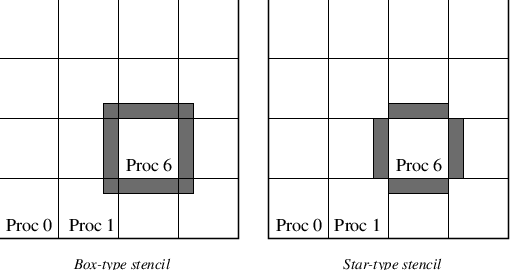
\psfig{file=ghost.eps,angle=0}}
\caption{Ghost Points for Two Stencil Types on the Seventh Processor}
\label{fig:ghosts}
\end{figure}

\subsection{Creating Distributed Arrays}

One creates a distributed array in two dimensions with the command 
\begin{verbatim}
   ierr = DACreate2d(MPI_Comm comm,DAPeriodicType wrap,DAStencilType st,int M,
                     int N,int m,int n,int dof,int s,int *lx,int *ly,DA *da);
\end{verbatim}
The \findex{DACreate2d} \sindex{array, distributed} arguments
\sindex{distributed array} {\tt M} and {\tt N} indicate the global
numbers of grid points in each direction, while {\tt m} and {\tt n}
denote the processor partition in each direction; {\tt m*n} must equal
the number of processors in the MPI communicator, {\tt comm}.  
Instead of specifying the processor layout, one may use
{\tt PETSC\_DECIDE} for {\tt m} and {\tt n} 
so that PETSc will determine the partition. The type of
periodicity of the array is specified by {\tt wrap}, which can be 
{\tt DA\_NONPERIODIC} \findex{DA_NONPERIODIC} (no periodicity), 
{\tt DA\_XYPERIODIC} \findex{DA_XYPERIODIC} (periodic in
both x- and y-directions), {\tt DA\_XPERIODIC} \findex{DA_XPERIODIC}, 
or {\tt DA\_YPERIODIC}.\findex{DA_YPERIODIC}  The argument {\tt dof} 
indicates the number of degrees of freedom at each array point,
and {\tt s} is the stencil width (i.e., the width of the ghost point region).
The optional arrays {\tt lx} and {\tt ly} may contain the number of nodes
along the x and y axis for each cell, i.e. the dimension of {\tt lx} is
{\tt m} and the dimension of {\tt ly} is {\tt n}; or {\tt PETSC\_NULL} 
may be passed in.

Two types of distributed arrays can be created, as specified by {\tt st}.
Star-type stencils that radiate outward only in the coordinate
directions are indicated by {\tt DA\_STENCIL\_STAR}
\findex{DA_STENCIL_STAR}, while box-type stencils are specified by
{\tt DA\_STENCIL\_BOX}. \findex{DA_STENCIL_BOX} For example, for the
two-dimensional case,
{\tt DA\_STENCIL\_STAR} with width 1 corresponds to the standard 5-point
stencil, while {\tt DA\_STENCIL\_BOX} with width 1 denotes the
standard 9-point stencil.  In both instances the ghost points are
identical, the only difference being that with star-type stencils
certain ghost points are ignored, potentially decreasing substantially
the number of messages sent.  Note that the {\tt DA\_STENCIL\_STAR}
stencils can save interprocessor communication in two and three
dimensions.

These {\tt DA} stencils have nothing directly to do with any finite
difference stencils one might chose to use for a discretization; they
only ensure that the correct values are in place for application of a
user-defined finite difference stencil (or any other
discretization technique).

The commands for creating distributed arrays in one and three
dimensions are analogous:
\findex{DACreate3d()} \findex{DACreate1d()} \findex{DACreate3d()}
\begin{verbatim}
   ierr = DACreate1d(MPI_Comm comm,DAPeriodicType wrap,int M,int w,int s,int *lc,DA *inra);
   ierr = DACreate3d(MPI_Comm comm,DAPeriodicType wrap,DAStencilType stencil_type,
                     int M,int N,int P,int m,int n,int p,int w,int s,int *lx,
                     int *ly,int *lz,DA *inra);
\end{verbatim}
{\tt DA\_ZPERIODIC}, \findex{DA_ZPERIODIC}
{\tt DA\_XZPERIODIC}, \findex{DA_XZPERIODIC}
{\tt DA\_YZPERIODIC}, and \findex{DA_YZPERIODIC}
{\tt DA\_XYZPERIODIC} \findex{DA_XYZPERIODIC}
are additional options in three dimensions for {\tt DAPeriodicType}.
The routines to create distributed arrays are collective, so that all
processors in the communicator {\tt comm} must call {\tt DACreateXXX()}.

\subsection{Local/Global Vectors and Scatters}

Each {\tt DA} object contains two vectors: a distributed global vector
and a local vector that includes the appropriate ghost points. These
vectors can be accessed \findex{DAGetLocalVector()}
with the routines \findex{DAGetDistributedVector}
\begin{verbatim}
   ierr = DAGetDistributedVector(DA da,Vec *g);
   ierr = DAGetLocalVector(DA da,Vec *l);
\end{verbatim}
These two vectors will generally serve as the building blocks for
local and global PDE solutions, etc.  Note that calling {\tt
DAGetDistributedVector()} or {\tt DAGetLocalVector()} does {\em not}
create a new vector object, but rather extracts the one existing
vector of its type from the distributed array.  Thus, if additional
vectors are needed in a code, they can be obtained by duplicating {\tt l}
or {\tt g} via {\tt VecDuplicate()} or {\tt VecDuplicateVecs()}.

At certain stages of many applications, there is a need to work 
on a local portion of the vector, including the ghost points. 
This may be done by scattering a global vector into its 
local parts by using the two-stage commands
\begin{verbatim}
   ierr = DAGlobalToLocalBegin(DA da,Vec g,InsertMode iora,Vec l);
   ierr = DAGlobalToLocalEnd(DA da,Vec g,InsertMode iora,Vec l);
\end{verbatim}
which allow the overlap of communication and computation.
\findex{DAGlobalToLocalEnd()}  \findex{DAGlobalToLocalBegin()}
Since the global and local vectors, given by {\tt g} and {\tt l}, respectively,
must be compatible with the distributed array, {\tt da}, they should be
generated by {\tt DAGetDistributedVector()} 
\findex{DAGetDistributedVector()} and {\tt DAGetLocalVector()}
\findex{DAGetLocalVector()}
(or be duplicates of such a vector obtained via {\tt VecDuplicate()}).
The {\tt InsertMode} can be either {\tt ADD\_VALUES} or {\tt INSERT\_VALUES}.

One can scatter the local patches into the distributed vector
with the command \findex{DALocalToGlobal()}
\begin{verbatim}
   ierr = DALocalToGlobal(DA da,Vec l,InsertMode mode,Vec g);
\end{verbatim}
Note that this function is not
subdivided into beginning and ending phases, since it is purely local.

A third type of distributed array scatter is from a local
vector (including ghost points that contain irrelevant values) to 
a local vector with correct ghost point values. 
This scatter may be done by \findex{DALocalToLocalBegin()}
commands \findex{DALocalToLocalEnd()}
\begin{verbatim}
   ierr = DALocalToLocalBegin(DA da,Vec l1,InsertMode iora,Vec l2);
   ierr = DALocalToLocalEnd(DA da,Vec l1,InsertMode iora,Vec l2);
\end{verbatim}
Since both local vectors, {\tt l1} and {\tt l2},
must be compatible with the distributed array, {\tt da}, they should be
generated by {\tt DAGetLocalVector()} \findex{DAGetLocalVector()}
(or be duplicates of such vectors obtained via {\tt VecDuplicate()}).
The {\tt InsertMode} can be either {\tt ADD\_VALUES} or {\tt INSERT\_VALUES}.

It is possible to directly access the vector scatter contexts 
used in the local-to-global ({\tt ltog}), global-to-local 
({\tt gtol}), and local-to-local ({\tt ltol})
scatters with the command \findex{DAGetScatter()}
\begin{verbatim}
   ierr = DAGetScatter(DA da,VecScatter *ltog,VecScatter *gtol,VecScatter *ltol);
\end{verbatim}
Most users should not need to use these contexts.

\subsection{Grid Information}

The global indices of the lower left corner of the local portion of the array 
as well as the local array size can be obtained with the commands
\findex{DAGetCorners()} \findex{DAGetGhostCorners()}
\begin{verbatim}
   ierr = DAGetCorners(DA da,int *x,int *y,int *z,int *m,int *n,int *p);
   ierr = DAGetGhostCorners(DA da,int *x,int *y,int *z,int *m,int *n,int *p);
\end{verbatim}
The first version excludes any ghost points, while the second version
includes them. Note that for interior subarrays the ghost corners can
easily be calculated from the true corners.  However, since the
calculation of ghost corners for boundary subarrays is not so
straightforward, both routines are provided.
The routine \findex{DAGetGhostCorners()} {\tt DAGetGhostCorners()}
deals with the fact that subarrays along boundaries of the problem
domain have ghost points only on their interior edges, but not on
their boundary edges.

When either type of stencil is used, {\tt DA\_STENCIL\_STAR} or 
{\tt DA\_STENCIL\_BOX}, the local vectors (with the ghost points) 
represent rectangular arrays, including the extra corner elements in 
the {\tt DA\_STENCIL\_STAR} case. This configuration provides simple 
access to the elements by employing two- (or three-) dimensional indexing. 
The only difference between the 
two cases is that when {\tt DA\_STENCIL\_STAR} is used, the extra 
corner components are {\em not} scattered between the processors and thus
contain undefined values that should {\em not} be used.

To assemble global stiffness matrices, one needs to be 
able to determine the global node number of each local node 
including the ghost nodes. The number may be determined by using the 
command \findex{DAGetGlobalIndices()}
\begin{verbatim}
   ierr = DAGetGlobalIndices(DA da,int *n,int **idx);
\end{verbatim}
The output argument {\tt n} contains the number of 
local nodes, including ghost nodes, while {\tt idx} contains
a list of the global indices that correspond to the local nodes.
Note that the Fortran interface differs slightly; see Section~\ref{sec:fortranarrays}
for details.

Since the global ordering that PETSc uses to manage its parallel vectors 
(and matrices) does not usually correspond to the ``natural'' ordering 
of a two- or three-dimensional array, the {\tt DA} structure provides 
an application ordering {\tt AO} (see Section \ref{sec:ao}) that maps 
between the natural ordering on a rectangular grid and the ordering PETSc
uses to parallize. This ordering context can be obtained with the command
\begin{verbatim}
   ierr = DAGetAO(DA da,AO *ao);
\end{verbatim}
\findex{DAGetAO}
In Figure \ref{fig:daao} we indicate the orderings for a two-dimensional distributed 
array, divided among four processors.

\begin{figure}[tb]
\centerline{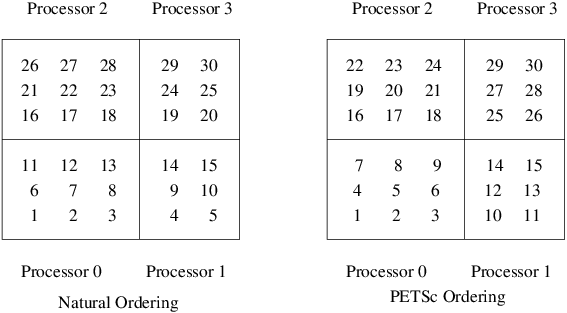
\psfig{file=../pictures/danumbering.eps,angle=270,width=4.7in}}
\caption{Natural Ordering and PETSc Ordering for a 2D Distributed Array (Four Processors)}
\label{fig:daao}
\end{figure}

The example
{\tt \$(PETSC\_DIR)/src/snes/examples/tutorials/ex5.c},
illustrates the use of a distributed array in the solution of
a nonlinear problem.  The analogous Fortran program is
\break {\tt \$(PETSC\_DIR)/src/snes/examples/tutorials/ex5f.F};
See Chapter \ref{chapter:snes} for a discussion of the nonlinear
solvers.

%\begin{figure}[H]
%{\small
%\fileinclude{../../../src/snes/examples/tutorials/ex5.c}
%}
%\caption{Use of Distributed Arrays}
%\label{fig:daexample}
%\end{figure}

% -------------------------------------------------------------------------------------- 
\section{Software for Managing Unstructured Grids}
\label{sec:unstruct}

% -------------------------------------------------------------------------------------- 
\subsection{Index Sets} \sindex{index sets}
\label{sec:indexset}

To facilitate general vector scatters and gathers, PETSc employs the 
concept of an index set.  An index set, which is a generalization of a 
set of integer indices, is used to define scatters, gathers, and similar 
operations on vectors and matrices. 

The following command creates a sequential index set based on a list 
of integers: \findex{ISCreateGeneral()}
\begin{verbatim}
   ierr = ISCreateGeneral(MPI_Comm comm,int n,int *indices, IS *is);
\end{verbatim}
This routine essentially copies the {\tt n} indices passed 
to it by the integer array {\tt indices}.  
Thus, the user should be sure to free the integer array {\tt indices} 
when it is no longer needed, perhaps directly after the call to 
{\tt ISCreateGeneral()}. The communicator, {\tt comm}, should consist of only
one processor (often {\tt comm=MPI\_COMM\_SELF}).

Another standard index set is defined by a starting point ({\tt first}) and a
stride ({\tt step}), \sindex{stride} and can be created with the command
\begin{verbatim}
   ierr = ISCreateStride(MPI_Comm comm,int n,int first,int step,IS *is);
\end{verbatim}
Again, the {\tt comm} argument should always consist of
a communicator with one processor, often {\tt MPI\_COMM\_SELF}.

There is no parallel general index set. Instead, one should create a sequential
index set on each processor that needs one.
Index sets can be destroyed with the command \findex{ISDestroy()}
\begin{verbatim}
   ierr = ISDestroy(IS is); 
\end{verbatim}

On rare occasions the user may have to access information directly 
from an index set. \findex{ISGetSize()} 
Several commands \findex{ISStrideGetInfo()} \findex{ISGetIndices()}
assist in this process:
\begin{verbatim}
   ierr = ISGetSize(IS is,int *size);
   ierr = ISStrideGetInfo(IS is,int *first,int *stride);
   ierr = ISGetIndices(IS is,int **indices);
\end{verbatim}
The function {\tt ISGetIndices()} returns a pointer to a list of the 
indices in the index set. 
For certain index sets, this may be a 
temporary array of indices created specifically for a given routine. 
Thus, once the user finishes using the array of indices, 
the routine \findex{ISRestoreIndices()}
\begin{verbatim}
   ierr = ISRestoreIndices(IS is, int **indices); 
\end{verbatim}
should be called to ensure that the system can free the space it 
may have used to generate the list of indices.

A blocked version of the index sets can be created with the command
\findex{ISCreateBlock}
\begin{verbatim}
   ierr = ISCreateBlock(MPI_Comm comm,int bs,int n,int *indices, IS *is);
\end{verbatim}
This version is used for defining operations in which each element of the index
set refers to a block of {\tt bs} vector entries.  Related routines analogous
to those described above exist as well, including
{\tt ISBlockGetIndices()}, {\tt ISBlockGetSize()}, {\tt ISBlockGetBlockSize()},
and {\tt ISBlock()}. See the man pages for details.
\findex{ISBlockGetIndices()} \findex{ISBlockGetSize()} \findex{ISBlockGetBlockSize()}
\findex{ISBlock()}

One may reasonably ask why the scatter routines are based on 
using index sets while the vector assembly routines simply use 
arrays of integers. The reason for using index sets is to allow certain 
implementations to deal with strides and dense blocks of elements 
efficiently. In vector assembly, we are assuming that in the majority of 
cases the gain from using index sets is more than lost by requiring 
the users to build index sets for each insertion. 

% -------------------------------------------------------------------------------------- 
\subsection{Scatters and Gathers} \sindex{scatter} \sindex{gather}
\label{sec:scatter}

PETSc vectors have full support for general scatters and 
gathers. One can select any subset of the components of a vector to
insert or add to any subset of the components of another vector.
We refer to these operations as generalized scatters, though they are 
actually a combination of scatters and gathers. 

\findex{VecScatterCreate()} \findex{VecScatterBegin()}
\findex{VecScatterEnd()} \findex{VecScatterDestroy()}
\findex{INSERT_VALUES} \findex{SCATTER_FORWARD}
To copy selected components from one vector 
to another, one uses the following set of commands:
\begin{verbatim}
   ierr = VecScatterCreate(Vec x,IS ix,Vec y,IS iy,VecScatter *ctx);
   ierr = VecScatterBegin(Vec x,Vec y,INSERT_VALUES,SCATTER_FORWARD,VecScatter ctx);
   ierr = VecScatterEnd(Vec x,Vec y,INSERT_VALUES,SCATTER_FORWARD,VecScatter ctx);
   ierr = VecScatterDestroy(VecScatter ctx);
\end{verbatim} 
Here {\tt ix} denotes the index set of the first vector, while {\tt
iy} indicates the index set of the destination vector.  The vectors
can be parallel or sequential. The only requirements are that the
number of entries in the index set of the first vector, {\tt ix},
equal the number in the destination index set, {\tt iy}, and that the
vectors be long enough to contain all the indices referred to in the
index sets.  The argument {\tt INSERT\_VALUES} specifies that the
vector elements will be inserted into the specified locations of the
destination vector, overwriting any existing values.  To add the
components, rather than insert them, the user should select the option
{\tt ADD\_VALUES} \findex{ADD_VALUES} instead of {\tt INSERT\_VALUES}.

To perform a conventional gather operation, the user simply makes
 the destination index set, 
{\tt iy}, be a stride index set with a stride of one.  Similarly, a 
conventional scatter can be done with an initial (sending) index set 
consisting of a stride.  For parallel vectors, all processors that own 
the vector {\em must} call the scatter routines. When scattering from a 
parallel vector to sequential vectors, each processor has its own sequential 
vector that receives values from locations as indicated in its own 
index set. Similarly, in scattering
from sequential vectors to a parallel vector, each processor has its
own sequential vector that makes contributions to the parallel vector.

{\em Caution}: When {\tt INSERT\_VALUES} is used, if two different
processors contribute different values to the same component in a
parallel vector, either value may end up being inserted. When {\tt
ADD\_VALUES} is used, the correct sum is added to the correct
location.

In some cases one may wish to ``undo'' a scatter, that is perform the 
scatter backwards switching the roles of the sender and receiver. This is 
done by using 
\begin{verbatim}
   ierr = VecScatterBegin(Vec y,Vec x,INSERT_VALUES,SCATTER_REVERSE,VecScatter ctx);
   ierr = VecScatterEnd(Vec y,Vec x,INSERT_VALUES,SCATTER_REVERSE,VecScatter ctx);
\end{verbatim} 
\findex{SCATTER_REVERSE} Note that you must swap the roles of the first 
two arguments to these routines, whenever you use the {\tt SCATTER\_REVERSE}
option.

\sindex{vector values, getting} \findex{VecGetValues()}
There is no PETSc routine that is the opposite of {\tt VecSetValues()}
\findex{VecSetValues()}, that is, {\tt VecGetValues()}. \findex{VecGetValues()}
Instead, the user should create a new vector where
the components are to be stored and perform the appropriate vector 
scatter. For example, if one desires to obtain the values of the 
100th and 200th entries of a parallel vector, {\tt p}, one could use 
a code such as that within Figure~\ref{fig:vecscatter}.
In this example, the values of the 100th and 200th components are
placed in the array 
{\tt values}. In this example each processor now has the 100th and 
200th component, but obviously each processor could gather any 
elements it needed, or none by creating an index set with no entries.

\begin{figure}[tb]
\begin{verbatim}
   Vec        p, x;         /* initial vector, destination vector */
   VecScatter scatter;      /* scatter context */
   IS         from, to;     /* index sets that define the scatter */
   Scalar     *values;
   int        idx_from[] = {100,200}, idx_to[] = {0,1};

   VecCreateSeq(PETSC_COMM_SELF,2,&x);
   ISCreateGeneral(PETSC_COMM_SELF,2,idx_from,&from);
   ISCreateGeneral(PETSC_COMM_SELF,2,idx_to,&to);
   VecScatterCreate(p,from,x,to,&scatter);
   VecScatterBegin(p,x,INSERT_VALUES,SCATTER_FORWARD,scatter);
   VecScatterEnd(p,x,INSERT_VALUES,SCATTER_FORWARD,scatter);
   VecGetArray(x,&values);
   ISDestroy(from);
   ISDestroy(to); 
   VecScatterDestroy(scatter);
\end{verbatim}
\caption{Example Code for Vector Scatters}
\label{fig:vecscatter}
\end{figure}

The scatter comprises two stages, in order to allow overlap of 
communication and computation. The introduction of the 
{\tt VecScatter} context allows the communication patterns for the scatter
to be computed once and then reused repeatedly. Generally, even 
setting up the communication for a scatter requires communication; 
hence, it is best to reuse such information when possible.

% -------------------------------------------------------------------------------
\subsection{Scattering Ghost Values}


The scatters provide a very general method for managing the communication of 
required ghost values for unstructured grid computations. One scatters
the global vector into a local ``ghosted'' work vector and performs the computation
on the local work vectors and then scatters back into the global solution 
vector. In the simplest case this may be written as
\begin{verbatim}
   Function: (Input Vec globalin, Output Vec globalout)

   ierr = VecScatterBegin(Vec globalin,Vec localin,InsertMode INSERT_VALUES,ScatterMode
                          SCATTER_FORWARD,VecScatter scatter);
   ierr = VecScatterEnd(Vec globalin,Vec localin,InsertMode INSERT_VALUES,ScatterMode
                          SCATTER_FORWARD,VecScatter scatter);
   /*
        For example,  do local calculations from localin to localout and call
   */
   ierr = VecScatterBegin(Vec localout,Vec globalout,InsertMode ADD_VALUES,ScatterMode
                          SCATTER_REVERSE,VecScatter scatter);
   ierr = VecScatterEnd(Vec localout,Vec globalout,InsertMode ADD_VALUES,ScatterMode
                          SCATTER_REVERSE,VecScatter scatter);
\end{verbatim}

% -------------------------------------------------------------------------------
\subsection{Vectors with Locations for Ghost Values}

We recommend that application developers skip this section on a first reading.
It contains information about more advanced use of PETSc vectors to improve 
efficiency slightly. Once your application code is fully debugged and optimized
you can try to use these techniques to slightly decrease memory use and improve 
computation speed slightly.

There are two minor (IMHO) drawbacks to this approach:
\begin{itemize}
\item the extra memory requirement for the local work vector, {\tt localin} that
      duplicates the memory in {\tt globalin},
\item the extra time required to copy the local values from {\tt localin} to 
      {\tt globalin}.
\end{itemize}

An alternative approach is to allocate global vectors with space preallocated for 
the ghost values; this may be done with either 
\begin{verbatim}
   ierr = VecCreateGhost(MPI_Comm comm,int n,int N,int nghost,int *ghosts,Vec *vv)
\end{verbatim}
or
\begin{verbatim}
   ierr = VecCreateGhostWithArray(MPI_Comm comm,int n,int N,int nghost,int *ghosts,
                                  Scalar *array,Vec *vv)
\end{verbatim}
Here \findex{VecCreateGhost()} \findex{VecCreateGhostWithArray()} {\tt n} is the 
number of local vector entries, {\tt N} is the number of \sindex{vectors, with ghost values}
global entries (or {\tt PETSC\_NULL}) and {\tt nghost} is the number of 
ghost entries. The array {\tt ghosts} is of size {\tt nghost} and contains the 
global vector location for each local ghost location. Using {\tt VecDuplicate()}
or {\tt VecDuplicateVecs()} on a ghosted vector will generate additional ghosted vectors.

In many ways a ghosted vector behaves just like any other {\tt MPI} vector created 
by {\tt VecCreateMPI()}, the difference is that the ghosted vector has an additional 
``local'' representation that allows one to access the ghost locations. This is done
through the call to \findex{VecGhostGetLocalRepresentation()} 
\begin{verbatim}
  ierr = VecGhostGetLocalRepresentation(Vec g,Vec *l);
\end{verbatim}
The vector {\tt l} is a \findex{VecGhostRestoreLocalRepresentation()}
sequential representation of the parallel vector {\tt g} 
that shares the same array space (and hence numerical values); but allows one to 
access the ``ghost'' values past ``the end of the'' array. Note that one access the 
entries in {\tt l} using the local numbering of elements and ghosts, while they 
access in {\tt g} using the global numbering.

A common usage of a ghosted
vector could be given by \findex{VecGhostUpdateBegin()} \findex{VecGhostUpdateEnd()}
\begin{verbatim}
   ierr = VecGhostUpdateBegin(Vec globalin,InsertMode INSERT_VALUES,ScatterMode
                          SCATTER_FORWARD);
   ierr = VecGhostUpdateEnd(Vec globalin,InsertMode INSERT_VALUES,ScatterMode
                          SCATTER_FORWARD);
   ierr = VecGhostGetLocalRepresentation(Vec globalin,Vec *localin);
   ierr = VecGhostGetLocalRepresentation(Vec globalout,Vec *localout);
   /*
      Do local calculations from localin to localout 
   */
   ierr = VecGhostRestoreLocalRepresentation(Vec globalin,Vec *localin);
   ierr = VecGhostRestoreLocalRepresentation(Vec globalout,Vec *localout);
   ierr = VecGhostUpdateBegin(Vec globalout,InsertMode ADD_VALUES,ScatterMode
                          SCATTER_REVERSE);
   ierr = VecGhostUpdateEnd(Vec globalout,InsertMode ADD_VALUES,ScatterMode
                          SCATTER_REVERSE);
\end{verbatim}
      
The routines {\tt VecGhostUpdateBegin/End()} are equivalent to {\tt VecScatterBegin/End()}
above except that since they are scattering into the ghost locations they do not need
to copy the local vector values (they are already there). In addition the user does not
have to allocate the local work vector, since the ghosted vector already has allocated 
slots to contain the ghost values.

The use of the arguments {\tt INSERT\_VALUES} and {\tt SCATTER\_FORWARD } causes the 
ghost values to be correctly updated from the appropriate processor. The arguments
{\tt ADD\_VALUES} and {\tt SCATTER\_REVERSE } update the ``local'' portions of the vector 
from all the other processors ghost values; this would be appropriate, for example, for
finite element assembly of the load vector. 



%-------------------------------------------------------------
%-------------------------------------------------------------
\chapter{Matrices}
\label{chapter:matrices}
\sindex{matrices}

PETSc 2.0 provides a variety of matrix implementations because no
single matrix format is appropriate for all problems.  Currently we
support dense storage and compressed sparse row storage (both
sequential and parallel versions), as well as several specialized
formats.  Additional formats can be added easily.

This chapter describes the basics of using PETSc matrices in general
(regardless of the particular format chosen) and discusses tips
for efficient use of the several simple uniprocessor and parallel
matrix types.  Details regarding the ever-expanding suite of
PETSc matrices are given in Section~\ref{sec:matclasses}.
The use of PETSc matrices involves the following actions: create a
particular type of matrix, insert values into it, process the matrix,
use the matrix for various computations, and finally destroy the
matrix.  The application code does not need to know or care about the
particular storage formats of the matrices.

\section{Creating and Assembling Matrices}
\label{sec:matcreate}

The simplest routine for forming a PETSc matrix, {\tt A}, is \findex{MatCreate()}
\begin{verbatim}
   ierr = MatCreate(MPI_Comm comm,int M,int N,Mat *A)
\end{verbatim}
This routine generates a sequential matrix when running on one
processor and a parallel matrix for two or more processors; the
particular matrix format is set by the user via options database
commands.  The user specifies only the global matrix dimensions, given
by {\tt M} and {\tt N}, while PETSc determines the appropriate local
dimensions and completely controls memory allocation.  This routine
facilitates switching among various matrix types, for example, to
determine the format that is most efficient for a certain
application.  By default, {\tt MatCreate()} employs the sparse AIJ
format, which is discussed in detail Section~\ref{sec:matsparse}.  See
the man page for further information about available matrix formats.

To insert or add entries to a matrix, one can call a variant of {\tt
MatSetValues}, either \findex{MatSetValues()}
\begin{verbatim}
   ierr = MatSetValues(Mat A,int m,int *im,int n,int *in,Scalar *values,INSERT_VALUES);
\end{verbatim}
or 
\begin{verbatim}
   ierr = MatSetValues(Mat A,int m,int *im,int n,int *in,Scalar *values,ADD_VALUES);
\end{verbatim}
This routine inserts or adds a logically dense subblock of dimension
{\tt m*n} into the 
matrix. The integer indices {\tt im} and {\tt in}, respectively, indicate the 
global row and column numbers to be inserted.  {\tt MatSetValues()} uses the 
standard C convention, where the row and column matrix indices begin with 
zero {\em regardless of the storage format employed}.   The array 
{\tt values} is logically two-dimensional, containing the values that are 
to be inserted.   
By default the values are given in row major order, which is the opposite 
of the Fortran convention. To allow the insertion of values in column 
major order, one can call the command \findex{MatSetOption()}
\begin{verbatim}
   ierr = MatSetOption(Mat A,MAT_COLUMN_ORIENTED);
\end{verbatim}
{\bf Warning}: Several of the sparse implementations do {\em not} currently support
the column-oriented option!

This notation should not be a mystery to anyone. For example, 
to insert one matrix into another when using Matlab, one uses the command 
{\tt A(im,in) = B;} where {\tt im} and {\tt in} contain the indices for the
rows and columns. This action is identical to the calls above to 
{\tt MatSetValues()}.

When using the block compressed sparse row matrix format ({\tt MATSEQBAIJ} or
{\tt MATMPIBAIJ}), one can insert elements more efficiently using the block
variant, {\tt MatSetValuesBlocked()}. \findex{MatSetValuesBlocked()}

The function {\tt MatSetOption()} accepts several other inputs; see
the man page for details. We
discuss two of these options, which are related to the efficiency of the
assembly process.  To indicate to PETSc that the row ({\tt im}) or
column ({\tt in}) indices set with {\tt MatSetValues()} are sorted,
one uses the command \findex{MAT_ROWS_SORTED} \findex{MAT_COLUMNS_SORTED}
\begin{verbatim}
   ierr = MatSetOption(Mat A,MAT_ROWS_SORTED);
\end{verbatim}
or 
\begin{verbatim}
   ierr = MatSetOption(Mat A,MAT_COLUMNS_SORTED);
\end{verbatim}

After the matrix elements have been inserted or added into the matrix, 
it must be processed before it can be used. The routines for matrix
processing are \findex{MatAssemblyBegin()} \findex{MatAssemblyEnd()}
\begin{verbatim}
   ierr = MatAssemblyBegin(Mat A,MAT_FINAL_ASSEMBLY);
   ierr = MatAssemblyEnd(Mat A,MAT_FINAL_ASSEMBLY);
\end{verbatim}
By placing other code between these two calls, the user can perform
computations while messages are in transition.
Calls to {\tt MatSetValues()} with the {\tt INSERT\_VALUES} and {\tt
ADD\_VALUES} options {\em cannot} be mixed without intervening calls to
the assembly routines.  For such intermediate assembly calls the
second routine argument  typically should be {\tt MAT\_FLUSH\_ASSEMBLY},
\findex{MAT_FLUSH_ASSEMBLY} which omits some of the work of the full 
assembly process.  {\tt MAT\_FINAL\_ASSEMBLY} \findex{MAT_FINAL_ASSEMBLY} is
required only in the last matrix assembly before a matrix is used.

Even though one may insert values into PETSc matrices without regard
to which processor eventually stores them, for efficiency
reasons we usually recommend generating most entries on the
processor where they are destined to be stored.  To help the
application programmer with this task for matrices that are
distributed across the processors by ranges, the routine
\findex{MatGetOwnershipRange()}
\begin{verbatim}
   ierr = MatGetOwnershipRange(Mat A,int *first_row,int *last_row);
\end{verbatim}
informs the user that all rows from {\tt first\_row} to 
{\tt last\_row-1} will be stored on the local processor.

In the sparse matrix implementations, once the assembly routines have been 
called, the matrices are compressed and can be used for matrix-vector
multiplication, etc.
Inserting new values into the matrix at this point will be expensive, 
since it requires copies and possible memory allocation. Thus, whenever 
possible one should completely set the values in the matrices before 
calling the final assembly routines. 

If one wishes to repeatedly assemble matrices that retain the same
nonzero pattern (such as within a nonlinear or time-dependent
problem), the option
\begin{verbatim}
   ierr = MatSetOption(Mat mat,MAT_NO_NEW_NONZERO_LOCATIONS);
\end{verbatim}
should be specified after the first matrix has been fully assembled.
This option ensures that certain data structures and communication
information will be reused (instead of regenerated) during successive
steps, thereby increasing efficiency.  
See {\tt \$(PETSC\_DIR)/src/sles/examples/tutorials/ex5.c} for a simple example of
solving two linear systems that use the same matrix data structure.

\subsection{Sparse Matrices}
\label{sec:matsparse}

\sindex{AIJ matrix format} 
\sindex{CSR, compressed sparse row format}
The default matrix representation within PETSc is the general sparse 
AIJ format (also called the Yale sparse matrix format or compressed
sparse row format, CSR).  This section discusses tips for {\em efficiently}
using this matrix format for large-scale applications. Additional
formats (such as block compressed row and block diagonal storage,
which are generally much more efficient for problems with multiple
degrees of freedom per node) are further discussed in
Section~\ref{sec:matclasses}.  Beginning users need not concern
themselves initially with such details and may wish to proceed
directly to Section~\ref{sec:matoptions}.  However, when an
application code progresses to the point of tuning for efficiency
and/or generating timing results, it is {\em crucial} to read this
information.

\subsubsection{Sequential AIJ Sparse Matrices}

In the PETSc AIJ matrix formats, we store the nonzero elements
by rows, along with an array of corresponding column numbers and
an array of pointers to the beginning of each row.  Note that the
diagonal matrix entries are stored with the rest of the nonzeros (not
separately). 

To create a sequential AIJ sparse matrix, {\tt A}, 
\findex{MatCreateSeqAIJ()} with {\tt m} rows and {\tt n} columns,
one uses the command
\begin{verbatim}
   ierr = MatCreateSeqAIJ(PETSC_COMM_SELF,int m,int n,int nz,int *nzz,Mat *A);
\end{verbatim}
where {\tt nz} or {\tt nnz} can be used to preallocate matrix memory,
as discussed below. The user can set {\tt nz=0} and {\tt
nzz=PETSC\_NULL} for PETSc to control all matrix memory allocation.

The sequential and parallel AIJ matrix storage formats by default
employ {\em i-nodes} (identical nodes) when possible.  We search for
consecutive rows with the same nonzero structure, thereby reusing
matrix information for increased efficiency.  Related options database
keys are {\tt -mat\_aij\_no\_inode} (do not use inodes) and {\tt
-mat\_aij\_inode\_limit <limit>} (set inode limit (max limit=5)).

By default the internal data representation for the AIJ formats employs
zero-based indexing.  For compatibility with standard Fortran storage,
thus enabling use of external Fortran software packages such as
SPARSKIT, \sindex{SPARSKIT} the option {\tt -mat\_aij\_oneindex}
\findex{-mat_aij_oneindex} enables one-based indexing, where the stored
row and column indices begin at one, not zero.  All user calls to
PETSc routines, regardless of this option, use zero-based indexing.

\subsubsection{Preallocation of Memory for Sequential AIJ Sparse Matrices}

The dynamic process of allocating new memory and copying from the old
storage to the new is {\em intrinsically very expensive}.  Thus, to
obtain good performance when assembling an AIJ matrix, it is crucial
to preallocate the memory needed for the sparse matrix.  The user has
two choices for preallocating matrix memory via {\tt
MatCreateSeqAIJ()}. 

One can use the scalar {\tt nz} to specify the expected
number of nonzeros for each row.  This is generally fine if the number
of nonzeros per row is roughly the same throughout the matrix (or as a
quick and easy first step for preallocation).  If one underestimates
the actual number of nonzeros in a given row, then during the assembly
process PETSc will automatically allocate additional needed space.
However, this extra memory allocation can slow the computation,

Thus, if different rows have very different numbers of nonzeros, one
should attempt to indicate (nearly) the exact number of elements
intended for the various rows with the optional array, {\tt nzz} of
length {\tt m}, where {\tt m} is the number of rows, for example
\begin{verbatim}
   int nnz[m];
   nnz[0] = <nonzeros in row 0>
   nnz[1] = <nonzeros in row 1>
   ....
   nnz[m-1] = <nonzeros in row m-1>
\end{verbatim}
In this case, the assembly process will require no additional memory
allocations if the {\tt nnz} estimates are correct. If, however,
the {\tt nnz} estimates are incorrect, PETSc will automatically
obtain the additional needed space, at a slight loss of efficiency.

Using the array {\tt nnz} to preallocate memory is especially
important for efficient matrix assembly if the number of nonzeros
varies considerably among the rows.  One can generally set {\tt nnz}
either by knowing in advance the problem structure (e.g., the stencil
for finite difference problems on a structured grid) or by
precomputing the information by using a segment of code similar to
that for the regular matrix assembly.  The overhead of determining the
{\tt nnz} array will be quite small compared with the overhead of the
inherently expensive mallocs and moves of data that are needed for
dynamic allocation during matrix assembly.

Thus, when assembling a sparse matrix with very different
numbers of nonzeros in various rows, one could proceed 
as follows for finite difference methods:
\begin{tabbing}
12\=12\= \kill
    \> - Allocate integer array {\tt nnz}.\\
    \> - Loop over grid, counting the expected number of nonzeros for the row(s)\\
    \>\>  associated with the various grid points.\\
    \> - Create the sparse matrix via {\tt MatCreateSeqAIJ()} or alternative.\\
    \> - Loop over the grid, generating matrix entries and inserting 
      in matrix via {\tt MatSetValues()}.\\
  \end{tabbing}
\vspace{-0.2in}
For (vertex-based) finite element type calculations, an analogous procedure is as follows:
  \begin{tabbing}
12\=12\= \kill
    \> - Allocate integer array {\tt nnz}.\\
    \>- Loop over vertices, computing the number of neighbor vertices, which determines the\\
    \>\> number of nonzeros for the corresponding matrix row(s).\\
    \> - Create the sparse matrix via {\tt MatCreateSeqAIJ()} or alternative.\\
    \> - Loop over elements, generating matrix entries and inserting
      in matrix via {\tt MatSetValues()}.\\
  \end{tabbing}

The {\tt -log\_info} \findex{-log_info} option causes the routines
{\tt MatAssemblyBegin()} and {\tt MatAssemblyEnd()} to print
information about the success of the preallocation.  Consider the
following example for the {\tt MATSEQAIJ} matrix format:
\begin{verbatim}
   MatAssemblyEnd_SeqAIJ:Matrix size 100 X 100; storage space: 2000 unneeded, 1000 used
   MatAssemblyEnd_SeqAIJ:Number of mallocs during MatSetValues is 0
\end{verbatim}
The first line indicates that the user preallocated 3000 spaces but only
1000 were used. The second line indicates that the user preallocated
enough space so that PETSc did not have to internally allocate additional
space (an expensive operation).  In the next example the user did not
preallocate sufficient space, as indicated by the fact that the number
of mallocs is very large (bad for efficiency):
\begin{verbatim}
   MatAssemblyEnd_SeqAIJ:Matrix size 1000 X 1000; storage space: 47 unneeded, 100000 used
   MatAssemblyEnd_SeqAIJ:Number of mallocs during MatSetValues is 40000
\end{verbatim}
 
Although at first glance such procedures for determining the matrix
structure in advance may seem unusual, they are actually very
efficient because they alleviate the need for dynamic
construction of the matrix data structure, which can be very
expensive.


\subsubsection{Parallel AIJ Sparse Matrices}

Parallel sparse matrices with the AIJ 
format can be created with the command \findex{MatCreateMPIAIJ()}
\begin{verbatim}
   ierr = MatCreateMPIAIJ(MPI_Comm comm,int m,int n,int M,int N,int d_nz,
                          int *d_nnz, int o_nz,int *o_nnz,Mat *A);
\end{verbatim}
{\tt A} is the newly created matrix, while the arguments {\tt m}, {\tt n}, 
{\tt M}, and {\tt N}, indicate the number of local rows and columns and
the number of global rows and columns, respectively. Either the local or
global parameters can be replaced with {\tt PETSC\_DECIDE}, so that 
PETSc will determine \findex{PETSC_DECIDE} them.
The matrix is stored with a fixed number of rows on 
each processor, given by {\tt m}, or determined by PETSc if {\tt m} is
{\tt PETSC\_DECIDE}.

If one does not use {\tt PETSC\_DECIDE} for
{\tt m} and {\tt n} then he must ensure that they are chosen to be
compatible with the vectors. To do this, one first considers the product 
$y = A x$. The {\tt m} that one uses in {\tt MatCreateMPIAIJ()}
must match the local size used in the {\tt VecCreateMPI()} for {\tt y}.
The {\tt n} used must match that used as the local size in 
{\tt VecCreateMPI()} for {\tt x}. 

The user must set {\tt d\_nz=0}, {\tt o\_nz=0}, {\tt d\_nnz=PETSC\_NULL}, and 
{\tt o\_nnz=PETSC\_NULL} for PETSc to control dynamic allocation of matrix
memory space.  Analogous to {\tt nz} and {\tt nnz} for the routine 
{\tt MatCreateSeqAIJ()}, these arguments optionally specify 
nonzero information for the diagonal ({\tt d\_nz} and {\tt d\_nnz}) and 
off-diagonal ({\tt o\_nz} and {\tt o\_nnz}) parts of the matrix. 
For a square global matrix, we define each processor's diagonal portion 
to be its local rows and the corresponding columns (a square submatrix);  
each processor's off-diagonal portion encompasses the remainder of the
local matrix (a rectangular submatrix).  
The rank in the MPI communicator determines the absolute ordering of the
blocks.  That is, the process with rank 0 in the communicator given to {\tt
  MatCreateMPIAIJ} contains the top rows of the matrix; the i$^{th}$ process
in that communicator contains the i$^{th}$ block of the matrix.

\subsubsection{Preallocation of Memory for Parallel AIJ Sparse Matrices}

As discussed above, preallocation of memory is critical for achieving good
performance during matrix assembly, as this reduces the number of
allocations and copies required.  We present an example for
three processors to indicate how this may be done for the {\tt MATMPIAIJ}
matrix format.  Consider the 8 by
8 matrix, which is partitioned by default with three rows on the first
processor, three on the second and two on the third.  {\small
\[
\left( \begin{array}{cccccccccc} 
1  & 2  & 0  & | & 0  & 3  & 0  & |  & 0  & 4  \\
0  & 5  & 6  & | & 7  & 0  & 0  & |  & 8  & 0 \\
9  & 0  & 10 & | & 11 & 0  & 0  & |  & 12 & 0  \\
\hline \\
13 & 0  & 14 & | & 15 & 16 & 17 & |  & 0  & 0  \\
0  & 18 & 0  & | & 19 & 20 & 21 & |  & 0  & 0 \\
0  & 0  & 0  & | & 22 & 23 & 0  & |  & 24 & 0 \\
\hline \\
25 & 26 & 27 & | & 0  & 0  & 28 & |  & 29 & 0 \\
30 & 0  & 0  & | & 31 & 32 & 33 & |  & 0  &34 
\end{array} \right)
\]
}

The ``diagonal'' submatrix, {\tt d}, on the first processor is given by 
{\small
\[
\left( \begin{array}{ccc} 
1  & 2  & 0  \\
0  & 5  & 6  \\
9  & 0  & 10 
\end{array} \right),
\]
}
while the ``off-diagonal'' submatrix, {\tt o}, matrix is given by 
{\small
\[
\left( \begin{array}{ccccc} 
 0  & 3  & 0   & 0  & 4  \\
 7  & 0  & 0   & 8  & 0  \\
 11 & 0  & 0   & 12 & 0  \\
\end{array} \right).
\]
}
For the first processor one could set {\tt d\_nz} to 2 (since each
row has 2 nonzeros) or, alternatively, set {\tt d\_nzz} to \{2,2,2\}.
The {\tt o\_nz} could be set to 2 since each row of the {\tt o} matrix
has 2 nonzeros, or {\tt o\_nzz} could be set to \{2,2,2\}.

For the second processor the {\tt d} submatrix is given by 
{\small
\[
\left( \begin{array}{cccccccccc} 
 15 & 16 & 17 \\
 19 & 20 & 21 \\
 22 & 23 & 0  
\end{array} \right) .
\]
}
Thus, one could set {\tt d\_nz} to 3, since the maximum number of
nonzeros in each row is 3, or alternatively one could set {\tt d\_nzz} to
\{3,3,2\}, thereby indicating that the first two rows will have 3
nonzeros while the third has 2. The corresponding {\tt o} submatrix for the
second processor is
{\small
\[
\left( \begin{array}{cccccccccc} 
13 & 0  & 14 &  0  & 0  \\
0  & 18 & 0  &  0  & 0 \\
0  & 0  & 0  &  24 & 0 \\
\end{array} \right)
\]
}
so that one could set {\tt o\_nz} to 2 or {\tt o\_nzz} to \{2,1,1\}.

Note that the user never directly works with the {\tt d} and {\tt o}
submatrices, except when preallocating storage space as indicated above.
Also, the user need not preallocate exactly the correct amount of
space; as long as a sufficiently close estimate is given, the high
efficiency for matrix assembly will remain.  

As described above, the option {\tt -log\_info} \findex{-log_info}
will print information about the success of preallocation during
matrix assembly.  For the {\tt MATMPIAIJ} format, PETSc will also list
the number of elements owned by on each processor that were generated
on a different processor.  For example, the statements
\begin{verbatim}
   [0]MatAssemblyBegin_MPIAIJ:Number of off processor values 10
   [1]MatAssemblyBegin_MPIAIJ:Number of off processor values 7
   [2]MatAssemblyBegin_MPIAIJ:Number of off processor values 5
\end{verbatim}
indicate that very few values have been generated on different processors.
On the other hand, the statements
\begin{verbatim}
   [0]MatAssemblyBegin_MPIAIJ:Number of off processor values 100000
   [1]MatAssemblyBegin_MPIAIJ:Number of off processor values 77777
\end{verbatim}
indicate that many values have been generated on the ``wrong'' processors.
This situation can be very inefficient, since the transfer of values
to the ``correct'' processor is generally expensive.  By using the command
{\tt MatGetOwnershipRange()} in application codes, the user should be able
to generate most entries on the owning processor.

{\em Note}: It is fine to generate some entries on the ``wrong'' processor. Often
this can lead to cleaner, simpler, less buggy codes.  One should never
make code overly complicated in order to generate all values locally. Rather,
one should organize the code in such a way that {\em most} values are generated locally.

\subsection{Dense Matrices}
\label{sec:matdense}

PETSc provides both sequential and parallel dense matrix formats,
where each processor stores its entries in a column-major array in the
usual Fortran style.  To create a sequential, dense PETSc matrix,
{\tt A} of dimensions {\tt m} by {\tt n}, the user should
call \findex{MatCreateSeqDense()}
\begin{verbatim}
   ierr = MatCreateSeqDense(PETSC_COMM_SELF,int m,int n,Scalar *data,Mat *A);
\end{verbatim}
The variable {\tt data} enables the user to optionally provide the
location of the data for matrix storage (intended for Fortran users who
wish to allocate their own storage space).  Most users should merely
set {\tt data} to {\tt PETSC\_NULL} for PETSc to control matrix memory allocation.
To create a parallel, dense matrix, {\tt A}, the user should call
\begin{verbatim}
   ierr = MatCreateMPIDense(MPI_Comm comm,int m,int n,int M,int N,Scalar *data,Mat *A)
\end{verbatim}
The arguments {\tt m}, {\tt n}, 
{\tt M}, and {\tt N}, indicate the number of local rows and columns and
the number of global rows and columns, respectively. Either the local or
global parameters can be replaced with {\tt PETSC\_DECIDE}, so that 
PETSc will determine \findex{PETSC_DECIDE} them.
The matrix is stored with a fixed number of rows on 
each processor, given by {\tt m}, or determined by PETSc if {\tt m} is
{\tt PETSC\_DECIDE}. 

PETSc does not currently provide parallel dense direct solvers. Our focus is on 
sparse iterative solvers.

\section{Basic Matrix Operations}
\label{sec:matoptions}

Table \ref{fig:matrixops} summarizes basic PETSc matrix operations.
We briefly discuss a few of these routines in more detail below.

The parallel matrix can multiply a vector with {\tt n} 
local entries, returning a vector with {\tt m} local entries. That is, 
to form the product \findex{MatMult()}
\begin{verbatim}
   ierr = MatMult(Mat A,Vec x,Vec y);
\end{verbatim}
the vectors {\tt x} and {\tt y} should be generated with 
\begin{verbatim}
   ierr = VecCreateMPI(MPI_Comm comm,n,N,&x);
   ierr = VecCreateMPI(MPI_Comm comm,m,M,&y);
\end{verbatim}
By default, if the user lets PETSc decide the number of components to
be stored locally (by passing in {\tt PETSC\_DECIDE} as the second
argument to {\tt VecCreateMPI()} or using {\tt VecCreate()}), vectors
and matrices of the same dimension are automatically compatible for
parallel matrix-vector operations.

Along with the matrix-vector multiplication routine, there is 
a version for the transpose of the matrix, \findex{MatMultTrans()}
\begin{verbatim}
   ierr = MatMultTrans(Mat A,Vec x,Vec y);
\end{verbatim}
There are also versions that add the result
to another vector: \findex{MatMultAdd()} \findex{MatMultTransAdd()}
\begin{verbatim}
   ierr = MatMultAdd(Mat A,Vec x,Vec y,Vec w);
   ierr = MatMultTransAdd(Mat A,Vec x,Vec y,Vec w);
\end{verbatim}
These routines, respectively, produce $ w = A*x + y $ and $ w = A^{T}*x + y$ . 
In C it is legal for the vectors {\tt y} and {\tt w} to be identical.
In Fortran, this situation is forbidden by the language standard, 
but we allow it anyway.

One can print a matrix (sequential or parallel) to the screen with the 
command \findex{MatView()}
\begin{verbatim}
   ierr = MatView(Mat mat,VIEWER_STDOUT_WORLD);
\end{verbatim}
Other viewers can be used as well. For instance, one can draw the
nonzero stucture of the matrix into the default X-window with the 
command 
\begin{verbatim}
   ierr = MatView(Mat mat,VIEWER_DRAWX_WORLD);
\end{verbatim}
Use \findex{VIEWER_DRAWX_WORLD}
\begin{verbatim}
   ierr = MatView(Mat mat,Viewer viewer);
\end{verbatim}
where {\tt viewer} was obtained with {\tt ViewerDrawOpenX()}.
\findex{ViewerDrawOpenX} 
Additional viewers and options are given in the {\tt MatView()} man
page and Section~ref{sec:viewers}.

\begin{table}[H]
\begin{center}
\begin{tabular}{ll}
{\bf Function Name} & {\bf Operation} \\
\hline
MatAXPY(Scalar *a,Vec X, Vec Y); & $ Y = Y + a*X $ \\
MatMult(Mat A,Vec x, Vec y); & $ y = A*x $ \\
MatMultAdd(Mat A,Vec x, Vec y,Vec z); & $ z = y + A*x $ \\
MatMultTrans(Mat A,Vec x, Vec y); & $ y = A^{T}*x $ \\
MatMultTransAdd(Mat A,Vec x, Vec y,Vec z); & $ z = y + A^{T}*x $ \\
MatNorm(Mat A,NormType type,  double *r); & $ r = ||A||_{type}$ \\
MatDiagonalScale(Mat A,Vec l,Vec r); & $ A = \hbox{diag}(l)*A*\hbox{diag}(r) $ \\
MatScale(Scalar *a,Mat A); & $ A = a*A $ \\
MatConvert(Mat A,MatType type,Mat *B); & $ B = A $ \\
MatCopy(Mat A,Mat B); &  $ B = A $ \\
MatGetDiagonal(Mat A,Vec x); & $ x = \hbox{diag}(A)$ \\
MatTranspose(Mat A,Mat* B); & $ B = A^{T} $ \\
MatZeroEntries(Mat A); & $ A = 0 $ \\
\hline 
\end{tabular}
\end{center}
\caption{\hbox{PETSc Matrix Operations}}
\label{fig:matrixops}
\end{table}

\section{Matrix-Free Matrices} \sindex{matrix-free methods}

\label{sec:matrixfree}
Some people like to use matrix-free methods, which do not require
explicit storage of the matrix, for the numerical solution of partial
differential equations.  To support matrix-free methods in PETSc, one
can use the following command to create a {\tt Mat} structure without
ever actually generating the matrix:
\findex{MatCreateShell()}
\begin{verbatim}
   ierr = MatCreateShell(MPI_Comm comm,int m,int n,int M,int N,void *ctx,Mat *mat);
\end{verbatim}
Here {\tt M} and {\tt N} are the global matrix dimensions (rows and
columns), {\tt m} and {\tt n} are the local matrix dimensions, and
{\tt ctx} is a pointer to data needed by any user-defined shell matrix
operations; the man page has additional details about these
parameters.  Most matrix-free algorithms require only the application
of the linear operator to a vector. To provide this action, the user
must write a routine with the calling sequence
\begin{verbatim}
   ierr = UserMult(Mat mat,Vec x,Vec y);
\end{verbatim}
and then associate it with the matrix, {\tt mat}, by using the 
command \findex{MatShellSetOperation()}
\begin{verbatim}
   ierr = MatShellSetOperation(Mat mat,MatOperation MATOP_MULT,
                               int (*UserMult)(Mat,Vec,Vec));
\end{verbatim}
Here {\tt MATOP\_MULT} is the name of the operation for matrix-vector
multiplication. Within each user-defined routine (such as
{\tt UserMult()}), the user should call \findex{MatShellGetContext()}
{\tt MatShellGetContext()} to obtain the user-defined context, {\tt ctx},
that was set by {\tt MatCreateShell()}.
This shell matrix can be used with the iterative linear
equation solvers discussed in the following chapters.

The routine {\tt MatShellSetOperation()} can be used to set any other
shell matrix operations as well.  The file 
{\tt \$(PETSC\_DIR)/include/mat.h} provides a complete list of matrix
operations, which have the form {\tt MATOP\_<OPERATION>}, where {\tt
<OPERATION>} is the name (in all capital letters) of the user
interface routine (for example, {\tt MatMult()} $ \rightarrow $ {\tt MATOP\_MULT}).  All
user-provided functions have the same calling sequence as the
usual matrix interface routines, since the user-defined functions are
intended to be accessed through interface, e.g., 
{\tt MatMult(Mat,Vec,Vec)} $ \rightarrow$ {\tt UserMult(Mat,Vec,Vec)}.

Note that {\tt MatShellSetOperation()} can also be used as a
``backdoor'' means of introducing user-defined changes in matrix
operations for other storage formats (for example, to override the
default LU factorization routine supplied within PETSc for the
{\tt MATSEQAIJ} format).  However, we urge anyone who introduces such
changes to use caution, since it would be very easy to
accidentally create a bug in the new routine that could affect
other routines as well.

\section{Other Matrix Operations}
\label{sec:othermat}

In many iterative calculations (for instance, in a nonlinear equations
solver), it is important for efficiency purposes to reuse the nonzero 
structure of a matrix, rather than determining it anew every time 
the matrix is generated.  To retain a given matrix but reinitialize
its contents, one can employ \findex{MatZeroEntries()}
\begin{verbatim}
   ierr = MatZeroEntries(Mat A);
\end{verbatim}
For sparse matrices this routine will zero the matrix entries in the 
data structure but keep all the data that indicates where the nonzeros
are located.  In this way a new matrix assembly will be much less 
expensive, since no memory allocations or copies will be needed. 
Of course, one can also explicitly set selected matrix elements to zero
by calling {\tt MatSetValues()}.

% CANNOT BE USED SINCE NOT GOOD FOR BLOCKSOLVE
%By default, if new entries are made in locations where no nonzeros 
%previously existed, space will be allocated for the new entries. 
%To prevent the allocation of additional memory and simply discard those 
%new entries, one can use the option \findex{MatSetOption()}
%\begin{verbatim}
%   ierr = MatSetOption(Mat A,MAT_NO_NEW_NONZERO_LOCATIONS);
%\end{verbatim}
%Once the matrix has been assembled, one can factor it numerically
%without repeating the ordering or the symbolic factorization. 
%This option can save some computational time, although it
%does require that the factorization is not done in-place.

In the numerical solution of elliptic partial differential equations,
it can be cumbersome to deal with Dirichlet boundary 
\sindex{boundary conditions} conditions. In
particular, one would like to assemble the matrix without regard to 
boundary conditions and then at the end apply the Dirichlet boundary 
conditions. 
In numerical analysis classes this process is usually presented as moving the 
known boundary conditions to the right-hand side and then solving a smaller
linear system for the interior unknowns. Unfortunately, implementing this
requires extracting a large submatrix from the original matrix and 
creating its corresponding data structures. This process can be expensive 
in terms of both time and memory. 

One simple way to deal with this difficulty is to replace those rows in the 
matrix associated with known boundary conditions, by rows of the 
identity matrix (or some scaling of it). This action can be done with 
the command \findex{MatZeroRows()}
\begin{verbatim}
   ierr = MatZeroRows(Mat A,IS rows,Scalar *diag_value);
\end{verbatim}
For sparse matrices this removes the data structures for certain rows 
of the matrix. If the pointer {\tt diag\_value} is {\tt PETSC\_NULL}, it 
even removes the diagonal entry. If the pointer is not null, it uses that 
given value at the pointer location 
in the diagonal entry of the eliminated rows. 

% CANNOT BE USED SINCE NOT GOOD FOR BLOCKSOLVE
%One nice feature of this approach is that when solving a nonlinear problem 
%such that at each iteration the Dirichlet boundary conditions are in the 
%same positions and the matrix retains the same nonzero structure, the user 
%can call {\tt MatZeroRows()} in the first iteration. Then, before generating 
%the matrix in the second iteration the user should call
%\begin{verbatim}
%   ierr = MatSetOption(Mat A,MAT_NO_NEW_NONZERO_LOCATIONS);
%\end{verbatim}
%From that point, \findex{MatSetOption()}
%no new values will be inserted into those (boundary) rows of 
%the matrix. \findex{MAT_NO_NEW_NONZERO_LOCATIONS} 

Another matrix routine of interest is \findex{MatConvert()}
\begin{verbatim}
   ierr = MatConvert(Mat mat,MatType newtype,Mat *M)
\end{verbatim}
which converts the matrix {\tt mat} to new matrix, {\tt M}, that has
either the same or different format.  Set {\tt newtype} to {\tt MATSAME}
to copy the matrix, keeping the same matrix format.  See 
{\tt \$(PETSC\_DIR)/include/mat.h} for other available matrix types.

In certain applications it may be necessary for application codes
to directly access elements of a matrix. This may be done by using the 
the command 
\begin{verbatim}
   ierr = MatGetRow(Mat A,int row, int *ncols,int **cols,Scalar **vals);
\end{verbatim}
The argument {\tt ncols} returns the number of nonzeros in that row, 
while {\tt cols} and {\tt vals} returns the column indices (with indices
starting at zero) and values in the row. If only the column 
indices are needed (and not the corresponding matrix elements), one
can use {\tt PETSC\_NULL} for the {\tt vals} argument. Similarly,
one can use {\tt PETSC\_NULL} for the {\tt cols} argument.
The user can only examine the values extracted with {\tt MatGetRow()};
the values {\em cannot} be altered. 
\findex{MatGetRow()} \findex{MatRestoreRow()}
To change the matrix entries, one must use {\tt MatSetValues()}.

Once the user has finished using a row, he or she {\em must} call 
\begin{verbatim}
   ierr = MatRestoreRow(Mat A,int row,int *ncols,int **cols,Scalar **vals);
\end{verbatim}
to free any space that was allocated during the call to {\tt MatGetRow()}.
The reason for the {\tt MatRestoreRow()} command is that most of the
sparse matrix storage formats require {\tt MatGetRow()} to allocate
some space for reorganizing matrix data before presenting it to the user.
 

% ------------------------------------------------------------------
\chapter{SLES: Linear Equations Solvers} \sindex{linear system solvers}
\label{ch:sles}

SLES is the heart of PETSc, because it provides uniform and efficient access 
to all of the package's linear system solvers, including parallel and sequential,
direct and iterative.
SLES is intended for solving nonsingular systems of the form
\begin{equation}
   A x = b,
\label{eq:Ax=b}
\end{equation}
where $ A$ denotes the matrix representation of a linear operator, $b$
is the right-hand-side vector, and $ x $ is the solution vector.  SLES
uses the same calling sequence for both direct and iterative solution
of a linear system.  In addition, particular solution techniques and
their associated options can be selected at runtime.

The combination of a Krylov subspace method and a preconditioner is at
the center of most modern numerical codes for the iterative solution of
linear systems.  See, for example, \cite{fgn} for an overview of the theory
of such methods.  SLES creates a simplified interface to the
lower-level KSP and PC modules within the PETSc package.  The KSP component, 
discussed in
Section~\ref{sec:ksp}, provides many popular Krylov
\sindex{Krylov subspace methods} subspace iterative methods;
the PC module, described in Section~\ref{sec:pc}, includes a
variety of preconditioners.  Although both  KSP and PC can be used
directly, users should employ the interface of SLES.

\section{Using SLES} 
\label{sec:usingsles}

To solve a linear system with SLES, one must first create a solver context 
with the command \findex{SLESCreate()}
\begin{verbatim}
   ierr = SLESCreate(MPI_Comm comm,SLES *sles); 
\end{verbatim}
Here {\tt comm} is the MPI communicator, and {\tt sles} is the newly
formed solver context.
Before actually solving a linear system with SLES, the user must call 
the following routine to set the matrices associated with the linear
system: \findex{SLESSetOperators()}
\begin{verbatim}
   ierr = SLESSetOperators(SLES sles,Mat Amat,Mat Pmat,MatStructure flag);
\end{verbatim}
The argument {\tt Amat}, representing the matrix that defines the
linear system, is a symbolic place holder for any kind of matrix.  
In particular, SLES {\em does} support matrix-free methods. 
\sindex{matrix-free methods}
The routine {\tt MatCreateShell()} \findex{MatCreateShell()}
in Section~\ref{sec:matrixfree} provides further information regarding
matrix-free methods. 
Typically the preconditioning matrix, {\tt Pmat}, is the same as
the matrix that defines the linear system, {\tt Amat}; however,
occasionally these matrices differ (for instance, \sindex{preconditioning}
when preconditioning a matrix obtained from a high order method with 
that from a low order method).
The argument {\tt flag} can be used to eliminate unnecessary work when
repeatedly solving linear systems of the same size with the same 
preconditioning method; when solving just one linear system, this flag is
ignored.  The user can set {\tt flag} as follows:
\begin{itemize}
\item {\tt SAME\_NONZERO\_PATTERN} - the preconditioning matrix has the
    same \findex{SAME_NONZERO_PATTERN} nonzero structure during successive
    linear solves,
\item {\tt DIFFERENT\_NONZERO\_PATTERN} - the preconditioning matrix does
     not have the same nonzero structure during successive linear solves,
   \findex{DIFFERENT\_NONZERO\_PATTERN}
\item {\tt SAME\_PRECONDITIONER} - the preconditioner matrix is identical
   to that of the previous linear solve. \findex{SAME_PRECONDITIONER}
\end{itemize}
If in doubt about the structure of a matrix, one should use
the flag {\tt DIFFERENT\_NONZERO\_PATTERN}.
 
Much of the power of SLES can be accessed through the single routine
\begin{verbatim}
   ierr = SLESSetFromOptions(SLES sles);
\end{verbatim}
This \findex{SLESSetFromOptions()}
routine accepts the options {\tt -h} and {\tt -help} as well as 
any of the KSP and PC options discussed below. 
To solve a linear system, one merely executes the command \findex{SLESSolve()}
\begin{verbatim}
   ierr = SLESSolve(SLES sles,Vec b,Vec x,int *its);
\end{verbatim}
where {\tt b} and {\tt x} respectively denote the right-hand-side and
solution vectors.  On return, the parameter {\tt its} contains
either the iteration number at which convergence was successfully
reached, or the {\em negative} of the iteration at which divergence or
breakdown was detected.  Section~\ref{section:convergencetests} gives
for details regarding convergence testing.
Note that multiple linear solves can be performed by the same SLES context.
Once the SLES context is no longer needed, it should be destroyed with the 
command \findex{SLESDestroy()}
\begin{verbatim}
   ierr = SLESDestroy(SLES sles);
\end{verbatim}

The above procedure is sufficient for general use of the SLES package.
One additional step is required for users who wish to customize certain 
preconditioners (e.g., see Section~\ref{sec:bjacobi}) or to log certain 
performance data using the PETSc profiling facilities (as discussed in 
Chapter~\ref{ch:profiling}).
In this case, the user can optionally explicitly call \findex{SLESSetUp()}
\begin{verbatim}
   ierr = SLESSetUp(SLES sles,Vec b,Vec x);
\end{verbatim}
before calling {\tt SLESSolve()} to perform any setup required for 
the linear solvers.  The explicit call of this routine enables the
separate monitoring of any computations performed during the set up
phase, such as incomplete factorization for the ILU preconditioner.

To allow application programmers to set any of the preconditioner or 
Krylov subspace options directly within the code, we provide routines
that extract the PC and KSP contexts, \findex{SLESGetPC()}
\begin{verbatim}
   ierr = SLESGetPC(SLES sles,PC *pc);
   ierr = SLESGetKSP(SLES sles,KSP *ksp);
\end{verbatim}
\findex{SLESGetKSP()}
The application programmer can then directly call any of the PC or KSP 
routines to modify the corresponding default options. 

To solve a linear system with a direct solver (currently supported 
only for sequential matrices) one may use the options
{\tt -pc\_type lu -ksp\_type preonly} (see below).

By default, if a direct solver is used, the factorization is {\em not} done 
in-place. This approach is to prevent the user from the unexpected surprise
of having a corrupted matrix after a linear solve. The routine 
{\tt PCLUSetUseInPlace()}, discussed below, causes factorization to 
be done in-place. \findex{PCLUSetUseInPlace()} 

\section{Solving Successive Linear Systems}

When solving multiple linear systems of the same size with the same
method, several options are available.  To solve successive linear
systems having the {\em same} preconditioner matrix (i.e., the same
data structure with exactly the same matrix elements) but different
right-hand-side vectors, the user should simply call {\tt SLESSolve()}
multiple times.  The preconditioner setup operations (e.g.,
factorization for ILU) will be done during the first call to {\tt
SLESSolve()} only; such operations will {\em not} be repeated for
successive solves.

To solve successive linear systems that have {\em different}
preconditioner matrices (i.e., the matrix elements and/or the matrix
data structure change), the user {\em must} call 
{\tt SLESSetOperators()} and {\tt SLESSolve()} for each solve.  See
Section~\ref{sec:usingsles} for a description of various flags for
{\tt SLESSetOperators()} that can save work for such cases.

\section{KSP Component}\sindex{Krylov subspace methods}
\label{sec:ksp}

The Krylov subspace methods accept a number of options, many of which 
are discussed below.  First, to set the Krylov subspace method that is to 
be used, one calls the command \findex{KSPSetType()}
\begin{verbatim}
   ierr = KSPSetType(KSP ksp,KSPType method);
\end{verbatim}
The type can be one of {\tt KSPRICHARDSON, KSPCHEBYCHEV, KSPCG, KSPGMRES, 
KSPTCQMR, KSPBCGS, KSPCGS, KSPTFQMR, KSPCR, KSPLSQR}, or {\tt KSPPREONLY.}
\findex{KSPRICHARDSON} \findex{KSPCHEBYCHEV} \findex{KSPCG}
\findex{KSPGMRES} \findex{KSPTCQMR} \findex{KSPBCGS} \findex{KSPTFQMR}
\findex{KSPCR} \findex{KSPPREONLY}
The KSP method can also be set with the options database command 
{\tt -ksp\_type},
followed by one of the options {\tt richardson, chebychev, cg, gmres, tcqmr, 
bcgs, cgs, tfqmr, cr, lsqr}, or {\tt preonly.} \findex{-ksp_type}
There are method-specific options for the Richardson, Chebychev,
and GMRES \findex{KSPChebychevSetEigenvalues()} \findex{KSPGMRESSetRestart()}
methods. \findex{KSPRichardsonSetScale()}  \sindex{GMRES} \sindex{CG}
\begin{verbatim}
   ierr = KSPRichardsonSetScale(KSP ksp,double damping_factor);
   ierr = KSPChebychevSetEigenvalues(KSP ksp,double emax,double emin);
   ierr = KSPGMRESSetRestart(KSP ksp,int max_steps);
\end{verbatim}
The default parameter values are {\tt damping\_factor=1.0, 
emax=0.01, emin=100.0}, and {\tt max\_steps=30}. The GMRES 
\sindex{restart} restart and Richardson damping factor
can also be set with the options {\tt -ksp\_gmres\_restart <n>}
and {\tt -ksp\_richardson\_scale <factor>}. \findex{-ksp_gmres_restart} 
\findex{-ksp_richardson_scale}

The default technique for orthogonalization of the Hessenberg
matrix in GMRES is the modified Gram-Schmidt method, which
employs many {\tt VecDot()} operations and can thus be slow in parallel.
A fast approach is to use the 
unmodified Gram-Schmidt method, which can be set \sindex{Gram-Schmidt}
with \findex{KSPGMRESSetOrthogonalization()} 
\findex{KSPGMRESUnmodifiedGramSchmidtOrthogonalization}
\begin{verbatim}
   ierr = KSPGMRESSetOrthogonalization(KSP ksp,
                               KSPGMRESUnmodifiedGramSchmidtOrthogonalization);
\end{verbatim}
or the options database command {\tt -ksp\_gmres\_unmodifiedgramschmidt}.
Note that this algorithm is numerically unstable, but may deliver 
much better speed performance. One can also use 
unmodifed Gram-Schmidt with iterative refinement, 
\findex{KSPGMRESIROrthog} by setting the orthogonalization routine,
{\tt KSPGMRESIROrthog()}, by using the command line option 
{\tt -ksp\_gmres\_irorthog}. \findex{-ksp_gmres_irorthog}

By default, KSP assumes an initial guess of zero by zeroing the initial 
value for the solution vector that is given. To use a nonzero 
initial guess, the user {\em must} call \findex{KSPSetInitialGuessNonzero()}
\begin{verbatim}
   ierr = KSPSetInitialGuessNonzero(KSP ksp);
\end{verbatim}

For the conjugate gradient method with complex numbers, there are two
slightly different algorithms depending on whether the matrix is 
Hermitian symmetric or truly symmetric (the default is to assume that
it is Hermitian symmetric). To indicate that it is symmetric, one uses the command
\findex{KSPCGSetType()} \findex{KSP_CG_SYMMETRIC} \findex{KSPCGType}
\sindex{Hermitian matrix} 
\begin{verbatim}
   ierr = KSPCGSetType(KSP ksp,KSPCGType KSP_CG_SYMMETRIC);
\end{verbatim}

\subsection{Preconditioning within KSP} 
\label{sec:ksppc}
\sindex{preconditioning}

Since the rate of convergence of Krylov projection methods for a
particular linear system is strongly dependent on its spectrum,
preconditioning is typically used to alter the spectrum and hence
accelerate the convergence rate of iterative techniques.
Preconditioning can be applied to the system (\ref{eq:Ax=b}) by
\begin{equation}
   (M_L^{-1} A M_R^{-1}) \, (M_R x) = M_L^{-1} b,
\label{eq:prec}
\end{equation}
where $ M_L$ and $ M_R $ indicate preconditioning matrices.  If $ M_L = I $
in (\ref{eq:prec}), right preconditioning results, and the
residual of (\ref{eq:Ax=b}),
  \[ r \equiv b - Ax = b - A M_R^{-1} \, M_R x, \]
is preserved.  In contrast, the residual is altered for left 
($ M_R = I $ ) and symmetric preconditioning, as given by
  \[ r_L \equiv M_L^{-1} b - M_L^{-1} A x = M_L^{-1} r. \]
By default, all KSP implementations use left preconditioning.  
% Not really, KSPQCG uses symmetric preconditioning.
Right preconditioning can be activated for some methods by
using the options database command {\tt -ksp\_right\_pc} or
calling the routine \findex{-ksp_right_pc} \findex{PCSide}
\begin{verbatim}
   ierr = KSPSetPreconditionerSide(KSP ksp,PCSide PC_RIGHT);
\end{verbatim}
Attempting to use right preconditioning for a method that
does not currently support it results in an error message of the form
\begin{verbatim}
   KSPSetUp_Richardson:No right preconditioning for KSPRICHARDSON
\end{verbatim}

We summarize the defaults for the residuals used in KSP convergence
monitoring within Table~\ref{tab:kspdefaults}.  Details regarding
specific convergence tests and monitoring routines are presented in
the following sections.  The preconditioned residual is used by
default for convergence testing of all left-preconditioned KSP
methods {\em except} for the conjugate gradient, Richardson, and
Chebyshev methods.  For these three cases the true residual is used by
default, but the preconditioned residual can be employed instead with
the options database command {\tt ksp\_preres} or by calling the routine
\begin{verbatim}
   ierr = KSPSetUsePreconditionedResidual(KSP ksp);
\end{verbatim}

\begin{table}
\begin{center}
\begin{tabular}{llll}
& & {\bf Options}       & {\bf Default}\\
& & {\bf Database}      & {\bf Convergence}\\
{\bf Method}    &{\bf KSPType}  & {\bf Name}    & {\bf Monitor $ \dagger $}\\
\hline
Richardson                                & KSPRICHARDSON & richardson  & true\\
Chebychev                                 & KSPCHEBYCHEV  & chebychev   & true\\
Conjugate Gradient \cite{hs:52}           & KSPCG         & cg          & true\\
Generalized Minimal Residual \cite{ss:86} & KSPGMRES      & gmres       & precond\\
BiCGSTAB \cite{v:92}                      & KSPBCGS       & bcgs        & precond \\
Conjugate Gradient Squared \cite{so:89}   & KSPCGS        & cgs         & precond \\
Transpose-Free Quasi-Minimal Residual (1) \cite{f:93} & KSPTFQMR & tfqmr & precond \\
Transpose-Free Quasi-Minimal Residual (2) & KSPTCQMR & tcqmr & precond \\
Conjugate Residual                        & KSPCR         & cr          & precond \\
Least Squares Method                      & KSPLSQR       & lsqr        & precond \\
Shell for no KSP method                   & KSPPREONLY    & preonly     & precond \\
\hline
\end{tabular}
\medskip \medskip
$ \dagger $ true - denotes true residual norm, precond - denotes preconditioned residual norm
\end{center}
\caption{KSP Defaults.  All methods use left preconditioning by default.}
\label{tab:kspdefaults}
\end{table}

\subsection{Convergence Tests}
\label{section:convergencetests}

The default convergence test, {\tt KSPDefaultConverged()}, is 
based on the $l_2$-norm of the residual. Convergence 
(or divergence) is decided by three quantities:
the relative decrease of the residual norm, {\tt rtol}, the absolute 
size of the residual norm, {\tt atol}, and the relative increase in the 
residual, {\tt dtol}.  Convergence is detected at iteration $ k $ if
\[  \| r_k \|_2 < {\rm max} ( rtol * \| r_0 \|_2, atol ), \]
where $r_k = b - A x_k$.  Divergence is detected if
\[  \| r_k \|_2 > dtol * \| r_0 \|_2. \]
These parameters, as well as the maximum number of allowable iterations, 
can be set with the routine \findex{KSPSetTolerances()}
\begin{verbatim}
   ierr = KSPSetTolerances(KSP ksp,double rtol,double atol,double dtol,int maxits);
\end{verbatim}
The user can retain the default value of any of these parameters by
specifying {\tt PETSC\_DEFAULT} \findex{PETSC_DEFAULT} as the 
corresponding tolerance; the
defaults are {\tt rtol}=$10^{-5}$, {\tt atol}=$10^{-50}$,
{\tt dtol}=$10^{5}$, and {\tt maxits}=$10^5$.
These parameters can also be set from the options database with the 
commands {\tt -ksp\_rtol <rtol>, -ksp\_atol <atol>}, {\tt -ksp\_divtol <dtol>},
\findex{-ksp_rtol} \findex{-ksp_atol} \findex{-ksp_divtol}
and {\tt -ksp\_max\_it <its>}. \findex{-ksp_max_it}

In addition to providing an interface to a simple convergence test,
KSP allows the application programmer the flexibility to provide 
customized convergence-testing routines.  \sindex{convergence tests}
The user can specify a customized 
routine with the command \findex{KSPSetConvergenceTest()}
\begin{verbatim}
   ierr = KSPSetConvergenceTest(KSP ksp,int (*test)(KSP ksp,int it,double rnorm,void *ctx),
                                void *ctx);
\end{verbatim}
The final routine argument, {\tt ctx}, is an optional context for private
data for the user-defined convergence routine, {\tt test}.  Other
{\tt test} routine arguments are the iteration
number, {\tt it}, and the residual's $ l_2 $ norm, {\tt rnorm}.
The routine for detecting convergence, {\tt test}, should return the 
integer 1 for convergence, 0 for no convergence, and minus 1 (-1) on error or 
failure to converge.  
 
\subsection{Convergence Monitoring}
\label{sec:kspmonitor}

By default, the Krylov solvers run silently without displaying information 
about the iterations. The user can indicate that the norms of the residuals 
should be displayed by using \findex{-ksp_monitor}
{\tt -ksp\_monitor} within the options database.  
To display the residual norms in a graphical window (running under X Windows),
one should use {\tt -ksp\_xmonitor [x,y,w,h]}, where either all or none of 
the options must be specified. \findex{-ksp_xmonitor}
Application programmers can also provide their own routines to perform 
the monitoring by using the command \findex{KSPSetMonitor()}
\begin{verbatim}
   ierr = KSPSetMonitor(KSP ksp,int (*mon)(KSP ksp,int it,double rnorm,void *ctx),
                        void *ctx);
\end{verbatim}
The final routine argument, {\tt ctx}, is an optional context for private
data for the user-defined monitoring routine, {\tt mon}.  Other
{\tt mon} routine arguments are the iteration
number ({\tt it}) and the residual's $ l_2 $ norm ({\tt rnorm}).
A helpful routine within user-defined monitors is 
{\tt PetscObjectGetComm((PetscObject)ksp,MPI\_Comm *comm)}, which returns
in {\tt comm} \findex{PetscObjectGetComm()} \sindex{communicator} the
MPI communicator for the {\tt KSP} context.  See Chapter~\ref{chapter:design}
for more discussion of the use of MPI communicators within PETSc.

Several monitoring routines are supplied with PETSc, 
including \findex{KSPDefaultMonitor()} \findex{KSPSingularValueMonitor()}
\begin{verbatim}
   ierr = KSPDefaultMonitor(KSP,int,double, void *);
   ierr = KSPSingularValueMonitor(KSP,int,double, void *);
   ierr = KSPTrueMonitor(KSP,int,double, void *);
\end{verbatim}
The default monitor simply prints an estimate of the $l_2$-norm of the 
residual at each iteration. The routine
{\tt KSPSingularValueMonitor()} is appropriate only for use with the conjugate 
gradient method or GMRES, since it prints estimates of the extreme singular 
values of the preconditioned operator at each iteration. Since
{\tt KSPTrueMonitor()} prints \findex{KSPTrueMonitor()}
the true residual at each iteration by 
actually computing the residual using the formula $ r = b - Ax $, the routine
is slow and should be used only for testing or convergence studies,
not for timing. These monitors may be accessed with the command line options
{\tt -ksp\_monitor, -ksp\_singmonitor}, and {\tt -ksp\_truemonitor}.
\findex{-ksp_monitor} \findex{-ksp_singmonitor} \findex{-ksp_truemonitor}.

To employ the default graphical monitor, one should use the 
commands \findex{KSPLGMonitorCreate()} \findex{KSPLGMonitorDestroy()}
\begin{verbatim}
   DrawLG lg;
   ierr = KSPLGMonitorCreate(char *display,char *title,int x,int y,int w,int h,DrawLG *lg);
   ierr = KSPSetMonitor(KSP ksp,KSPLGMonitor,(void *)lg);
\end{verbatim}
When no longer needed, the line graph should be destroyed 
with the command
\begin{verbatim}
   ierr = KSPLGMonitorDestroy(DrawLG lg);
\end{verbatim}
The user can change aspects of the graphs with the {\tt DrawLG*()} and 
{\tt DrawAxis*()} routines. \findex{DrawAxis*()} \findex{DrawLG*()}
One can also access the this functionality from the options database 
with the command {\tt -ksp\_xmonitor [x,y,w,h]}. \findex{-ksp_xmonitor} 
Where {\tt x, y, w, h} are the optional location and size of the window.

Once can cancel all hardwired monitoring routines for KSP at runtime with 
{\tt -ksp\_cancelmonitors}. \findex{-ksp_cancelmonitors}

As the Krylov method converges so that the residual norm is small,
say $ 10^{-10} $ many of the final digits printed with the {\tt -ksp\_monitor}
option are meaningless. Worse, they are different on different 
machines; due to different round-off rules used by, say, the IBM RS6000
and the Sun Sparc. This makes testing between different machines
difficult. The option {\tt -ksp\_smonitor} \findex{-ksp_smonitor}
causes PETSc to print fewer of the digits of the residual norm 
as it gets smaller; thus on most of the machines it will always
print the same numbers making cross processor testing easier.


\subsection{Understanding the Operator's Spectrum}

Since the convergence of Krylov subspace methods depends strongly on 
the spectrum (eigenvalues) of the preconditioned operator, PETSc has specific
routines for eigenvalue approximation via the Arnoldi or Lanczos iteration.
First, before the linear solve one must call 
\begin{verbatim}
  ierr = KSPSetComputeEigenvalues(KSP ksp);
\end{verbatim}
Then after the SLES solve one calls \findex{KSPSetComputeEigenvalues()}
\begin{verbatim}
  ierr = KSPComputeEigenvalues(KSP ksp, int n,double *realpart,double *complexpart);
\end{verbatim}
Here, {\tt n} is the size of the two arrays and the eigenvalues are 
inserted into those two arrays. \findex{KSPComputeEigenvalues()}
There is an additional routine 
\begin{verbatim}
  ierr = KSPComputeEigenvaluesExplicitly(KSP ksp, int n,double *realpart,double *complexpart);
\end{verbatim}
that is useful only for very small problems. It explicitly computes the 
full representation of the preconditioned operator and calles LAPACK to 
compute its eigenvalues. It should be only used for matrices of size up to 
a couple hundred.  The {\tt DrawSP*()} routines are very useful for 
drawing scatter plots of the eigenvalues. \findex{DrawSP*()}

The eigenvalues may also be computed and displayed graphically with the options 
data base commands {\tt -ksp\_plot\_eigenvalues} and {\tt -ksp\_plot\_eigenvalues\_explicitly}.
\findex{-ksp_plot_eigenvalues} \findex{-ksp_plot_eigenvalues_explicitly}
Or they can be dumped to the screen in ASCII text via
{\tt -ksp\_compute\_eigenvalues} and {\tt -ksp\_compute\_eigenvalues\_explicitly}.
\findex{-ksp_compute_eigenvalues} \findex{-ksp_compute_eigenvalues_explicitly}
\sindex{eigenvalues} \sindex{spectrum} \sindex{Arnoldi} \sindex{Lanczo}

\subsection{Other KSP Options}

To obtain the solution vector and right hand side from a KSP 
context, one uses \findex{KSPGetSolution()} \findex{KSPGetRhs()}
\begin{verbatim}
   ierr = KSPGetSolution(KSP ksp,Vec *x);
   ierr = KSPGetRhs(KSP ksp,Vec *rhs);
\end{verbatim}
These routines return the original vectors that the user set with 
{\tt KSPSetSolution()} and {\tt KSPSetRhs()}. \findex{KSPSetSolution()}
During \findex{KSPSetRhs()} the iterative process
the solution may not yet have been calculated or it may be stored in 
a different location. To access the approximate solution during the 
iterative process, one uses the command \findex{KSPBuildSolution()}
\begin{verbatim}
   ierr = KSPBuildSolution(KSP ksp,Vec w,Vec *v);
\end{verbatim}
where the solution is returned in {\tt v}. The user can optionally provide
a vector in {\tt w} as the location to store the vector; however, if 
{\tt w} is {\tt PETSC\_NULL}, space allocated by PETSc in the KSP context is 
used. One should not destroy this vector. For certain KSP methods, 
(e.g., GMRES), the construction of the solution is expensive, while for many 
others it requires not even a vector copy. 

Access to the residual is done in a similar way with the 
command \findex{KSPBuildResidual()}
\begin{verbatim}
   ierr = KSPBuildResidual(KSP ksp,Vec t,Vec w,Vec *v);
\end{verbatim}
Again, for GMRES and certain other methods this is an expensive 
operation.

\section{Preconditioners} \sindex{preconditioners}
\label{sec:pc}

As discussed in Section~\ref{sec:ksppc}, the Krylov space methods are
typically used in conjunction with a preconditioner.
To employ a particular preconditioning method, the user can either select 
it from the options database using input of the form 
{\tt -pc\_type <methodname>} or set the method with the 
command \findex{PCSetType()} \findex{-pc_type}
\begin{verbatim}
   ierr = PCSetType(PC pc,PCType method);
\end{verbatim}
In Table~\ref{tab:pcdefaults} we summarize the most basic
preconditioning methods supported in PETSc. \findex{PCNONE}
\findex{PCJACOBI} \findex{PCSOR} \findex{PCICC} \findex{PCLU}
\findex{PCILU} \findex{PCSHELL} \findex{PCASM} \findex{PCBGS}
\findex{PCBJACOBI}
The {\tt PCSHELL} preconditioner uses a specific,
application-provided preconditioner.  The direct preconditioner, {\tt PCLU},
is, in fact, a direct solver for the linear system that uses LU
factorization. {\tt PCLU} is included as a preconditioner so that PETSc has a
consistent interface among direct and iterative linear solvers.

\begin{table}
\begin{center}
\begin{tabular}{lll}
{\bf Method}    &{\bf PCType}   & {\bf Options Database Name}\\
\hline
Jacobi                               & PCJACOBI      & jacobi\\
Block Jacobi                         & PCBJACOBI     & bjacobi\\
Block Gauss-Seidel (sequential only) & PCBGS         & bgs\\
SOR (and SSOR)                       & PCSOR         & sor\\
SOR with Eisenstat trick             & PCEISENSTAT   & eisenstat\\
Incomplete Cholesky                  & PCICC         & icc\\
Incomplete LU                        & PCILU         & ilu\\
Additive Schwarz                     & PCASM         & asm\\
\hline
LU                                   & PCLU          & lu\\
No preconditioning                   & PCNONE        & none\\
Shell for user-defined PC            & PCSHELL       & shell\\
\hline
\end{tabular}
\end{center}
\caption{PETSc Preconditioners}
\label{tab:pcdefaults}
\end{table}

Each preconditioner may have associated with it a set of options,
which can be set with routines and options database commands provided
for this purpose.  Such routine names and commands are all of the form
{\tt PC<TYPE>Option} and {\tt -pc\_<type>\_option [value]}.  A
complete list can be found by consulting the man pages; we discuss
just a few in the sections below.

\subsection{ILU and ICC Preconditioners}
\label{sec:ilu_icc}

Some of the options for ILU preconditioner are 
\begin{verbatim}
   ierr = PCILUSetLevels(PC pc,int levels);
   ierr = PCILUSetReuseReordering(PC pc,PetscTruth flag);
   ierr = PCILUSetUseDropTolerance(PC pc,double dt,int dtcount);
   ierr = PCILUSetReuseFill(PC pc,PetscTruth flag);
   ierr = PCILUSetUseInPlace(PC pc); 
\end{verbatim}
\findex{PCILUSetLevels()} \findex{PCILUSetReuseReordering}
\findex{PCILUSetUseDropTolerance()} \findex{PCILUSetReuseFill()}
\findex{PCILUSetUseInPlace()}

When repeatedly solving linear systems with the same SLES
context, one can reuse some information  computed
during the first linear solve.
In particular, {\tt PCILUSetReuseReordering()} causes the reordering  (for example, set with 
{\tt -mat\_order order}) computed in the first factorization to be reused
for later factorizations. \sindex{orderings} 
The {\tt  PCILUSetReuseFill()} causes the 
fill computed during the first drop tolerance factorization to be reused
in later factorizations. {\tt PCILUSetUseInPlace()} is often used with 
{\tt PCASM} or {\tt PCBJACOBI} when zero fill is used, since it reuses the 
matrix space to store the incomplete factorization it saves memory and 
copying time. Note that in-place factorization is not appropriate with 
any ordering besides natural and cannot be used with the drop tolerance
factorization. These options may be set in the database with 
\begin{verbatim}
   -pc_ilu_levels <levels>
   -pc_ilu_reuse_reordering
   -pc_ilu_use_drop_tolerance <dt>,<dtcount>
   -pc_ilu_reuse_fill
   -pc_ilu_in_place
   -pc_ilu_nonzeros_along_diagonal
\end{verbatim}
\findex{-pc_ilu_levels} \findex{-pc_ilu_reuse_reordering}
\findex{-pc_ilu_use_drop_tolerance} \findex{-pc_ilu_reuse_fill}
\findex{-pc_ilu_in_place} \findex{-pc_ilu_nonzeros_along_diagonal}

See Section~\ref{sec:symbolfactor} for information on preallocation
of memory for anticipated fill during factorization.
By alleviating the considerable overhead for dynamic memory allocation,
such tuning can significantly enhance performance.

% --------------------------------------------------------------------
We support incomplete factorization preconditioners for several matrix
types for the uniprocessor case.  \sindex{ILU, parallel}
\sindex{ICC, parallel} In addition, for the parallel case
we provide an interface to the ILU and ICC preconditioners
of BlockSolve95 \cite{bs-user-ref}.  BlockSolve95 \sindex{BlockSolve95}
is available by anonymous ftp at {\tt info.mcs.anl.gov} in the directory
{\tt pub/BlockSolve95}; for further information see the WWW address: {\tt
http://www.mcs.anl.gov/blocksolve95/index.html}.  PETSc enables users
to employ the preconditioners within
BlockSolve95 by using the BlockSolve95 matrix format {\tt MATMPIROWBS}
and invoking either the {\tt PCILU} or {\tt PCICC} method within the linear
solvers.  Since PETSc automatically handles matrix assembly,
preconditioner setup, profiling, etc., users who employ BlockSolve95
through the PETSc interface need not concern themselves with many
details provided within the BlockSolve95 users manual.

One can create a matrix that is compatible with BlockSolve95 by using
{\tt MatCreate()} with the option {\tt -mat\_mpirowbs}, or by directly
calling \findex{MatCreateMPIRowbs()}
\begin{verbatim}
   ierr = MatCreateMPIRowbs(MPI_Comm comm,int m,int M,int nz,int *nnz,void *proci,Mat *A)
\end{verbatim}
{\tt A} is the newly created matrix, while the arguments {\tt m} and
{\tt M} indicate the number of local and global rows,
respectively. Either the local or global parameter can be replaced
with {\tt PETSC\_DECIDE}, so that PETSc will determine it.  The matrix
is stored with a fixed number of rows on each processor, given by {\tt
m}, or determined by PETSc if {\tt m} is {\tt PETSC\_DECIDE}.  The
arguments {\tt nz} and {\tt nnz} can be used to preallocate storage
space, as discussed in Section~\ref{sec:matcreate} for increasing
the efficiency of matrix assembly; one sets {\tt nz=0} and
{\tt nzz=PETSC\_NULL} for PETSc to control all matrix memory
allocation.  The argument {\tt proci} is an optional BlockSolve95
{\tt BSprocinfo} context; most users should set this parameter to 
{\tt PETSC\_NULL}, so that PETSc will create and initialize this context.

If the matrix is symmetric, one {\em may} call
\begin{verbatim}
   ierr = MatSetOption(Mat mat,MAT_SYMMETRIC);
\end{verbatim}
to improve efficiency, but in this case one cannot use the ILU 
preconditioner, only ICC.

Internally, PETSc inserts zero elements into matrices of the {\tt
MATMPIROWBS} format if necessary, so that nonsymmetric matrices are
considered to be symmetric in terms of their sparsity structure; this
format is required for use of the parallel communication routines
within BlockSolve95. In particular, if the matrix element $A[i,j]$
exists, then PETSc will internally allocate a 0 value for the element
$ A[j,i] $ during {\tt MatAssemblyEnd()} if the user has not already set
a value for the matrix element $ A[j,i] $ .

When manipulating a preconditioning matrix, $ A $ , BlockSolve95
internally works with a scaled and permuted matrix, $ \hat{A} = P
D^{-1/2} A D^{-1/2},$ where $ D $ is the diagonal of $ A $ , and $ P $ is a
permutation matrix determined by a graph coloring for efficient
parallel computation.  Thus, when solving a linear system, $ Ax=b $,
using ILU/ICC preconditioning and the matrix format {\tt MATMPIROWBS}
for {\em both} the linear system matrix and the preconditioning
matrix, one actually solves the scaled and permuted system $ \hat{A}
\hat{x} = \hat{b} $ , where $ \hat{x} = P D^{1/2} x $ and $\hat{b} = P
D^{-1/2} b$ .  PETSc handles the internal scaling and permutation of
$ x $ and $ b $ , so the user does {\em not} deal with these conversions, 
but instead always works with the original linear system.  In
this case, by default the scaled residual norm is monitored; one must use the
option {\tt -ksp\_bsmonitor} \findex{-ksp_bsmonitor} to print both the
scaled and unscaled residual norms. {\em Note}: If one is using ILU/ICC via
BlockSolve95 and the {\tt MATMPIROWBS} matrix format for the 
preconditioner matrix, but using a different format for a different
linear system matrix, then this scaling and permuting is done only
internally during the application of the preconditioner; 
{\tt ksp\_bsmonitor} should not be used in this case.

Users who wish to use these preconditioners via the PETSc interface and
who have not already installed BlockSolve95 should see
the file {\tt \$(PETSC\_DIR)/Installation} for details on building
PETSc when BlockSolve95 is being used.  In particular, one must edit
the file {\tt \$(PETSC\_DIR)/bmake/\$(PETSC\_ARCH)/base.site} so that
{\tt BS\_LIB} and {\tt BS\_INCLUDE} indicate the library location, and
the {\tt PCONF} variable specifies the flag {\tt -DHAVE\_BLOCKSOLVE}.
Then the PETSc library must be (re)compiled.


% --------------------------------------------------------------------

\subsection{SOR and SSOR Preconditioners}

The options for SOR \sindex{SSOR} \sindex{SOR} \sindex{relaxation}
preconditioning are \findex{PCSORSetOmega()}
\begin{verbatim}
   ierr = PCSORSetOmega(PC pc,double omega);
   ierr = PCSORSetIterations(PC pc,int its);
   ierr = PCSORSetSymmetric(PC pc,MatSORType type);
\end{verbatim}
The \findex{PCSORSetIterations()} \findex{PCSORSetSymmetric()}
first of these commands sets the relaxation factor for successive
over (under) relaxation.  The second command sets the number of inner
iterations of SOR, given by {\tt its}, to use between steps of the
Krylov space method.  The third command sets the kind of SOR sweep,
where the argument {\tt type} can be one of {\tt SOR\_FORWARD\_SWEEP,
SOR\_BACKWARD\_SWEEP} or {\tt SOR\_SYMMETRIC\_SWEEP}, the default
being {\tt SOR\_FORWARD\_SWEEP}. Setting the type to be {\tt
SOR\_SYMMETRIC\_SWEEP} produces the SSOR method.  In addition, 
each processor can locally and independently perform the specified 
variant of SOR with the types {\tt SOR\_LOCAL\_FORWARD\_SWEEP, 
SOR\_LOCAL\_BACKWARD\_SWEEP}, and {\tt SOR\_LOCAL\_SYMMETRIC\_SWEEP}.
These \findex{SOR_FORWARD_SWEEP} \findex{SOR_BACKWARD_SWEEP}
variants \findex{SOR_SYMMETRIC_SWEEP} \findex{SOR_LOCAL_FORWARD_SWEEP}
can \findex{SOR_LOCAL_BACKWARD_SWEEP} \findex{SOR_LOCAL_SYMMETRIC_SWEEP}
also be set with the options {\tt -pc\_sor\_omega <omega>}, 
{\tt -pc\_sor\_its <its>}, {\tt -pc\_sor\_backward}, {\tt -pc\_sor\_symmetric}, 
\break {\tt -pc\_sor\_local\_forward}, {\tt -pc\_sor\_local\_backward}, and 
{\tt -pc\_sor\_local\_symmetric}.
\findex{-pc_sor_omega} \findex{-pc_sor_its}
\findex{-pc_sor_backward} \findex{-pc_sor_symmetric}
\findex{-pc_sor_local_forward} \findex{-pc_sor_local_backward}
\findex{-pc_sor_local_symmetric} 

The Eisenstat trick \cite{eisenstat81} \sindex{Eisenstat trick} for SSOR preconditioning 
can be employed with the method PCEISENSTAT \findex{PCEISENSTAT} 
({\tt -pc\_type eisenstat}).  
By using both left and right preconditioning of the linear system,
this variant of SSOR requires about half of the floating-point operations 
for conventional SSOR. \findex{-pc_eisenstat_diagonal_scaling} 
\findex{PCEisenstatUseDiagonalScaling()} The option 
\break {\tt -pc\_eisenstat\_diagonal\_scaling}) 
(or the routine {\tt PCEisenstatUseDiagonalScaling()})
activates diagonal scaling in conjunction with Eisenstat SSOR method, while
the option {\tt -pc\_eisenstat\_omega <omega>} (or the routine
{\tt PCEisenstatSetOmega(PC pc,double omega)})
sets the SSOR relaxation coefficient, {\tt omega}, as discussed above.
\findex{-pc_eisenstat_omega} \findex{PCEisenstatSetOmega()} 

\findex{PCEisenstatUseDiagonalScaling()}

\subsection{LU Factorization}

The LU preconditioner provides several options.  The first, given by
the \sindex{direct solver}
command \findex{PCLUSetUseInPlace()} \sindex{in-place solvers}
\begin{verbatim}
   ierr = PCLUSetUseInPlace(PC pc);
\end{verbatim}
causes the factorization to be performed in-place and hence
destroys the original matrix.  The options database variant of
this command is {\tt -pc\_lu\_in\_place}. \findex{-pc_lu_in_place}
Another direct preconditioner option is selecting the ordering
of equations with the command \findex{-mat_order} \sindex{orderings}
\begin{verbatim}
   -mat_order <ordering>
\end{verbatim}
The possible orderings are
\begin{itemize}
\item {\tt ORDER\_NATURAL} - Natural
\item {\tt ORDER\_ND} - Nested Dissection
\item {\tt ORDER\_1WD} - One-way Dissection
\item {\tt ORDER\_RCM} - Reverse Cuthill-McKee
\item {\tt ORDER\_QMD} - Quotient Minimum Degree
\end{itemize}
\findex{ORDER_NATURAL} \findex{ORDER_ND} \findex{ORDER_1WD}
\findex{ORDER_RCM} \findex{ORDER_QMD} \sindex{nested dissection}
\sindex{one-way dissection} \sindex{reverse Cuthill-McKee} 
\sindex{quotient minimum degree} \findex{-mat_order}
These orderings can also be set through the options database by specifying 
one of the following:  {\tt -mat\_order natural, -mat\_order nd, 
-mat\_order 1wd, -mat\_order rcm, -mat\_order qmd}.
In addition, see 
\break {\tt MatGetReordering()}, discussed in Section~\ref{sec:matfactor}.

The sparse LU factorization provided in PETSc does not perform pivoting for 
numerical stability (since they are designed to preserve nonzero 
structure), thus occasionally a LU factorization will fail with a zero 
pivot when, in fact, the matrix is non-singular. The option
{\tt -pc\_lu\_nonzeros\_along\_diagonal} \findex{-pc_lu_nonzeros_along_diagonal}
will often help eliminate the zero pivot, by preprocessing the the 
column ordering to remove small values from the diagonal.


In addition, Section~\ref{sec:symbolfactor} provides information on
preallocation of memory for anticipated fill during factorization.  
Such tuning can significantly enhance performance, since it
eliminates the considerable overhead for dynamic memory allocation.

\subsection{Block Jacobi, Block Gauss-Seidel, and 
            Overlapping Additive Schwarz Preconditioners}
\label{sec:bjacobi}

\sindex{Jacobi} \sindex{block Jacobi}
\sindex{block Gauss-Seidel} \sindex{ASM} \sindex{overlapping Schwarz}
The block Jacobi and overlapping additive Schwarz methods in PETSc are
supported in parallel; however, only the uniprocessor
version of the block Gauss-Seidel method is currently in place.
By default, the PETSc implentations of these methods
employ ILU(0) factorization on each individual block ({\tt PCType=PCILU,
KSPType=KSPPREONLY}); the user can set alternative linear solvers via the options 
\findex{-sub_ksp_type} \findex{-sub_pc_type}
{\tt -sub\_ksp\_type} and {\tt -sub\_pc\_type}. In fact, all of the KSP
and PC options can be applied to the subproblems by inserting the prefix
{\tt -sub\_} at the beginning of the option name. \sindex{local linear solves}
These options database commands set the particular options for {\em all} 
of the blocks within the global problem.  In addition, the routines
\begin{verbatim}
   ierr = PCBJacobiGetSubSLES(PC pc,int *n_local,int *first_local,SLES **subsles);
   ierr = PCBGSGetSubSLES(PC pc,int *n_local,int *first_local,SLES **subsles);
   ierr = PCASMGetSubSLES(PC pc,int *n_local,int *first_local,SLES **subsles);
\end{verbatim}
extract the \findex{PCBJacobiGetSubSLES()} SLES context for each local 
block.  The argument {\tt n\_local} is the number of blocks on the 
calling processor, and {\tt first\_local} indicates the global number 
of the first block on the processor. The blocks are numbered 
successively by processors from zero through $ gb-1$ , 
where $ gb $ is the number of global blocks.  
The array of SLES contexts for the local blocks is given by {\tt subsles}. 
This mechanism enables the user to set completely different solvers for the 
various blocks.  To set the appropriate data structures, the 
user {\em must} explicitly call {\tt SLESSetUp()} \findex{SLESSetUp()} 
before calling {\tt PCBJacobiGetSubSLES()}, {\tt PCBGSGetSubSLES()}, or
{\tt PCASMGetSubSLES()}.
For further details, see the 
example {\tt \$(PETSC\_DIR)/src/sles/examples/tutorials/ex7.c}.

The block Jacobi, block Gauss-Seidel, and additive Schwarz 
preconditioners allow the user
to set the number of blocks into which the problem is divided.  The
options database commands to set this value are {\tt -pc\_bjacobi\_blocks n}
and {\tt -pc\_bgs\_blocks n}, and, within a program, the corresponding routines
are \sindex{block Jacobi} \sindex{block Gauss-Seidel}
\findex{-pc_bjacobi_blocks} \findex{-pc_bgs_blocks} 
\begin{verbatim}
   ierr = PCBJacobiSetTotalBlocks(PC pc,int blocks,int *size);
   ierr = PCBGSSetTotalBlocks(PC pc,int blocks,int *size);
   ierr = PCASMSetTotalSubdomains(PC pc,int n,IS *is);
   ierr = PCASMSetType(PC pc,PCASMType type);
\end{verbatim}
\findex{PCBJacobiSetTotalBlocks()}  \findex{PCBGSSetTotalBlocks()} 
The \findex{PCASMSetTotalSubdomains()}
optional argument {\tt size}, is an array indicating the size of
each block. Currently, for certain parallel matrix formats, only a
single block per processor is supported. However, the {\tt MATMPIAIJ} and 
{\tt MATMPIBAIJ} formats
support the use of general blocks as long as no blocks are shared
among processors. The {\tt is} argument contains the index sets that
define the subdomains. 

{\tt PCASMType} is one of {\tt PC\_ASM\_BASIC},
{\tt PC\_ASM\_INTERPOLATE}, {\tt PC\_ASM\_RESTRICT}, {\tt PC\_ASM\_NONE}
and may also be set with the options database {\tt -pc\_asm\_type [basic,interpolate,restrict,none]}.
\findex{-pc_asm_type} \findex{PCASMSetType()} \findex{PC_ASM_BASIC} 
\findex{PC_ASM_RESTRICT} \findex{PC_ASM_INTERPOLATE} \findex{PC_ASM_NONE}
The type {\tt PC\_ASM\_BASIC} (or {\tt -pc\_asm\_type basic}) corresponds to the
standard additive Schwarz method that uses the full restriction and
interpolation operators.
The type {\tt PC\_ASM\_RESTRICT} (or {\tt -pc\_asm\_type restrict}) uses a full
restriction operator, but during the interpolation process ignores the off-processor
values.
Similarly, {\tt PC\_ASM\_INTERPOLATE} (or {\tt -pc\_asm\_type interpolate}) uses a limited
restriction process in conjunction with a full interpolation, while
{\tt PC\_ASM\_NONE} (or {\tt -pc\_asm\_type none}) ignores off-processor valies
for both restriction and interpolation.
The ASM types with limited restriction or interpolation were suggested by 
Xiao-Chuan Cai.  \sindex{Cai, Xiao-Chuan}
{\tt PC\_ASM\_RESTRICT} is the PETSc default, as it saves substantial communication
and for many problems has the added benefit of requiring fewer iterations for convergence
than the standard additive Schwarz method.

The user can also set the number of blocks and sizes on a per-processor
basis with the commands
\begin{verbatim}
   ierr = PCBJacobiSetLocalBlocks(PC pc,int blocks,int *size);
   ierr = PCBGSSetLocalBlocks(PC pc,int blocks,int *size);
   ierr = PCASMSetLocalSubdomains(PC pc,int N,IS *is);
\end{verbatim}

For the ASM preconditioner one can use the following command to set
the overlap to compute in constructing the subdomains.
\begin{verbatim}
   ierr = PCASMSetOverlap(PC pc,int overlap);
\end{verbatim}
\findex{PCASMSetOverlap()}
The overlap defaults to 1, so if one desires that no additional
overlap be computed beyond what may have been set with a call to {\tt
PCASMSetTotalSubdomains()} or {\tt PCASMSetLocalSubdomains()}, then
{\tt overlap} must be set to be 0.  In particular, if one does {\em
not} explicitly set the subdomains in an application code, then all
overlap would be computed internally by PETSc, and using an overlap of
0 would result in an ASM variant that is equivalent to the block
Jacobi preconditioner.  Note that one can define initial index sets
{\tt is} with {\em any} overlap via {\tt PCASMSetTotalSubdomains()} or
{\tt PCASMSetLocalSubdomains()}; the routine {\tt PCASMSetOverlap()}
merely allows PETSc to extend that overlap further if desired.

\subsection{Shell Preconditioners}

The shell preconditioner simply uses an application-provided routine to 
implement the preconditioner. To set this routine, one uses the 
command \findex{PCShellSetApply()}
\begin{verbatim}
   ierr = PCShellSetApply(PC pc,int (*apply)(void *ctx,Vec,Vec),void *ctx);
\end{verbatim}
The final argument {\tt ctx} is a pointer to the application-provided 
data structure needed by the preconditioner routine.
The three routine arguments of {\tt apply()} are this context, the
input vector, and the output vector, respectively.

\subsection{Multigrid Preconditioners} \sindex{multigrid}

A large suite of routines is available for using multigrid as a
preconditioner. In the {\tt PC} framework the user is required to provide 
the coarse grid solver, smoothers, restriction, and interpolation, 
as well as the code to calculate residuals. The {\tt PC} component 
allows all of that to be wrapped up into a PETSc compliant preconditioner. 
We fully support both matrix-free and matrix-based multigrid solvers.

A multigrid preconditioner is created with the four commands 
\begin{verbatim}
   ierr = SLESCreate(MPI_Comm comm,SLES *sles);
   ierr = SLESGetPC(SLES sles,PC *pc);
   ierr = PCSetType(PC pc,PCMG);
   ierr = MGSetLevels(pc,int levels);
\end{verbatim}
A \findex{MGSetLevels()} 
large number of parameters affect the multigrid behavior. The command
\begin{verbatim}
   ierr = MGSetType(PC pc,MGType mode); 
\end{verbatim}
indicates which form of multigrid to apply \cite{1sbg}. 
\findex{MGSetType()}
\sindex{multigrid, multiplicative} 
\sindex{multigrid, additive} \sindex{multigrid, full} \sindex{multigrid, Kaskade}

For standard V or W-cycle multigrids, one sets the {\tt
mode} to be \findex{MGMULTIPLICATIVE} {\tt MGMULTIPLICATIVE}; for the
additive form (which in certain cases reduces to the BPX method, or additive 
multilevel Schwarz, or multilevel diagonal scaling), one uses
\findex{MGADDITIVE} {\tt MGADDITIVE} as the {\tt mode}.  For a variant
of full multigrid, one can
 use \findex{MGFULL} {\tt MGFULL}, and for the Kaskade 
algorithm \findex{MGKASKADE} {\tt MGKASKADE}.
For the multiplicative and full multigrid options, one can use a
W-cycle by \sindex{W-cycle} \sindex{V-cycle} calling
\findex{MGSetCycles()} \findex{MG_W_CYCLE}
\begin{verbatim}
   ierr = MGSetCycles(PC pc,int cycles);
\end{verbatim}
with a value of {\tt MG\_W\_CYCLE} for {\tt cycles}. 
The commands above can also be set from the options database. The option 
names are {\tt -pc\_mg\_method [multiplicative, additive, full, kaskade]},
and {\tt -pc\_mg\_cycles cycles}. \findex{-pc_mg_method} \findex{-pc_mg_cycles}

The user can control the amount of pre- and postsmoothing 
\sindex{smoothing} \sindex{relaxation} by using
either the options \findex{-pc_mg_smoothup} \findex{-pc_mg_smoothdown}
{\tt -pc\_mg\_smoothup~m} and {\tt -pc\_mg\_smoothdown~n} or
the routines \findex{MGSetNumberSmoothUp()} \findex{MGSetNumberSmoothDown()}
\begin{verbatim}
   ierr = MGSetNumberSmoothUp(PC pc,int m);
   ierr = MGSetNumberSmoothDown(PC pc,int n);
\end{verbatim}
Note that if the command {\tt MGSetSmoother()} (discussed below) has
\findex{MGSetSmoother()} been employed, the same amounts of pre-
and postsmoothing must be used.

The remainder of the multigrid routines, which determine
the solvers and interpolation/restriction operators that are used,
are mandatory.
To set the coarse grid solver, one must \sindex{coarse grid solve}
call \findex{MGGetCoarseSolve()}
\begin{verbatim}
   ierr = MGGetCoarseSolve(PC pc,SLES *sles);
\end{verbatim}
and set the appropriate options in {\tt sles}. Similarly, the 
smoothers are set by calling \findex{MGGetSmoother()}
\begin{verbatim}
   ierr = MGGetSmoother(PC pc,int level,SLES *sles);
\end{verbatim}
and setting the various options in {\tt sles.} 
To use a different pre- and postsmoother, one should call the following
routines instead operations to be matrix free
(see Section \ref{sec:matrixfree}),
he or she should make sure that these operations are defined. 
Note that this system is arranged so that if the interpolation is 
the transpose of the restriction, the same {\tt mat} argument can be 
passed to both {\tt MGSetRestriction()} and {\tt MGSetInterpolation()}.

On each level except the coarsest, one must also set the routine to 
compute the residual.  The following command suffices: \findex{MGSetResidual()}
\begin{verbatim}
   MGSetResidual(PC pc,int level,int (*residual)(Mat,Vec,Vec,Vec),Mat mat);
\end{verbatim}
The {\tt residual()} function can be set to be {\tt MGDefaultResidual()}
if \findex{MGDefaultResidual()}
one's operator is stored in a {\tt Mat} format.  In certain circumstances, 
where it is much cheaper to calculate the residual directly, rather 
than through the usual formula $b - Ax$,  the user may wish to provide 
an alternative. 

Finally, the user must provide three work vectors for each level 
(except on the finest, where only the residual work vector is required).
The work vectors are set with the 
commands \findex{MGSetRhs()} \findex{MGSetX()} \findex{MGSetR()} 
\begin{verbatim}
   ierr = MGSetRhs(PC pc,int level,Vec b);
   ierr = MGSetX(PC pc,int level,Vec x);
   ierr = MGSetR(PC pc,int level,Vec r);
\end{verbatim}
The user is responsible for freeing these vectors once the iteration 
is complete.

% ---------------------------------------------------------------
\chapter{SNES: Nonlinear Solvers and Unconstrained Minimization}
\sindex{nonlinear equation solvers}
\sindex{unconstrained minimization}
\label{chapter:snes}

The solution of large-scale nonlinear problems pervades many facets of
computational science and demands robust and flexible solution
strategies. The SNES component of PETSc provides a powerful suite of
data-structure-neutral numerical routines for such problems.  Built on
top of the linear solvers and data structures discussed in preceding
chapters, SNES enables the user to easily customize the nonlinear
solvers according to the application at hand.  Also, the SNES
interface is {\em identical} for the uniprocessor and parallel cases;
the only difference in the parallel version is that each processor
typically forms only its local contribution to various matrices and
vectors.

SNES includes methods for solving systems of nonlinear equations of the form 
\begin{equation}
\F(\x) = 0,
\label{eq:F=0}
\end{equation}
where $\F: \, \Re^n \rightarrow \Re^n$. SNES also contains solvers for
unconstrained minimization problems of the form
\begin{equation}
{\rm min} \{ f(\x) \},
\label{eq:minF}
\end{equation}
where $f: \, \Re^n \rightarrow \Re$.
Newton-like methods provide the core of the package, including
\sindex{Newton-like methods} both line search \sindex{line search} 
and trust region \sindex{trust region} techniques, which are discussed
further in Section~\ref{sec:nlsolvers}. Following the
PETSc design philosophy, the interfaces to the various solvers are all
virtually identical. In addition, the SNES software is completely
flexible, so that the user can at runtime change any facet of the
solution process.

The general form of the $n$-dimensional Newton's method for solving
(\ref{eq:F=0}) is
\begin{equation}
     \x_{k+1} = \x_k - [ \F'(\x_k)]^{-1} \F(\x_k), \;\; k=0,1, \ldots, 
\label{eq:n1}
\end{equation}
where $ \x_0 $ is an initial approximation to the solution and   
$ \F'(\x_k) $ is nonsingular.  
In practice, the Newton iteration (\ref{eq:n1}) is implemented by
the following two steps:
\begin{eqnarray}
  1. & {\rm (Approximately) \;solve\;\;\;} \F'(\x_k) \Delta \x_k = -\F(\x_k).\\
  2. & {\rm Update\;\;\;} \x_{k+1} = \x_k + \Delta \x_k. \hspace{.225in}
\end{eqnarray}

Similarly, the general form of Newton's method for solving (\ref{eq:minF}) is
\begin{equation}
    \x_{k+1} = \x_k - [ \nabla^2 f(\x_k)]^{-1} \nabla f(\x_k), \;\;
          k=0,1, \ldots,
\label{eq:n2}
\end{equation}
where $ \x_0 \in \, \Re^n $ is an initial approximation
to the solution, and $ \nabla^2 f(\x_k) $ is positive definite.
The iteration (\ref{eq:n2}) is usually implemented by
\begin{eqnarray}
  1. & {\rm (Approximately) \;solve\;\;\;} \nabla^2 f(\x_k) \Delta \x_k = -\nabla f(\x_k).\\
  2. & {\rm Update\;\;\;} \x_{k+1} = \x_k + \Delta \x_k. \hspace{.325in}
\end{eqnarray}

\section{Basic Usage}
\label{sec:snesusage}

In the simplest usage of the nonlinear solvers, the user must merely 
provide a C, C++, or Fortran routine to evaluate the nonlinear function 
of Equation~(\ref{eq:F=0}) or (\ref{eq:minF}).
The corresponding Jacobian \sindex{Jacobian} matrix 
(or gradient \sindex{gradient} and Hessian \sindex{Hessian} matrix) 
can be approximated with finite differences.
For codes that are typically more efficient and accurate, the
user can provide a routine to compute the Jacobian (or gradient 
and Hessian); details regarding these application-provided 
routines are discussed below.  
To provide an overview of the use of the nonlinear solvers,
we first introduce a complete and simple example in
Figure~\ref{fig:snesexample}, corresponding to 
{\tt \$(PETSC\_DIR)/src/snes/examples/tutorials/ex1.c}.  
Note that the procedures for solving systems
of nonlinear equations and unconstrained minimization problems
are quite similar.  We present the details unique to each class of 
problems in Sections~\ref{sec:sneseq} and \ref{sec:sums}.

\begin{figure}[H]
{\small
\fileinclude{../../../src/snes/examples/tutorials/ex1.c}
}
\caption{Example of Uniprocessor SNES Code}
\label{fig:snesexample}
\end{figure}

To create a SNES solver, one must first call {\tt SNESCreate()} and indicate
the class of problem being solved, using one of the following:
\begin{verbatim}
   ierr = SNESCreate(MPI_Comm comm,SNES_NONLINEAR_EQUATIONS,SNES *snes);
   ierr = SNESCreate(MPI_Comm comm,SNES_UNCONSTRAINED_MINIMIZATION,SNES *snes);
\end{verbatim}
When solving a system of nonlinear equations, the user must then set
routines for evaluating the function of equation~(\ref{eq:F=0}) and its
associated Jacobian matrix.  Likewise, when solving an unconstrained
minimization problem, the user must indicate routines for computing
the function of Equation~(\ref{eq:minF}), as well as the corresponding
gradient and Hessian. Such details are discussed in 
Sections~\ref{sec:sneseq} and \ref{sec:sums}.

To choose a nonlinear solution method, the user can either
call \findex{SNESSetType()}
\begin{verbatim}
   ierr = SNESSetType(SNES snes,SNESType method);
\end{verbatim}
or use the the option {\tt -snes\_type <method>}, \findex{-snes_type} 
where details regarding the available methods are presented in
Section~\ref{sec:nlsolvers}.
The application code can take complete control of the linear and
nonlinear techniques used in the Newton-like method by calling
\findex{SNESetFromOptions()}
\begin{verbatim}
   ierr = SNESSetFromOptions(snes);
\end{verbatim}
This routine provides an interface to the PETSc options database, so
that at runtime the user can select a particular nonlinear solver, set
various parameters and customized routines (e.g., specialized line
search variants), prescribe the convergence tolerance, and set
monitoring routines.  With this routine the user can also control all
linear solver options in the SLES, KSP, and PC modules, as discussed
in Chapter~\ref{ch:sles}.

After having set these routines and options, the user
solves the problem by calling \findex{SNESSolve}
\begin{verbatim}
   ierr = SNESSolve(SNES snes,Vec x,int *iters);
\end{verbatim}
where {\tt iters} is the number of nonlinear iterations required for
convergence and {\tt x} indicates the solution vector. The user should
initialize this vector to the initial guess for the nonlinear solver
prior to calling {\tt SNESSolve()}.  In particular, to employ an
initial guess of zero, the user should explicitly set this vector to
zero by calling {\tt VecSet()}.  Finally, after solving the nonlinear
system (or several systems), the user should destroy the SNES context
with
\begin{verbatim}
   ierr = SNESDestroy(SNES snes);
\end{verbatim}

\subsection{Solving Systems of Nonlinear Equations}
\label{sec:sneseq}

When solving a system of nonlinear equations, the user must provide
a vector, {\tt f}, for storing the function of
Equation~(\ref{eq:F=0}), as well as a routine that evaluates this
function at the vector {\tt x}.  This information should be set with
the command \findex{SNESSetFunction()}
\begin{verbatim}
   ierr = SNESSetFunction(SNES snes,Vec f,
          int (*FormFunction)(SNES snes,Vec x,Vec f,void *ctx),void *ctx);
\end{verbatim}
The argument {\tt ctx} is an optional user-defined context, which can
store any private, application-specific data required by the
function evaluation routine; {\tt PETSC\_NULL} should be used if such information
is not needed.  In C and C++, a user-defined context is merely a
structure in which various objects can be stashed; in Fortran a user
context can be an integer array that contains both parameters and
pointers to PETSc objects. {\tt \$(PETSC\_DIR)/src/snes/examples/tutorials/ex5.c} and
{\tt \$(PETSC\_DIR)/src/snes/examples/ex5f.F} give examples of user-defined
application contexts in C and Fortran, respectively.

The user must also specify a routine to form some approximation of the
Jacobian matrix, {\tt A}, at the current iterate, {\tt x},
as is typically done with
\begin{verbatim}
   ierr = SNESSetJacobian(SNES snes,Mat A,Mat B,int (*FormJacobian)(SNES snes,Vec x,
          Mat *A,Mat *B,MatStructure *flag,void *ctx),void *ctx);
\end{verbatim}
The \findex{SNESSetJacobian()} arguments of the routine {\tt
FormJacobian()} are the current iterate, {\tt x}; the Jacobian matrix,
{\tt A}; the preconditioner matrix, {\tt B} (which is usually the same
as {\tt A}); a {\tt flag} indicating information about the
preconditioner matrix structure; and an optional user-defined Jacobian
context, {\tt ctx}, for application-specific data.  The options for
{\tt flag} are identical to those for the flag of {\tt
SLESSetOperators()}, discussed in Section~\ref{sec:usingsles}.  
Note that the SNES solvers are all data-structure neutral, so the full
range of PETSc matrix formats (including ``matrix-free''
methods) can be used.  Chapter~\ref{chapter:matrices} discusses
information regarding available matrix formats and options, while
Section~\ref{sec:nlmatrixfree} focuses on matrix-free
methods in SNES. We briefly touch on a few details of matrix usage that are
particularly important for efficient use of the nonlinear solvers.

During successive calls to {\tt FormJacobian()}, the user can either
insert new matrix contexts or reuse old ones, depending on the
application requirements. For many sparse matrix formats, reusing the
old space (and merely changing the matrix elements) is more efficient;
however, if the matrix structure completely changes, then creating an
entirely new matrix context may be preferable.  
Upon subsequent calls to the 
{\tt FormJacobian()} routine, the user may wish to reinitialize the matrix
entries to zero by calling {\tt MatZeroEntries()}.  See
Section~\ref{sec:othermat} for details on the reuse of the matrix
context.

If the preconditioning matrix retains identical nonzero structure
during successive nonlinear iterations, setting the parameter, {\tt flag},
in the {\tt FormJacobian()} routine to be {\tt SAME\_NONZERO\_PATTERN} 
\findex{SAME_NONZERO_PATTERN} and reusing the matrix context can save
considerable overhead.  For example, when one is using a parallel
preconditioner such as incomplete factorization in solving the
linearized Newton systems for such problems, matrix colorings and
communication patterns can be determined a single time and then reused
repeatedly throughout the solution process.  In addition, if using
different matrices for the actual Jacobian and the preconditioner, the
user can hold the preconditioner matrix fixed for multiple iterations
by setting {\tt flag} to {\tt SAME\_PRECONDITIONER}.  See the
discussion of {\tt SLESSetOperators()} in Section~\ref{sec:usingsles} for
details.

The directory {\tt \$(PETSC\_DIR)/src/snes/examples/tutorials} provides
a variety of examples.

\subsection{Solving Unconstrained Minimization Problems}
\label{sec:sums}

As previously discussed, use of SNES for solving systems of
nonlinear equations and unconstrained minimization problems is quite
similar.  When solving minimization problems, the user typically
provides routines for evaluating the function, gradient, and Hessian
corresponding to Equation (\ref{eq:minF}).  The routine to evaluate
the scalar minimization function, {\tt f(x)}, should be set with
\findex{SNESSetMinimizationFunction()}
\begin{verbatim}
   ierr = SNESSetMinimizationFunction(SNES snes,
          int (*FormMinFunction)(SNES snes,Vec x,double *f,void *ctx),void *ctx);
\end{verbatim}
The gradient vector, {\tt g(x)}, and gradient evaluation routine should
be set with \findex{SNESSetGradient()}
\begin{verbatim}
   ierr = SNESSetGradient(SNES snes,Vec g,
          int (*FormGradient)(SNES snes,Vec x,Vec g,void *ctx),void *ctx);
\end{verbatim}
In these routines, the argument {\tt ctx} specifies an 
optional context for application-specific data, as described in 
Section~\ref{sec:sneseq}.

The user must also set a routine to form some approximation of the Hessian
matrix, {\tt A}, as is typically done with
\begin{verbatim}
   ierr = SNESSetHessian(SNES snes,Mat A,Mat B,int (*FormHessian)(SNES snes,Vec x,
          Mat *A,Mat *B,MatStructure *flag,void *ctx),void *ctx);
\end{verbatim}
The \findex{SNESSetHessian()} arguments of the routine {\tt
FormHessian()} are the current iterate, {\tt x}; the Hessian matrix,
{\tt A}; the preconditioner matrix, {\tt B} (which is usually the same
as {\tt A}); a {\tt flag} indicating information about the
preconditioner structure; and an optional user-defined Hessian
context, {\tt ctx}.  Reuse of matrix and preconditioner data during
successive iterations of the nonlinear solvers is often critical for
achieving good performance.  This topic is discussed in detail for the
case of solving systems of nonlinear equations in
Section~\ref{sec:sneseq}; the options are identical for solving
unconstrained minimization problems, and thus are not repeated here.

The directory {\tt \$(PETSC\_DIR)/src/snes/examples/tests/umin} provides
examples of solving unconstrained minimization problems. 

\section{The Various Nonlinear Solvers}
\label{sec:nlsolvers}

As summarized in Table~\ref{tab:snesdefaults}, SNES includes several
Newton-like nonlinear solvers based on line search techniques and
trust region methods.  The methods for solving systems of nonlinear
equations and unconstrained minimization problems employ the prefixes
{\tt SNES\_EQ} and {\tt SNES\_UM}, respectively.  

Each solver may have associated with it a set of options, which can be
set with routines and options database commands provided for this
purpose.  A complete list can be found by consulting the manual pages
or by running a program with the {\tt -help} option; we discuss just a
few in the sections below.

\begin{table}
\begin{center}
\begin{tabular}{llll}
{\bf Method}    &{\bf SNES Type}& {\bf Options Name}    &{\bf Default Convergence Test}\\
\hline
Line search     & SNES\_EQ\_LS   & ls   & SNESConverged\_EQ\_LS()\\
Trust region    & SNES\_EQ\_TR   & tr   & SNESConverged\_EQ\_TR()\\
Test Jacobian   & SNES\_EQ\_TEST        & test  & \\
\hline
Line search     & SNES\_UM\_LS   & umls & SNESConverged\_UM\_LS()\\
Trust region    & SNES\_UM\_TR   & umtr & SNESConverged\_UM\_TR()\\
\hline
\end{tabular}
\end{center}
\label{tab:snesdefaults}
\caption{PETSc Nonlinear Solvers}
\end{table}

\subsection{Line Search Techniques} \sindex{line search}

The method {\tt SNES\_EQ\_NLS} ({\tt -snes\_type ls}) provides a line
search Newton method for solving systems of nonlinear equations.  By
default, this technique employs cubic backtracking \cite{dennis:83}.
An alternative line search routine can be set with the command
\findex{SNESSetLineSearch()}
\begin{verbatim}
   ierr = SNESSetLineSearch(SNES snes,
          int (*ls)(SNES,Vec,Vec,Vec,Vec,double,double*,double*));
\end{verbatim}
Other line search methods provided by PETSc are 
{\tt SNESNoLineSearch()} \findex{SNESNoLineSearch()}
and {\tt SNESQuadraticLineSearch()}, \findex{SNESNoLineSearch()}
which can be set with the option
{\tt -snes\_eq\_ls [basic,quadratic,cubic]}. \findex{-snes_eq_ls}
The line search routines involve several parameters, which are set
to defaults that are reasonable for many applications.  The user
can override the defaults by using the options
{\tt -snes\_eq\_ls\_alpha <alpha>}, \findex{-snes_eq_ls_alpha}
{\tt -snes\_eq\_ls\_maxstep <max>}, and \findex{-snes_eq_ls_maxstep}
{\tt -snes\_eq\_ls\_steptol <tol>}. \findex{-snes_eq_ls_steptol}

The method {\tt SNES\_UM\_NLS} ({\tt -snes\_type umls}) provides a line
search Newton method for solving unconstrained minimization problems.
The default line search algorithm is taken from Mor\'{e} and Thuente
\cite{more:92}.  Again, the user can set a variety of parameters to
control the line search; one should run a SNES program with the option {\tt -help}
for details.  Users may write their own customized line search codes
by modeling them after one of the defaults provided by PETSc.

\subsection{Trust Region Methods}\sindex{trust region}

The most basic trust region method in SNES for solving systems of nonlinear
equations, {\tt SNES\_EQ\_NTR} ({\tt-snes\_type tr}), is taken from
the MINPACK project \cite{more84}. Several parameters can be set to
control the variation of the trust region size during the solution
process.  In particular, the user can control the initial trust region
radius, computed by
\[
  \Delta = \Delta_0 \| F_0 \|_2,
\]
by setting $ \Delta_0 $ via the option 
{\tt -snes\_eq\_tr\_delta0 <delta0>}.

The default trust region method for unconstrained minimization, 
{\tt SNES\_UM\_NTR} ({\tt -snes\_type umtr}), is based on the work of
Steihaug \cite{steihaug:83}.  This method uses the preconditioned
conjugate gradient method via the KSP solver {\tt KSPQCG} to determine
the approximate minimizer of the resulting quadratic at each nonlinear
iteration.  This formulation requires the use of a symmetric
preconditioner, where the currently available options are Jacobi,
incomplete Cholesky, and the null preconditioners, which can be set
with the options {\tt -pc\_type jacobi}, {\tt -pc\_type icc}, and {\tt
-pc\_type none}, respectively.

\section{General Options}

This section discusses options and routines that apply to all SNES
solvers and problem classes.  In particular, we focus on convergence
tests, monitoring routines, and tools for checking derivative
computations.

\subsection{Convergence Tests}
\label{sec:snesconvergence}

Convergence of the nonlinear solvers can be detected in a variety of
ways; the user can even specify a customized test, as discussed
below. \sindex{convergence tests} The default convergence routines for
the various nonlinear solvers within SNES are listed in
Table~\ref{tab:snesdefaults}; see the corresponding man pages for
detailed descriptions.  Each of these convergence tests involves
several parameters, which are set by default to values that should be
reasonable for a wide range of problems.  The user can customize the
parameters to the problem at hand by using some of the following
routines and options.

One method of convergence testing is
to declare convergence when the norm of the change in the solution
between successive iterations is less than some tolerance, {\tt stol}.
Convergence can also be determined based on the norm of the function
(or gradient for a minimization problem).  
Such a test can use either the absolute size of the
norm, {\tt atol}, or its relative decrease, {\tt rtol}, from an initial
guess.  The following routine sets these parameters, which are used
in many of the default SNES convergence tests: \findex{SNESSetTolerances()}
\begin{verbatim}
   ierr = SNESSetTolerances(SNES snes,double rtol,double atol,double stol,
          int its,int fcts);
\end{verbatim}
This routine also sets the maximum numbers of allowable
nonlinear iterations, {\tt its}, and function evaluations, {\tt fcts}.
The corresponding options database commands for setting these parameters
are {\tt -snes\_atol <atol>}, {\tt -snes\_rtol <rtol>}, {\tt -snes\_stol <stol>},
\findex{-snes_atol} \findex{-snes_rtol}  \findex{-snes_stol}
\findex{-snes_max_it} \findex{-snes_max_funcs}
{\tt -snes\_max\_it <its>}, and {\tt -snes\_max\_funcs <fcts>}.
A related routine is {\tt SNESGetTolerances()}. \findex{SNESGetTolerances()}.

Convergence tests for trust regions methods often use an additional
parameter that indicates the minimium allowable trust region radius.
The user can set this parameter with the option {\tt -snes\_trtol <trtol>}
\findex{-snes_trtol} or with the routine
\begin{verbatim}
   ierr = SNESSetTrustRegionTolerance(SNES snes,double trtol);
\end{verbatim}
An additional parameter is sometimes used for unconstrained minimization
problems, namely the minimum function tolerance, {\tt ftol}, which can
be set with the option {\tt -snes\_fmin <ftol>} \findex{-snes_fmin} or
with the routine
\begin{verbatim}
   ierr = SNESSetMinimizationFunctionTolerance(SNES snes,double ftol);
\end{verbatim}

Users can set their own customized convergence tests in SNES by using
the command \findex{SNESSetConvergenceTest()}
\begin{verbatim}
   ierr = SNESSetConvergenceTest(SNES snes,int (*test)(SNES snes,double xnorm,
          double gnorm,double f,void *cctx),void *cctx);
\end{verbatim}
The final argument of the convergence test routine, {\tt cctx},
denotes an optional user-defined context for private data.  When
solving systems of nonlinear equations, the arguments {\tt xnorm},
{\tt gnorm}, and {\tt f} are the current iterate norm, current step
norm, and function norm, respectively.  Likewise, when solving
unconstrained minimization problems, the arguments {\tt xnorm}, {\tt
gnorm}, and {\tt f} are the current iterate norm, current gradient
norm, and the function value.

\subsection{Convergence Monitoring}
\label{sec:snesmonitor}

By default the SNES solvers run silently without displaying information
about the iterations. The user can initiate monitoring with the
command \findex{SNESSetMonitor()} 
\begin{verbatim}
   ierr = SNESSetMonitor(SNES snes,int (*mon)(SNES,int its,double norm,void* mctx),
          void *mctx);
\end{verbatim}
The routine, {\tt mon}, indicates a user-defined monitoring routine,
where {\tt its} and {\tt mctx} respectively denote the iteration
number and an optional user-defined context for private data for the
monitor routine.  The argument {\tt norm} is the function norm (or
gradient norm for unconstrained minimization problems).

The routine set by {\tt SNESSetMonitor()} is called once after every
successful step computation within the nonlinear solver.  Hence, the
user can employ this routine for any application-specific computations
that should be done after the solution update. The option
{\tt -snes\_monitor} \findex{-snes_monitor} activates the default
SNES monitor routine, {\tt SNESDefaultMonitor()}, \findex{SNESDefaultMonitor()}
while {\tt -snes\_xmonitor} \findex{-snes_xmonitor} draws
a simple line graph of the residual norm's convergence.

Once can cancel all hardwired monitoring routines for SNES at runtime with 
{\tt -snes\_cancelmonitors}. \findex{-snes_cancelmonitors}

As the Newton method converges so that the residual norm is small,
say $ 10^{-10} $ many of the final digits printed with the {\tt -snes\_monitor}
option are meaningless. Worse, they are different on different 
machines; due to different round-off rules used by, say, the IBM RS6000
and the Sun Sparc. This makes testing between different machines
difficult. The option {\tt -snes\_smonitor} \findex{-snes_smonitor}
causes PETSc to print fewer of the digits of the residual norm 
as it gets smaller; thus on most of the machines it will always
print the same numbers making cross processor testing easier.

The routines \findex{SNESGetSolution()} \findex{SNESGetFunction}
\begin{verbatim}
   ierr = SNESGetSolution(SNES snes,Vec *x);
   ierr = SNESGetFunction(SNES snes,Vec *r);
\end{verbatim}
return the solution vector and function vector from a SNES context. 
These routines are useful, for instance, if the convergence test requires 
some property of the solution or function other than those passed with
routine arguments.

\subsection{Checking Accuracy of Derivatives}
\label{sec:snesderivs}

Since hand-coding routines for Jacobian and Hessian matrix evaluation
can be error prone, SNES provides easy-to-use support for checking
these matrices against finite difference versions.  In the simplest
form of comparison, users can employ the option {\tt -snes\_type test}
to compare the matrices at several points.  Although not exhaustive,
this test will generally catch obvious problems.  One can compare the
elements of the two matrices by using the option {\tt
-snes\_test\_display} \findex{-snes_test_display}, which causes the two 
matrices to be printed to the screen.  \sindex{Jacobian, testing}

Another means for verifying the correctness of a code for Jacobian or
Hessian computation is running the problem with either the finite
difference or matrix-free variant, {\tt -snes\_fd} or {\tt -snes\_mf}.
see Section \ref{sec:fdmatrix} or Section \ref{sec:nlmatrixfree}). 
If a problem converges well
with these matrix approximations but not with a user-provided routine,
the problem probably lies with the hand-coded
matrix. \sindex{Jacobian, debugging} \sindex{Hessian, debugging}

\section{Inexact Newton-like Methods}

\sindex{inexact Newton methods}
Since exact solution of the linear Newton systems within (\ref{eq:n1}) 
and (\ref{eq:n2}) at each iteration can be costly, modifications 
are often introduced that significantly reduce these expenses and 
yet retain the rapid convergence of Newton's method.  Inexact or 
truncated Newton techniques approximately solve the linear systems 
using an iterative scheme.  In comparison with using direct methods 
for solving the Newton systems, iterative methods have the virtue 
of requiring little space for matrix storage and potentially saving 
significant computational work.  Within the class of inexact Newton 
methods, of particular interest are Newton-Krylov methods, where the 
subsidiary iterative technique for solving the Newton system is 
chosen from the class of Krylov subspace projection methods. 
Note that at runtime the user can set any of the linear solver
options discussed in Chapter~\ref{ch:sles}, such as 
{\tt -ksp\_type <ksp\_method>} and {\tt -pc\_type <pc\_method>},
to set the Krylov subspace and preconditioner methods.

Two levels of iterations occur for the inexact techniques, where 
during each global or outer Newton iteration a sequence of 
subsidiary inner iterations of a linear solver is performed.
Appropriate control of the accuracy to which the subsidiary 
iterative method solves the Newton system
at each global iteration is critical, since these 
inner iterations determine the asymptotic convergence rate for 
inexact Newton techniques.
While the Newton systems must be solved well enough to retain
fast local convergence of the Newton's iterates, use of excessive
inner iterations, particularly when $ \| \x_k - \x_* \| $ is large,
is neither necessary nor economical.
Thus, the number of required inner iterations typically increases
as the Newton process progresses, so that the truncated iterates
approach the true Newton iterates.

A sequence of nonnegative numbers $ \{\eta_k\} $ can be used to 
indicate the variable convergence criterion.
In this case, when solving a system of nonlinear equations, the 
update step of the Newton process remains unchanged, and direct 
solution of the linear system is replaced by iteration on the 
system until the residuals
\[  \rr_k^{(i)} =  \F'(\x_k) \Delta \x_k + \F(\x_k) \]
satisfy
\[  \frac{ \| \rr_k^{(i)} \| }{ \| \F(\x_k) \| } \leq \eta_k \leq \eta < 1. \]
Here $ \x_0 $ is an initial approximation of the solution, and
$ \| \cdot \| $ denotes an arbitrary norm in $ \Re^n $ .  

By default a constant relative convergence tolerance is used for
solving the subsidiary linear systems within the Newton-like methods
of SNES.  When solving a system of nonlinear equations, one can
instead employ the techniques of Eisenstat and Walker \cite{ew94}
to compute $ \eta_k $ at each step of the nonlinear solver by using the
option {\tt -snes\_ksp\_ew\_conv} \findex{-snes_ksp_ew_conv}. In addition,
by adding one's own KSP convergence test (see Section 
\ref{section:convergencetests}), one can easily create one's own,
problem-dependent, inner convergence tests. 

% ---------------------------------------------------------------
\section{Matrix-Free Methods}
\label{sec:nlmatrixfree}

SNES fully supports matrix-free methods. The matrices specified in the
Jacobian and Hessian evaluation routine need not be conventional
matrices; instead, they can point to the data required to implement a
particular matrix-free method.  The matrix-free variant is allowed
{\em only} when the linear systems are solved by an iterative method
in combination with no preconditioning ({\tt PCNONE} or {\tt -pc\_type none}),
a user-provided preconditioner matrix, or a user-provided preconditioner
shell ({\tt PCSHELL}, discussed in Section~\ref{sec:pc}); that is,
obviously matrix-free methods cannot be used if a direct solver is to 
be employed. \sindex{matrix-free Jacobians} \findex{PCSHELL}

The user can create a matrix-free context for use within SNES with 
the routine
\begin{verbatim}
   ierr = SNESDefaultMatrixFreeMatCreate(SNES snes,Vec x, Mat *mat);
\end{verbatim}
\findex{SNESDefaultMatrixFreeMatCreate()}
This routine creates the data structures needed for the matrix-vector 
products that arise within Krylov space iterative methods~\cite{brownsaad:90}
by employing the matrix type {\tt MATSHELL}, \findex{MATSHELL}
discussed in Section~\ref{sec:matrixfree}.  The default SNES matrix-free
approximations can also be invoked with the command {\tt -snes\_mf}. \findex{-snes_mf}
Or, one can retain the user-provided Jacobian preconditioner, but replace the 
user-provided Jacobian matrix with the default matrix free variant with the
option {\tt -snes\_mf\_operator}. \findex{-snes_mf_operator}

The user can set two parameters to control the Jacobian-vector
product approximation with the command
\begin{verbatim}
   ierr = SNESSetMatrixFreeParameters(SNES snes,double rerror,double umin);
\end{verbatim}
\findex{SNESSetMatrixFreeParameters()}
The parameter {\tt rerror} should be set to the square root of the 
relative error in the function evaluations, $e_{rel}$; the default is $ 1.0e-8 $ , which assumes
that the functions are evaluated to full double precision accuracy. 
The 
second parameter, {\tt umin} (or $u_{min}$), is a bit more involved; its default is 
$ 1.0e-8 $ . The Jacobian-vector product is approximated via the formula
\[
    F'(u) a \approx \frac{F(u + h*a) - F(u)}{h}
\]
where $ h $ is computed via 
\begin{eqnarray*}
        h = e_{rel}*u^{T}a/||a||^2                       &    \hbox{if}  |u'a| > u_{min}*||a||_{1} \\
          = e_{rel}*u_{min}*sign(u^{T}a)*||a||_{1}/||a||^2  &    \hbox{otherwise}.
\end{eqnarray*}
This approach is taken from Brown and Saad \cite{brownsaad:90}.
These parameters can also be set from the options database with 
\begin{verbatim}
   -snes_mf_err <err>
   -snes_mf_umin <umin>
\end{verbatim}
\findex{-snes_mf_err} \findex{-snes_mf_umin}
Note that setting these parameter appropriately is crucial for achieving
fast convergence with matrix-free Newton-Krylov methods.  

We include an example in Figure~\ref{fig:snesexample2} that explicitly
uses a matrix-free approach.  Note that by using the option 
{\tt -snes\_mf} one can easily convert any SNES code to use a matrix-free
Newton-Krylov method without a preconditioner.  As shown in this
example, {\tt SNESSetFromOptions()} must be called {\em after}
{\tt SNESSetJacobian()} to enable runtime switching between the
user-specified Jacobian and the default SNES matrix-free form.

Table~\ref{table:jacobians} summarizes the various matrix situations
that SNES supports.  In particular, different linear system matrices
and preconditioning matrices are allowed, as well as both matrix-free
and application-provided preconditioners.  All combinations are
possible, as demonstrated by the example, 
{\tt \$(PETSC\_DIR)/src/snes/\-examples/ex5.c},
 in Figure~\ref{fig:snesexample2}.

\begin{center}
\begin{table}[H]
\begin{tabular}{|c|l|l|} \hline
& & \\
{\bf Matrix Use}      & {\bf Conventional Matrix Formats}          & {\bf Matrix-Free Versions}\\ 
& & \\ \hline
& & \\
Jacobian        & Create matrix with MatCreate(). $ ^* $ & Create matrix with MatCreateShell().\\
(or Hessian)    & Assemble matrix with user-defined     & Use MatShellSetOperation() to set\\
Matrix          & routine. $ ^\dagger $                         & various matrix actions.\\
                &                                    & Or use SNESDefaultMatrixFreeMatCreate().\\
& & \\ \hline
& & \\
Preconditioning  & Create matrix with MatCreate(). $ ^* $ & Use SNESGetSLES() and SLESGetPC() \\
Matrix           & Assemble matrix with user-defined & to access the PC, then use\\
                & routine. $ ^\dagger $         & PCSetType(pc,PCSHELL);\\ 
                &             & followed by PCSetApply(). \\

& & \\ \hline
\end{tabular}

\medskip
$ ^* $ Use either the generic {\tt MatCreate()} or a format-specific variant
   such as {\tt MatCreateMPIAIJ()}.\\
$ ^\dagger $ Set user-defined matrix formation routine with {\tt SNESSetJacobian()} or
   {\tt SNESSetHessian()}.
\medskip
\caption{Jacobian and Hessian Matrix Options}
\label{table:jacobians}
\end{table}
\end{center}

\begin{figure}[H]
{\small
\fileinclude{../../../src/snes/examples/tutorials/ex6.c}
}
\caption{Example of Uniprocessor SNES Code - Both Conventional and Matrix-Free Jacobians}
\label{fig:snesexample2}
\end{figure} 

% ---------------------------------------------------------------
\section{Finite Difference Jacobian Approximations}
\label{sec:fdmatrix}

PETSc provides some tools to help approximate the Jacobian matrices efficiently via 
finite differences.  These tools are intended for use in certain situations where
one is unable to compute Jacobian matrices analytically, and matrix-free methods
do not work due to very poor conditioning.  The approximation requires several steps:
\begin{itemize}
\item First, one colors the columns of the (not yet built) Jacobian matrix, so that 
      columns of the same color do not share any common rows.
\item Next, one creates a {\tt MatFDColoring} data structure that will be used later in 
      actually computing the Jacobian.
\item Finally, one tells SNES to use the {\tt SNESDefaultComputeJacobianWithColoring()}
      routine to compute the Jacobians. 
\end{itemize}
A code fragment that demonstrates this process is given below.
\begin{verbatim}
   ISColoring    iscoloring;
   MatFDColoring fdcoloring;
   MatStructure  str;

   /* 
      This initializes the nonzero structure of the Jacobian. This is artificial
      because clearly if we had a routine to compute the Jacobian we wouldn't
      need to use finite differences.
   */
   FormJacobian(snes,x,&J,&J,&str,&user);

   /*
       Color the matrix, i.e. determine groups of columns that share no common 
      rows. These columns in the Jacobian can all be computed simulataneously.
   */
   MatGetColoring(J,COLORING_NATURAL,&iscoloring);

   /*
       Create the data structure that SNESDefaultComputeJacobianWithColoring() uses
       to compute the actual Jacobians via finite differences.
   */
   MatFDColoringCreate(J,iscoloring,&fdcoloring);
   MatFDColoringSetFromOptions(fdcoloring);

   /*
      Tell SNES to use the routine SNESDefaultComputeJacobianWithColoring()
      to compute Jacobians.
   */
   SNESSetJacobian(snes,J,J,SNESDefaultComputeJacobianWithColoring,fdcoloring);
   ISColoringDestroy(iscoloring);

\end{verbatim}

\findex{MatGetColoring()} \findex{MatFDColoringCreate()} 
\findex{MatFDColoringSetFromOptions()} \findex{ISColoringDestroy()}

Of course, we are cheating a bit. If we do not have an analytic
formula for computing the Jacobian, then how do we know what its
nonzero structure is so that it may be colored?  Determining the
structure is problem dependent, but fortunately, for most grid-based
problems (the class of problems for which PETSc is designed) if one
knows the stencil used for the nonlinear problem one can usually
fairly easily obtain an estimate of the location of nonzeros in
the matrix.

One need not necessarily use the routine {\tt MatGetColoring()} to
determine a coloring.  For example, if a grid can be colored directly
(without using the associated matrix), then that coloring can be provided
to {\tt MatFDColoringCreate()}.  Note that the user must always
preset the nonzero structure in the matrix regardless of which
coloring routine is used.

For sequential matrices PETSc provides three matrix coloring routines from the 
MINPACK package \cite{more84}: smallest-last ({\tt sl}), largest-first ({\tt lf}),
and incidence-degree ({\tt id}).  These colorings, as well as the ``natural'' coloring 
for which each column has its own unique color, may be accessed with the command line options
\begin{verbatim}
   -mat_coloring [sl,id,lf,natural]
\end{verbatim}
Alternatively, one can set a coloring type of {\tt COLORING\_SL}, {\tt
COLORING\_ID}, {\tt COLORING\_LF}, or {\tt COLORING\_NATURAL} 
when calling {\tt MatGetColoring()}. \findex{-mat_coloring} \findex{COLORING_SL} \findex{COLORING_ID}
\findex{COLORING_LF} \findex{COLORING_NATURAL}

As for the matrix-free computation of Jacobians (see Section
\ref{sec:nlmatrixfree}), two parameters affect the accuracy of the
finite difference Jacobian approximation.  These are set with the command
\begin{verbatim}
   ierr = MatFDColoringSetParameters(MatFDColoring fdcoloring,double rerror,double umin);
\end{verbatim}
\findex{MatFDColoringSetParameters()}
The parameter {\tt rerror} is the square root of 
the relative error in the function evaluations, $e_{rel}$; the default is $ 1.0e-8 $ , which assumes
that the functions are evaluated to full double-precision accuracy. The 
second parameter, {\tt umin}, is a bit more involved; its default is 
$ 1.0e-8 $ .  Column $i$ of the Jacobian matrix (denoted by $F\_{:i}$) is 
approximated by the formula
\[
    F'_{:i} \approx \frac{F(u + h*dx_{i}) - F(u)}{h}
\]
where $ h $ is computed via 
\begin{eqnarray*}
        h = e_{rel}*u_{i}             &    \hbox{if }  u_{i} > u_{min} \\
        h = e_{rel}*u_{min}*sign(u_{i})  &    \hbox{otherwise}.
\end{eqnarray*}
These parameters may be set from the options database with 
\begin{verbatim}
   -mat_fd_coloring_err <err>
   -mat_fd_coloring_umin <umin>
\end{verbatim}
\findex{-mat_fd_coloring_err} \findex{-mat_fd_coloring_umin}

Note that the {\tt MatGetColoring()} routine currently 
only work on sequential routines.  Extensions may be forthcoming. However,
if you can compute the coloring {\tt iscoloring} some other way the routine
{\tt MatFDColoringCreate()} does work in parallel. An example of this for 
2D distributed arrays is given below that uses the utility routine
{\tt DAGetColoring2dBox()}. \findex{DAGetColoring2dBox}

\begin{verbatim}
    ierr = DAGetColoring2dBox(da,&iscoloring,&J);
    ierr = MatFDColoringCreate(J,iscoloring,&fdcoloring); 
    ierr = MatFDColoringSetFromOptions(fdcoloring);
    ierr = ISColoringDestroy(iscoloring);
\end{verbatim}

Note that the routine {\tt MatFDColoringCreate()} currently is only 
supported for the AIJ matrix format.

% ---------------------------------------------------------------
\chapter{TS: Scalable ODE Solvers}
\sindex{ODE solvers}

This chapter introduces an early release of the TS component of PETSc.
We encourage users to give us input on needed functionality and the
interface.  We expect to make changes as we refine the component based
on such feedback.

\medskip \medskip

\findex{TS} 
The TS component provides a framework for the scalable solution of ODEs
arising from the discretization of time-dependent PDEs, and of
steady-state problems using pseudo-timestepping.

\vspace{.2cm}

\noindent
{\bf Time-Dependent Problems:} Consider the ODE
\[
              u_t = F(u,t),
\]
where $ u $ is a finite-dimensional vector, usually obtained from
discretizing a PDE with finite differences, finite elements, etc.
For example, discretizing the heat equation 
\[
          u_t = u_{xx} 
\]
with centered finite differences results in 
\[
          (u_i)_t = \frac{u_{i+1} - 2 u_{i} + u_{i-1}}{h^2}.
\]
The TS component provides code to solve these equations (currently 
using the forward or backward Euler method), in a clean and easy manner,
where the user need only provide code for the evaluation of $ F(u,t) $ and 
(optionally) its associated Jacobian matrix.

\vspace{.2cm}

\noindent
{\bf Steady-State Problems:} 
In addition, TS provides a general code for performing pseudo timestepping
with a variable timestep at each physical node point. For example, instead of
directly attacking the steady-state problem
\[
           F(u) = 0,
\]
we can use pseudo-transient continuation by solving
\[
           u_t = F(u).
\]
By using time differencing with the backward Euler method, we obtain
\[
           \frac{u^{n+1} - u^{n}}{dt^{n}} = F(u^{n+1}).
\]
More generally we can consider a diagonal matrix $ Dt^{n} $ that has a
pseudo-timestep for each node point to obtain the series of nonlinear equations
\[
        Dt^{n^{-1}}(u^{n+1} - u^{n}) =  F(u^{n+1}).
\]
For this problem the user must provide $ F(u) $ and the diagonal 
matrix $ Dt^{n} $ , (or optionally, if the timestep is position independent,
a scalar timestep) as well as optionally the Jacobian of $ F(u) .$ 

\section{Basic Usage}

The user first creates a TS object with the command
\begin{verbatim}
   ierr = int TSCreate(MPI_Comm comm,TSProblemType problemtype,TS *ts);
\end{verbatim}
\findex{TSCreate()} The {\tt TSProblemType} \findex{TSProblemType}
is one of {\tt TS\_LINEAR} or {\tt TS\_NONLINEAR},
to indicate whether $ F(u,t) $ is given by a matrix $ A $ , or $ A(t) $ , or a
function $ F(u,t). $

One can set the solution method with the routine
\begin{verbatim}
  ierr = TSSetType(TS ts,TSType type);
\end{verbatim}
\findex{TSSetType()} Currently supported types are {\tt TS\_EULER},
{\tt TS\_BEULER}, and {\tt TS\_PSEUDO}
\findex{TS_EULER} \findex{TS_BEULER} \findex{TS_PSEUDO}
or the command line option
{\tt -ts\_type euler, beuler}. \findex{-ts_type} \sindex{Euler}
\sindex{backward Euler}


Set the initial time and timestep with the command
\begin{verbatim}
  ierr = TSSetInitialTimeStep(TS ts,double time,double dt);
\end{verbatim}
One \findex{TSSetInitialTimeStep} can change the timestep with the command
\begin{verbatim}
  ierr = TSSetTimeStep(TS ts,double dt);
\end{verbatim}
One \findex{TSSetTimeStep()} 
can \findex{TSGetTimeStep()} determine the current timestep with the routine
\begin{verbatim}
  ierr = TSGetTimeStep(TS ts,double* dt);
\end{verbatim}
Here, ``current'' refers to the timestep being used to attempt to
promote the solution form $ u^n $ to $ u^{n+1}. $

One sets the total number of timesteps to run or the total time to run 
(whatever is first) with the command \findex{TSSetDuration()}
\begin{verbatim}
  ierr = TSSetDuration(TS ts,int maxsteps,double maxtime);
\end{verbatim}
One sets up the timestep context with \findex{TSSetUp()}
\begin{verbatim}
  ierr = TSSetUp(TS ts);
\end{verbatim}
destroys it with \findex{TSDestroy()}
\begin{verbatim}
  ierr = TSDestroy(TS ts);
\end{verbatim}
and views it with \findex{TSView()}
\begin{verbatim}
  ierr = TSView(TS ts,Viewer viewer);
\end{verbatim}

\subsection{Solving Time-dependent Problems}
To set up TS for solving an ODE, one must set the following:

\begin{itemize}
\item Solution:\\
\begin{verbatim}
  ierr = TSSetSolution(TS ts, Vec initialsolution);
\end{verbatim}
The vector {\tt initialsolution} should contain the ``initial conditions''
for the PDE. \findex{TSSetSolution()}

\item Function: \\
\subitem $ \bullet $ For linear functions (solved with implicit timestepping),
 the user must call 
\begin{verbatim}
  ierr = TSSetRHSMatrix(TS ts,Mat A, Mat B,int (*f)(TS,double,Mat*,Mat*,
                        MatStructure*,void*),void *fP);
\end{verbatim}
The matrix {\tt B} (although usually the same as {\tt A}) allows one to 
provide \findex{TSSetRHSMatrix()}
a different matrix to be used in the construction of the preconditioner.
The function {\tt f} is used to form the matrices {\tt A} and {\tt B} 
at each timestep if the matrices are time dependent.
If the matrix does not depend on time, the user should 
pass in {\tt PETSC\_NULL} for {\tt f}.  The variable {\tt fP} allows 
users to pass in an application context that is passed to the {\tt f()} function 
whenever it is called, as the final argument. The user must provide the matrices
{\tt A} and {\tt B}; if they have the right-hand side only as a linear
function, they must construct a {\tt MatShell} matrix. Note that this is 
the same interface as that for {\tt SNESSetJacobian()}. \findex{SNESSetJacobian()}

\subitem $ \bullet $  For nonlinear problems (or linear problems solved using
explicit timestepping methods) the user  passes the function with 
the routine

\begin{verbatim}
  ierr = TSSetRHSFunction(TS ts,int (*f)(TS,double,Vec,Vec,void*),void *fP);
\end{verbatim}
The \findex{TSSetRHSFunction} arguments to the function {\tt f()} are
the timestep context, the current time, the input for the function,
the output for the function, and the (optional) user-provided context
variable {\tt fP}.

\item Jacobian: For nonlinear problems the user must also provide the 
(approximate) Jacobian matrix of {\tt F(u,t)} and a function to
compute it at each Newton iteration. This is done with the command
\begin{verbatim}
  ierr = TSSetRHSJacobian(TS ts,Mat A, Mat B,int (*f)(TS,double,Vec,Mat*,Mat*,
                          MatStructure*,void*),void *fP);
\end{verbatim}
The \findex{TSSetRHSJacobian} arguments for the function {\tt f()} are
the timestep context, the current time, the location where the
Jacobian is to be computed, the Jacobian matrix, an alternative
approximate Jacobian matrix used as a preconditioner, and the optional
user-provided context, passed in as {\tt fP}. The user must provide the 
Jacobian as a matrix; thus, if using a matrix-free approach is used, the
user must create a {\tt MatShell} matrix. Again, note the similarity
to {\tt SNESSetJacobian()}. \findex{SNESSetJacobian()}
\end{itemize}

\subsection{Solving Steady-State Problems with Pseudo-Timestepping}
For solving steady-state problems with pseudo-timestepping one proceeds 
as follows.
\begin{itemize}
\item Provide the function {\tt F(u)} with the routine
\begin{verbatim}
  ierr = TSSetRHSFunction(TS ts,int (*f)(TS,double,Vec,Vec,void*),void *fP);
\end{verbatim}
The \findex{TSSetRHSFunction} arguments to the function {\tt f()} are
the timestep context, the current time, the input for the function,
the output for the function and the (optional) user-provided context
variable {\tt fP}.

\item Provide the (approximate) Jacobian matrix of {\tt F(u,t)} and a 
function to compute it at each Newton iteration. This is done with the command
\begin{verbatim}
  ierr = TSSetRHSJacobian(TS ts,Mat A, Mat B,int (*f)(TS,double,Vec,Mat*,Mat*,
                          MatStructure*,void*),void *fP);
\end{verbatim}
The \findex{TSSetRHSJacobian} arguments for the function {\tt f()} are
the timestep context, the current time, the location where the
Jacobian is to be computed, the Jacobian matrix, an alternative
approximate Jacobian matrix used as a preconditioner, and the optional
user-provided context, passed in as {\tt fP}. The user must provide the 
Jacobian as a matrix, thus if one is using a matrix-free approach you 
must create a {\tt MatShell} matrix.
\end{itemize}

In addition, the user must provide a routine that computes the 
pseudo-timestep. This is slightly different depending on if 
one is using a constant timestep over the entire grid, or it varies
with location. 
\begin{itemize}
\item For location-independent pseudo-timestepping, one uses the routine 
\begin{verbatim}
  ierr = TSPseudoSetTimeStep(TS ts,int(*dt)(TS,double*,void*),void* dtctx);
\end{verbatim}
The function {\tt dt} is a user-provided function that computes the next 
pseudo-timestep. As a default one can use
{\tt TSPseudoDefaultTimeStep(TS,double*,void*)} for {\tt dt}. This routine
updates the pseudo-timestep with one of two strategies: the default
\[
   dt^{n} = dt\_increment*dt^{n-1}*\frac{|| F(u^{n-1}) ||}{|| F(u^{n})||}
\]
or, the alternative, 
\[
   dt^{n} = dt\_increment*dt^{0}*\frac{|| F(u^{0}) ||}{|| F(u^{n})||}
\]
which can be set with the call
\begin{verbatim}
  ierr = TSPseudoIncrementDtFromInitialDt(TS ts);
\end{verbatim}
or \findex{TSPseudoIncrementDtFromInitialDt()} 
the option {\tt -ts\_pseudo\_increment\_dt\_from\_initial\_dt}. 
\findex{-ts_pseudo_increment_dt_from_initial_dt}
The value $ dt\_increment $ is by default $ 1.1$, but can be reset with the 
call 
\begin{verbatim}
  ierr = TSPseudoSetTimeStepIncrement(TS ts,double inc); 
\end{verbatim}
or \findex{TSPseudoSetTimeStepIncrement()} the option 
{\tt  -ts\_pseudo\_increment <inc>}. \findex{-ts\_pseudo\_increment}


\item For location-dependent pseudo-timestepping, the interface function
      has not yet been created.
\end{itemize}

% --------------------------------------------------------
\chapter{Advanced Features of Matrices and Solvers}
\label{ch:advanced}

This chapter introduces additional features of the PETSc matrices and solvers.
Since most PETSc users should not need to use these features, 
we recommend skipping this chapter during an initial reading.

\medskip \medskip

\section{Matrix Factorization} \sindex{factorization}
\label{sec:matfactor}

Normally, PETSc users will access the matrix solvers through the 
SLES interface, as discussed in Chapter \ref{ch:sles}, but the underlying 
factorization and triangular solve routines are also directly 
accessible to the user.

\medskip \medskip

The LU and Cholesky \sindex{Cholesky}
matrix factorizations are split into \sindex{LU}
two or three stages depending on the user's needs. The first stage is 
to calculate an ordering for the matrix.  The ordering generally is 
done to reduce fill in a sparse factorization; it does not make much 
sense for a dense matrix. \findex{MatGetReordering()} \sindex{reorder}
\begin{verbatim}
   ierr = MatGetReordering(Mat matrix,MatReordering type,IS* rowperm,IS* colperm); 
\end{verbatim}
The currently available alternatives for the ordering {\tt type} are 
\begin{itemize}
\item {\tt ORDER\_NATURAL} - Natural
\item {\tt ORDER\_ND} - Nested Dissection
\item {\tt ORDER\_1WD} - One-way Dissection
\item {\tt ORDER\_RCM} - Reverse Cuthill-McKee
\item {\tt ORDER\_QMD} - Quotient Minimum Degree
\end{itemize}
These orderings can also be set through the options database by specifying 
one of the following:  {\tt -mat\_order natural, -mat\_order nd, 
-mat\_order 1wd, -mat\_order rcm, -mat\_order qmd}.
\findex{ORDER_NATURAL} \findex{ORDER_ND} \findex{ORDER_1WD}
\findex{ORDER_RCM} \findex{ORDER_QMD} \sindex{nested dissection}
\sindex{one-way dissection} \sindex{reverse Cuthill-McKee} 
\sindex{quotient minimum degree} \findex{-mat_order}
Certain matrix formats may support only a subset of these; more options may 
be added. Check the man pages for up-to-date information. All of these orderings are 
symmetric at the moment; ordering routines that are 
not symmetric may be added. Currently we support reorderings only for 
sequential matrices.

Users can add their own reordering routines 
by providing a function with the calling sequence
\begin{verbatim}
   int reorder(Mat A,MatReordering type,IS* rowperm,IS* colperm);
\end{verbatim}
Here {\tt A} is the matrix for which we wish to generate a new ordering, 
{\tt type} may be ignored and {\tt rowperm} and {\tt colperm} are the row
and column permutations generated by the reordering routine.
The user registers the reordering routine
with the command
\begin{verbatim}
   ierr = MatReorderingRegister(MatReordering inname,MatReordering *name,char *sname,
                                int (*reorder)(Mat,MatReordering,IS*,IS*)));
\end{verbatim}
The \findex{MatReorderingRegister()} \sindex{reordering} \sindex{matrix reordering}
input argument {\tt *sname} is a string of the user's choice, {\tt iname} is either 
an ordering defined in {\tt mat.h} or {ORDER\_NEW} \findex{ORDER_NEW},
to indicate one is introducing a new ordering, while the output
argument {\tt *name} is the registration number returned to the user.
See the code in {\tt src/mat/impls/order/sorder.c} and other files in that 
directory for examples on how the reordering routines may be written.

Once the reordering routine has been registered,
it can be selected for use at runtime with the
command line option {\tt -mat\_order sname}.  If reordering directly,
the user should provide the {\tt name} as the second input argument of
{\tt MatGetReordering()}.

The following routines perform complete, in-place, symbolic, and numerical 
factorizations for symmetric and nonsymmetric matrices, respectively:
\begin{verbatim}
   ierr = MatCholeskyFactor(Mat matrix,IS permutation,double pf);
   ierr = MatLUFactor(Mat matrix,IS rowpermutation,IS columnpermutation,double pf); 
\end{verbatim}
The argument {\tt pf $ \ge $ 1} is the predicted fill
expected in the factored matrix, as a ratio of the original fill. 
For example, {\tt pf=2.0} would indicate that one expects the factored
matrix to have twice as many nonzeros as the original.
\findex{MatCholeskyFactor()} \findex{MatLUFactor()}

For sparse matrices it is very unlikely that the factorization 
is actually done in-place. More likely, new space is allocated 
for the factored matrix and the old space deallocated, but to the 
user it appears in-place because the factored matrix replaces
the unfactored matrix.

The \sindex{symbolic factorization}
two \findex{MatCholeskyFactorSymbolic()} \findex{MatLUFactorSymbolic()}
factorization 
stages \findex{MatCholeskyFactorNumeric()} \findex{MatLUFactorNumeric()}
can also be performed separately, by using the out-of-place mode:
\begin{verbatim}
   ierr = MatCholeskyFactorSymbolic(Mat matrix,IS perm, double pf,Mat *result);
   ierr = MatLUFactorSymbolic(Mat matrix,IS rowperm,IS colperm,double pf,Mat *result);
   ierr = MatCholeskyFactorNumeric(Mat matrix,Mat *result);
   ierr = MatLUFactorNumeric(Mat matrix, Mat *result);
\end{verbatim}
In this case, the contents of the matrix {\tt result} is undefined between 
the symbolic and numeric factorization stages. 
It is possible to reuse the symbolic factorization. For the second and 
succeeding factorizations, one simply calls the numerical factorization with a 
new input {\tt matrix} and the {\em same} factored {\tt result} matrix.
It is {\em essential} that the new input matrix 
have   % subjunctive ... must be ``have'', not ``has''
exactly the same nonzero structure as the original factored matrix.
(The numerical factorization merely overwrites the numerical values in the 
factored matrix and does not disturb the symbolic portion, thus enabling
reuse of the symbolic phase.)
In general, calling {\tt XXXFactorSymbolic} with a dense matrix will 
do nothing except allocate the new matrix; the {\tt XXXFactorNumeric} 
routines will do all of the work. 

Why provide the plain {\tt XXXfactor} routines when one could simply 
call the two-stage routines? The answer is that if one desires in-place 
factorization of a sparse matrix, the intermediate stage between the 
symbolic and numeric phases cannot be stored in a {\tt result} matrix, and
it does not make sense to store the intermediate values
inside the original matrix 
that is being transformed.  We originally made the combined factor routines
do either in-place or out-of-place factorization, but then decided that 
this approach was not needed and could easily lead to confusion.

We do not currently support sparse matrix factorization with pivoting
for numerical stability. This is because trying to both reduce fill
and do pivoting can become quite complicated. Instead, we provide a 
poor stepchild substitute. After one has obtained a reordering, with
{\tt MatGetRordering(Mat A,MatOrdering type,IS *row,IS *col)} one
may call
\begin{verbatim}
   ierr = MatReorderForNonzeroDiagonal(Mat A,double tol,IS row, IS col);
\end{verbatim}
which will try to reorder the columns to ensure that no values along 
the diagonal are smaller than {\tt tol} in a absolute value. If small 
values are detected and corrected for, a nonsymmetric
permutation of the rows and columns will result. This is not guaranteed to work, 
but may help if one was simply unlucky in the original ordering.
\findex{MatReorderForNonzeroDiagonal} When using the SLES solver interface
the options {\tt -pc\_ilu\_nonzeros\_along\_diagonal} \findex{-pc_ilu_nonzeros_along_diagonal}
and \findex{-pc_lu_nonzeros_along_diagonal}
{\tt -pc\_lu\_nonzeros\_along\_diagonal} may be used.

Once a matrix has been factored, it is natural to solve linear systems.
The following four routines enable this process: \findex{MatSolve()} 
\begin{verbatim}
   ierr = MatSolve(Mat A,Vec x, Vec y);
   ierr = MatSolveTrans(Mat A, Vec x, Vec y);
   ierr = MatSolveAdd(Mat A,Vec x, Vec y, Vec w);
   ierr = MatSolveTransAdd(Mat A, Vec x, Vec y, Vec w);
\end{verbatim}
The \findex{MatSolveTrans()} \findex{MatSolveAdd()}
matrix \findex{MatSolveTransAdd()}
{\tt A} of these routines must have been obtained from a 
factorization routine; otherwise, an error will be generated.
In general, the user should use the SLES solvers introduced in the 
next chapter rather than using these factorization and solve routines
directly.

\section{Unimportant Details of KSP}

Again, virtually all users should use KSP through the SLES interface
and, thus, will not need to know the details that follow. 

It is possible to generate a Krylov subspace context with the 
command \findex{KSPCreate()}
\begin{verbatim}
   ierr = KSPCreate(MPI_Comm comm,KSP *kps);
\end{verbatim}
Before using the Krylov context, one must set the matrix-vector multiplication routine and
the preconditioner with the 
commands \findex{PCSetOperators()} \findex{KSPSetPC()}
\begin{verbatim}
   ierr = PCSetOperators(PC pc,Mat mat,Mat pmat,MatStructure flag);
   ierr = KSPSetPC(KSP ksp,PC pc);
\end{verbatim}
In addition, the KSP solver must be initialized with \findex{KSPSetUp()}
\begin{verbatim}
   ierr = KSPSetUp(KSP ksp);
\end{verbatim}
Solving a linear system is done with the command \findex{KSPSolve()}
\begin{verbatim}
   ierr = KSPSolve(KSP ksp,int *its);
\end{verbatim}
Finally, the KSP context should be destroyed with \findex{KSPDestroy()}
\begin{verbatim}
   ierr = KSPDestroy(KSP ksp);
\end{verbatim}

It may seem strange to put the matrix in the preconditioner rather
than directly in the KSP; this decision was the result of much
agonizing. The reason is that for SSOR with Eisenstat's trick, and 
certain other preconditioners, the
preconditioner has to change the matrix-vector multiply.  This 
procedure could not
be done cleanly if the matrix were stashed in the KSP context that
PC cannot access.

Any preconditioner can supply not 
only the preconditioner, but also a routine that essentially performs a
complete Richardson step. The reason for this is mainly SOR. To 
use SOR in the Richardson framework, that is,
\[
  u^{n+1} = u^{n} + B(f - A u^{n}), 
\]
is much more expensive than just updating the values.
With this addition it is reasonable to state that {\em all} our
iterative methods are obtained by combining a preconditioner from 
the {\tt PC} component with a Krylov method from the {\tt KSP}
component. This strategy makes things much simpler conceptually, so 
(we hope)
clean code will result. {\em Note}: We had this idea already implicitly in 
older versions of SLES, but, for instance, just doing Gauss-Seidel
with Richardson in old SLES was much more expensive than it had to be. 
With PETSc 2.0 this should not be a problem. 

\section{Unimportant Details of PC}

Most users will obtain their preconditioner contexts from the SLES
context with the command {\tt SLESGetPC()}. It is possible to create,
manipulate, and destroy PC contexts directly, although this capability
should rarely be needed. To create a PC context, one uses the command
\findex{PCCreate()}
\begin{verbatim}
   ierr = PCCreate(MPI_Comm comm,PC *pc);
\end{verbatim}
The routine \findex{PCSetType()}
\begin{verbatim}
   ierr = PCSetType(PC pc,PCType method);
\end{verbatim}
sets the preconditioner method to be used. 
The two routines \findex{PCSetOperators()} \findex{PCSetVector()}
\begin{verbatim}
   ierr = PCSetOperators(PC pc,Mat mat,Mat pmat,MatStructure flag);
   ierr = PCSetVector(PC pc,Vec vec);
\end{verbatim}
set the matrices and type of vector that are to be used with 
the preconditioner.  The {\tt vec} argument is needed by the PC routines 
to determine the format of the vectors. 
The routine \findex{PCGetOperators()}
\begin{verbatim}
   ierr = PCGetOperators(PC pc,Mat *mat,Mat *pmat,MatStructure *flag);
\end{verbatim}
returns the values set with {\tt PCSetOperators()}.

\findex{PCApply()} \findex{PCApplyTrans()} 
The preconditioners in PETSc can be used in several ways.  The two
most basic routines simply apply the preconditioner or its transpose
and are given, respectively, by
\begin{verbatim}
   ierr = PCApply(PC pc,Vec x,Vec y);
   ierr = PCApplyTrans(PC pc,Vec x,Vec y);
\end{verbatim}
In particular, for a preconditioner matrix, {\tt B}, that has
been set via {\tt PCSetOperators(pc,A,B,flag)},
the routine {\tt PCApply(pc,x,y)} computes $y = B^{-1} x$
by solving the linear system $By = x$ with the specified preconditioner
method.

\findex{PCApplyBAorAB()}
\findex{PCApplyBAorABTrans()} \findex{PCApplyRichardson()}
Additional preconditioner routines are
\begin{verbatim}
   ierr = PCApplyBAorAB(PC pc,int right,Vec x,Vec y,Vec work,int its);
   ierr = PCApplyBAorABTrans(PC pc,int right,Vec x,Vec y,Vec work,int its);
   ierr = PCApplyRichardson(PC pc,Vec x,Vec y,Vec work,int its);
\end{verbatim}
The first two routines apply the action of the matrix followed by the
preconditioner or the preconditioner followed by the matrix depending
on whether the \sindex{Richardson's method} integer {\tt right} is
zero or one. The final routine applies {\tt its} iterations of
Richardson's method. The last three routines are provided to improve
efficiency for certain Krylov subspace methods.

A PC context that is no longer needed can be destroyed with the 
command \findex{PCDestroy()}
\begin{verbatim}
   ierr = PCDestroy(PC pc);
\end{verbatim}

% ---------------------------------------------------------------
\chapter{Graphics}\sindex{graphics}
\label{ch:graphics}


PETSc graphics components are not intended to compete with 
high-quality graphics packages.  Instead, they are intended to be 
easy to use interactively with PETSc programs. We urge users
to generate their publication-quality graphics using a
professional graphics package. If a user wants to hook
certain packages in PETSc, he or she should send a message to 
petsc-maint@mcs.anl.gov, and we will see whether it is reasonable
to try to provide direct interfaces.

\section{Windows as Viewers}
For drawing predefined PETSc objects such as matrices and vectors, one must 
first create a viewer using the 
command \findex{ViewerDrawOpenX()}
\begin{verbatim}
   ierr = ViewerDrawOpenX(MPI_Comm comm,char *display,char *title,int x,int y,int w,
                    int h,Viewer *viewer);
\end{verbatim}
This viewer may be passed to any of the {\tt XXXView()} routines.
To draw into the viewer, one must obtain the {\tt Draw} object with the
command \findex{ViewerDrawGetDraw()}
\begin{verbatim}
   ierr = ViewerDrawGetDraw(Viewer viewer,Draw *draw);
\end{verbatim}
Then one can call any of the {\tt DrawXXX} commands on the {\tt draw}
object. If one obtains the {\tt draw} object in this manner, 
one does not call the {\tt DrawOpenX()} command discussed below.

\findex{VIEWER_DRAWX_WORLD} \findex{VIEWER_DRAWX_SELF} 
Predefined viewers, {\tt VIEWER\_DRAWX\_WORLD} 
and {\tt VIEWER\_DRAWX\_SELF}, may be used at any time. Their initial
use will cause the appropriate window to be created.

\medskip
If the colormap on your machine is incorrect so colors in contour plots
etc.~are incorrect you can use the option {\tt -draw\_x\_private\_colormap}
\findex{-draw_x_private_colormap} to have PETSc use a seperate colormap
for its windows. This will correct the color problem, but you will get
flashing of colors as you move the mouse between the PETSc windows and other 
windows. You can also try stopping programs (like Netscape) that change the 
default colormap.

\section{Simple Drawing}

One can open a window under the X11 Window System with the
command \findex{DrawOpenX()} \sindex{X windows}
\begin{verbatim}
   ierr = DrawOpenX(MPI_Comm comm,char *display,char *title,int x,int y,int w,
                    int h,Draw *win);
\end{verbatim}
All drawing routines are done relative to the windows coordinate system 
and viewport. By default the drawing coordinates are from {\tt (0,0)} to 
{\tt (1,1)}, where {\tt (0,0)} indicates the lower left corner of the 
window. The application program can change the window coordinates with the 
command \findex{DrawSetCoordinates()} \sindex{coordinates}
\begin{verbatim}
   ierr = DrawSetCoordinates(Draw win,double xl,double yl,double xr,double yr);
\end{verbatim}
By default, graphics will be drawn in the entire window. To restrict the 
drawing to a portion of the window, one may 
use the command \findex{DrawSetViewPort()}
\begin{verbatim}
   ierr = DrawSetViewPort(Draw win,double xl,double yl,double xr,double yr);
\end{verbatim}
These arguments, which indicate the fraction of the window in which the 
drawing should be done, must satisfy 
$ 0 \le {\tt xl} \le {\tt xr} \le 1 $ and $ 0 \le {\tt yl} \le {\tt yr} \le 1.$ 

To draw a line, one uses
 the command \findex{DrawLine()} \sindex{lines, drawing}
\begin{verbatim}
   ierr = DrawLine(Draw win,double xl,double yl,double xr,double yr,int cl);
\end{verbatim}
The argument {\tt cl} indicates the color of the line.

To ensure that all graphics actually have been displayed, one should use 
\sindex{flushing, graphics} the
command \findex{DrawFlush()}
\begin{verbatim}
   ierr = DrawFlush(Draw win);
\end{verbatim}
When displaying by using double buffering, which is set with the
command \findex{DrawSetDoubleBuffer()} \sindex{double buffer}
\begin{verbatim}
   ierr = DrawSetDoubleBuffer(Draw win);
\end{verbatim}
{\em all} processors must call \findex{DrawSyncFlush()}
\begin{verbatim}
   ierr = DrawSyncFlush(Draw win);
\end{verbatim}
in order to swap the buffers. From the options database one may use 
{\tt -draw\_pause n}, which \findex{-draw_pause} causes the PETSc application 
to pause {\tt n} seconds at each {\tt DrawPause()}. A time of {\tt -1}
indicates that the application should pause until receiving mouse 
input from the user.

Text can be drawn with either of the two \findex{DrawStringVertical()}
commands \findex{DrawString()} \sindex{text, drawing}
\begin{verbatim}
   ierr = DrawString(Draw win,double x,double y,int color,char *text);
   ierr = DrawStringVertical(Draw win,double x,double y,int color,char *text);
\end{verbatim}
The user can set the text font size or determine it with the 
commands \findex{DrawStringSetSize()} \findex{DrawStringGetSize()}
\begin{verbatim}
   ierr = DrawStringSetSize(Draw win,double width,double height);
   ierr = DrawStringGetSize(Draw win,double *width,double *height);
\end{verbatim}

\section{Line Graphs}
PETSc includes a set of routines for manipulating simple two-dimensional
graphs. These routines, which begin with {\tt DrawAxisDraw()}, are usually 
not used directly by the application programmer.  Instead, the programmer 
employs the line graph routines to draw simple line graphs
As shown in the progra, within Figure~\ref{fig:plot}, line graphs 
are created with the command \findex{DrawLGCreate()} \sindex{line graphs}
\begin{verbatim}
   ierr = DrawLGCreate(Draw win,int ncurves,DrawLG *ctx);
\end{verbatim}
The argument {\tt ncurves} indicates how many curves are to be drawn.
Points can be added to each of the curves with the 
command \findex{DrawLGAddPoint()}
\begin{verbatim}
   ierr = DrawLGAddPoint(DrawLG ctx,double *x,double *y);
\end{verbatim}
The arguments {\tt x} and {\tt y} are arrays containing the next 
point value for each curve.
Several points for each curve may be added with \findex{DrawLGAddPoints()}
\begin{verbatim}
   ierr = DrawLGAddPoints(DrawLG ctx,int n,double **x,double **y);
\end{verbatim}

The line graph is drawn (or redrawn) with the command \findex{DrawLGDraw()}
\begin{verbatim}
   ierr = DrawLGDraw(DrawLG ctx);
\end{verbatim}
A line graph that is no longer needed can be destroyed with the 
command \findex{DrawLGDestroy()}
\begin{verbatim}
   ierr = DrawLGDestroy(DrawLG ctx);
\end{verbatim}
To plot new curves, one can reset a linegraph with the
command \findex{DrawLGReset()}
\begin{verbatim}
   ierr = DrawLGReset(DrawLG ctx);
\end{verbatim}
The line graph automatically determines the range of values to 
display on the two axes.  The user can change these defaults with the 
command \findex{DrawLGSetLimits()}
\begin{verbatim}
   ierr = DrawLGSetLimits(DrawLG ctx,double xmin,double xmax,double ymin,double ymax);
\end{verbatim}

It is also possible to change the display of the axes and to label
on them. This procedure is done by first obtaining the axes context with the 
command \findex{DrawLGGetAxis()} \sindex{axis, drawing}
\begin{verbatim}
   ierr = DrawLGGetAxis(DrawLG ctx,DrawAxis *axis);
\end{verbatim}
One can set the axes' colors and labels, respectively, by using the
commands \findex{DrawAxisSetColors()} \findex{DrawAxisSetLabels()}
\begin{verbatim}
   ierr = DrawAxisSetColors(DrawAxis axis,int axis_lines,int ticks,int text);
   ierr = DrawAxisSetLabels(DrawAxis axis,char *top,char *x,char *y);
\end{verbatim}

\begin{figure}[H]
{\small
\fileinclude{../../../src/draw/examples/tests/ex3.c}
}
\caption{Example of Drawing Plots}
\label{fig:plot}
\end{figure}

It is possible to turn off all graphics with the option \findex{-nox}
{\tt -nox}. This
will prevent any windows from being open or any drawing actions to be done.
This is useful for running large jobs when the graphics overhead is too
large, or for timing.

\section{Graphical Convergence Monitor}
For both the linear and nonlinear solvers default routines
allow one to graphically monitor convergence of the iterative method.
These are accessed via the command line with 
{\tt -ksp\_xmonitor} and {\tt -snes\_xmonitor}. \findex{-ksp_xmonitor}
\findex{-snes_xmonitor} See also Sections \ref{sec:kspmonitor} and
\ref{sec:snesmonitor}. 

The two functions used are {\tt KSPLGMonitor()} \findex{KSPLGMonitor()}
and {\tt KSPLGMonitorCreate()}  \findex{KSPLGMonitorCreate()}. These 
can easily be modified to serve specialized needs.

\section{Other Graphical Output Types}
PETSc contains some code to generate output in Postscript and VRML (Virtual
Reality Modeling Language).  This code is currently undergoing revision, but
is available for the adventurous.  Stay tuned for future developments.

%------------------------------------------------------------------
\chapter{PETSc Fortran Users}
\label{ch:fortran}

Most of the functionality of PETSc can be obtained by people who
program purely in Fortran 77 or Fortran 90.  Note, however, that we recommend the
use of C and/or C++ because these languages contain several extremely powerful
concepts that the Fortran77/90 family does not. 

The PETSc Fortran interface works with both F77 and F90 compilers.

Since Fortran does not provide type checking of routine input/output
parameters, we find that many errors encountered within PETSc Fortran
programs result from accidentally using incorrect calling sequences.
Such mistakes are immediately detected during compilation when using
C/C++.  Thus, using a mixture of C/C++ and Fortran often works well
for programmers who wish to employ Fortran for the core numerical
routines within their applications.  In particular, one can
effectively write PETSc driver routines in C/C++, thereby preserving
flexibility within the program, and still use Fortran when desired for
underlying numerical computations.

\section{Differences between PETSc Interfaces for C and Fortran}

Only a few differences exist between the C and Fortran PETSc
interfaces, all of which are due to limitations in Fortran syntax.
All Fortran routines have the same names as the corresponding C
versions, and PETSc command line options are fully supported on most 
machines.  The
routine arguments follow the usual Fortran conventions; the user need
not worry about passing pointers or values.  The calling sequences
for the Fortran version are in most cases identical to the C version,
except for the error checking variable discussed in 
Section \ref{sec:fortran_errors} and a few routines listed in 
Section \ref{sec:fortran_exceptions}.
Note that use of the PETSc Fortran interface requires first compiling
the interface library, which is discussed in Section~\ref{sec:fortcompile}.

\subsection{Include Files}
\label{sec:fortran_includes}

PETSc Fortran users have two choices for including the PETSc header 
files. 

\medskip

\noindent {\bf Recommended Approach:}
In the first  approach, 
the Fortran include files for PETSc are located in the directory 
{\tt \$(PETSC\_DIR)/include/FINCLUDE} and should be used via statements 
such as the following:
\begin{verbatim}
    #include "include/FINCLUDE/includefile.h"
\end{verbatim}
Since one must be very careful to include each file no more than once
in a Fortran routine, application programmers must manually include
each file needed for the various PETSc components within their
program.  This approach differs from the PETSc C/C++ interface, where
the user need only include the highest level file, for example, {\tt
snes.h}, which then automatically includes all of the required lower
level files.  As shown in the examples of Section
\ref{sec:fortran-examples}, in Fortran one must explicitly list {\em
each} of the include files. If using this approach one must employ
the Fortran file suffix {\tt .F}
rather than {\tt .f}.  This convention enables use of the CPP
preprocessor, which allows the use of the {\em \#include} statements
that define PETSc objects and variables. (Familarity with the CPP
preprocessor is not needed for writing PETSc Fortran code; one can simply
begin by copying a PETSc Fortran example and its corresponding
makefile.)  

\medskip

\noindent {\bf Alternative Approach:}
If working with {\tt .f} files is absolutely essential (perhaps as
part of a heritage code), the conventional Fortran style include
statement can be employed.  The weakness of this approach is that either the
complete path of the include file must be hardwired with a statement such as
\begin{verbatim}
   include '/home/username/petsc/include/finclude/includefile.h'
\end{verbatim}
or a link must be estabilished in the directory containing the Fortran source
file to the file
\begin{verbatim}
   ln -s /home/username/petsc/include/finclude/includefile.h includefile.h
\end{verbatim}
Some Fortran compilers will accept a {\tt -I<directory>}, but depending on the
Fortran compiler, they may use the {\tt -I} list only for the {\tt \#include}
style of include.
% This is due to a flaw in the design of the Fortran include statement.
%% Note from Bill about above statement:  No.  Some compilers support -I.
%% You can, of course use ln -s.  MPICH does.  It is much less portable.
%% Bill responds: Hardly.  Using ln -s has worked on everything we've tried
%% with MPICH.  I've rewritten the above to indicate the options.
In addition, the user must declare all PETSc objects as {\tt integer} 
rather than by their name. For example, declarations within Fortran
{\tt .F} files have the form
\begin{verbatim}
   SLES    solver
   Mat     A, B
   Vec     x, y
   integer i
\end{verbatim}
while the analogous statements within {\tt .f} files are
\begin{verbatim}
   integer solver
   integer A, B
   integer x, y
   integer i
\end{verbatim}

\subsection{Error Checking}
\label{sec:fortran_errors}

In the Fortran version, each PETSc routine has as its final argument
an integer error variable, in contrast to the C convention of
providing the error variable as the routine's return value.  The error
code is set to be nonzero if an error has been detected; otherwise, it
is zero.  For example, the Fortran and C variants of {\tt SLESSolve()} are
given, respectively, below, where {\tt ierr} denotes the error variable:
\begin{verbatim}
   call SLESSolve(SLES sles,Vec b,Vec x,int its,int ierr)
   ierr = SLESSolve(SLES sles,Vec b,Vec x,int *its);
\end{verbatim}

Fortran programmers using the {\tt .F} file suffix, as discussed in
Section~\ref{sec:fortran_includes}, can check these error codes with
{\tt CHKERRA(ierr)}, which terminates all process when an error is
encountered.  Likewise, one can set error codes within Fortran programs by
using {\tt SETERRA(ierr,p,' ')}, which again terminates all processes
upon detection of an error.  
Note that complete error tracebacks with
{\tt CHKERRQ()} and {\tt SETERRQ()}, as described in Section
\ref{sec:simple} for C routines, are {\em not} directly supported for
Fortran routines; however, Fortran programmers can easily use the
error codes in writing their own tracebacks.  For example, one could
use code such as the following:
\begin{verbatim}
   call SLESSolve(sles,x,y,ierr)
   if ( ierr .ne. 0 ) then
       print*, 'Error in routine ...'
       return
   endif
\end{verbatim}
Note that users of the Fortran {\tt .f} suffix {\em cannot} employ the
macros {\tt SETERRA()} and {\tt CHKERRA()}.

\subsection{Array Arguments}
\label{sec:fortranarrays}

Since Fortran does not allow arrays to be returned in routine
arguments, all PETSc routines that return arrays, such as 
{\tt VecGetArray()}, {\tt MatGetArray()}, 
{\tt ISGetIndices()}, and {\tt DAGetGlobalIndices()}
are defined slightly differently in Fortran than in C.  
\findex{VecGetArray()} \findex{MatGetArray()} 
\findex{ISGetIndices()} \findex{DAGetGlobalIndices()}
Instead of returning the array itself, these routines
accept as input a user-specified array of dimension one and return an
integer index to the actual array used for data storage within PETSc.
The Fortran interface for several routines is as follows:
\begin{verbatim}
   double precision xx_v(1), aa_v(1)
   integer          ss_v(1), dd_v(1), dd_i, ss_i, xx_i, aa_i, ierr, nloc
   Vec x
   Mat A
   IS  s
   DA  d

   call VecGetArray(x,xx_v,xx_i,ierr)
   call MatGetArray(A,aa_v,aa_i,ierr)
   call ISGetIndices(s,ss_v,ss_i,ierr)
   call DAGetGlobalIndices(d,nloc,dd_v,dd_i,ierr)
\end{verbatim}

To access array elements directly, both the user-specified array and
the integer index {\em must} then be used together.  
For example, the following Fortran program fragment illustrates
directly setting the values of a vector array instead of using {\tt
VecSetValues()}.  Note the (optional) use of the preprocessor 
{\tt \#define} statement to enable array manipulations in the conventional
Fortran manner.
\begin{verbatim}
   #define xx_a(ib)  xx_v(xx_i + (ib))

    double precision xx_v(1)
    integer          xx_i, i, ierr, n
    Vec              x
    call VecGetArray(x,xx_v,xx_i,ierr)
    call VecGetLocalSize(x,n,ierr)
    do 10, i=1,n
       xx_a(i) = 3*i + 1
 10 continue
    call VecRestoreArray(x,xx_v,xx_i,ierr)
\end{verbatim}
Figure \ref{fig:vec2-Fortran} contains an example of using {\tt VecGetArray()}
within a Fortran routine.

{\em Note}: If using {\tt VecGetArray()}, {\tt MatGetArray()}, {\tt ISGetIndices()},
or {\tt DAGetGlobalIndices()}
from Fortran, the user {\em must not} compile the Fortran code with options 
to check for ``array entries out of bounds'' (e.g., on the IBM RS/6000 this 
is done with the {\tt -C} compiler option, so never use the {\tt -C} option with this).

\subsection{Calling Fortran Routines from C (and C Routines from Fortran)}

Since the use of both Fortran and C routines is sometimes needed in
application codes, we provide two PETSc commands to facilitate passing
PETSc objects (such as {\tt Mat} and {\tt SLES}) between the two
languages.  These routines {\em must} be called within any C/C++
routines that pass/receive PETSc objects to/from Fortran routines to
ensure that the objects are properly handled, since Fortran treats PETSc
objects simply as integers.

To pass a PETSc object from a C routine to a Fortran routine, one must
first convert the C pointer to a Fortran integer with {\tt
PetscCObjectToFortranObject(PetscObject,int *)}, for example,
\begin{verbatim}
   int fmat;
   Mat mat;
    ....
   ierr = PetscCObjectToFortranObject(mat,&fmat);
   fortranroutine(&fmat,...other arguments);
\end{verbatim}
\findex{PetscCObjectToFortranObject()} 
The Fortran routine can then directly use the received object.
When calling C from Fortran, the user should perform the 
pointer conversion within the C routine using
{\tt PetscFortranObjectToCObject(int,PetscObject *)}, for example,
\findex{PetscFortranObjectToCObject()}
\begin{verbatim}
   int cfunction(int *fmat,....)
   Mat mat;
   ierr = PetscFortranObjectToCObject(*fmat,&mat);
\end{verbatim}
See {\tt \$(PETSC\_DIR)/src/vec/examples/tests/ex24.c} for a complete
example demonstrating this interface.  Note that the pointer
conversion is always done in the C/C++ routines, but not
in the Fortran routines.

Different machines have
different methods of naming Fortran routines called from C 
(or C routines called from Fortran). Most Fortran compilers change
all the capital letters in Fortran routines to small. On some machines, the 
Fortran compiler appends an underscore to the end of each Fortran 
routine name; for example, the Fortran routine {\tt Dabsc()}
would be called from C with {\tt dabsc\_()}.  Other machines
change all the letters in Fortran routine names to capitals. 

PETSc provides two macros (defined in C/C++) to help write 
portable code that mixes C/C++ and Fortran. They are 
{\tt HAVE\_FORTRAN\_UNDERSCORE} and {\tt HAVE\_FORTRAN\_CAPS}
\findex{HAVE_FORTRAN_UNDERSCORE} \findex{HAVE_FORTRAN_CAPS},
which are defined in the file {\tt \$(PETSC\_DIR)/bmake/\$(PETSC\_ARCH)/base.site}.
The macros are used, for example, as follows:
\begin{verbatim}
   #if defined(HAVE_FORTRAN_CAPS)
   #define dabsc_ DABSC
   #elif !defined(HAVE_FORTRAN_UNDERSCORE)
   #define dabsc_ dabsc
   #endif
   .....
   dabsc_(&n,x,y); /* call the Fortran function */
\end{verbatim}

\subsection{Passing Null Pointers}

In several PETSc C functions, one has the option of passing a 0 (null)
argument (for example, the fifth argument of {\tt MatCreateSeqAIJ()}).
From Fortran, users {\em must} pass {\tt PETSC\_NULL} to indicate a
null argument; \findex{PETSC_NULL} passing 0 from Fortran will crash
the code.  When passing character strings as routine arguments,
Fortran programmers should be sure to pass {\tt PETSC\_NULL\_CHARACTER}
whenever a null character is \findex{PETSC_NULL_CHARACTER} desired.  Note
that the C convention of passing {\tt PETSC\_NULL} (or 0) {\em cannot}
be used.  For example, when no options prefix is desired in the
routine {\tt OptionsGetInt()}, one must use the following command in
Fortran:
\begin{verbatim}
    call OptionsGetInt(PETSC_NULL_CHARACTER,'-name',N,flg,ierr)
\end{verbatim}

This Fortran requirement is inconsistent with C, where the 
user can employ {\tt PETSC\_NULL} for all null arguments. The reason
for this difference is that some machines (e.g., the Cray T3D)
handle strings in Fortran in an unusual manner, so that
the only way we can provide support for portable code
is to require the use of {\tt PETSC\_NULL\_CHARACTER}.

\subsection{Duplicating Multiple Vectors}
\label{sec:fortvecd}

\findex{VecDuplicateVecs()}
The Fortran interface to {\tt VecDuplicateVecs()} differs slightly
from the C/C++ variant because Fortran does not allow arrays to be
returned in routine arguments.  To create {\tt n} vectors of the same
format as an existing vector, the user must declare a vector array,
{\tt v\_new} of size {\tt n}.  Then, after {\tt VecDuplicateVecs()} has
been called, {\tt v\_new} will contain (pointers to) the new PETSc
vector objects.  When finished with the vectors, the use should
destroy them by calling {\tt VecDestroyVectors()}.
\findex{VecDestroyVectors()} For example, the following code fragment
duplicates {\tt v\_old} to form two new vectors, {\tt v\_new(1)} and {\tt v\_new(2)}.
\begin{verbatim}
   Vec     v_old, v_new(2)
   integer ierr
   Scalar  alpha
   call VecDuplicateVecs(v_old,2,v_new,ierr)
   alpha = 4.3
   call VecSet(alpha,v(1),ierr)
   alpha = 6.0
   call VecSet(alpha,v(2),ierr)
   call VecDestroyVecs(v_new,2,ierr)
\end{verbatim}

\subsection{Matrix and Vector Indices}

All matrices and vectors in PETSc use zero-based indexing, regardless
of whether C or Fortran is being used.  The interface routines, such
as {\tt MatSetValues()} and {\tt VecSetValues()}, always use zero
indexing.  See Section \ref{sec:matoptions} for further details.

\subsection{Setting Routines}

When a routine is set from within a Fortran program by a routine such
as {\tt KSPSetConvergenceTest()}, that routine is assumed to be a
Fortran routine. Likewise, when a routine is set from within a C
program, that routine is assumed to be written in C.

\subsection{Compiling and Linking Fortran Programs}
\label{sec:fortcompile}

Before any PETSc Fortran programs are compiled, the Fortran interface
library must be built from the PETSc home directory, {\tt \$(PETSC\_DIR)},
with the command
\begin{verbatim}
   make BOPT=[g,O,Opg] fortran
\end{verbatim}
The Fortran interface library  for a particular architecture and {\tt BOPT} value
resides in the same directory as the other PETSc libraries, as given by
{\tt \$(PETSC\_DIR)/lib/lib\$(BOPT)/\$(PETSC\_ARCH)/libpetscfortran.a}.

Figure \ref{fig:make1} shows a sample makefile that can be used for
PETSc programs.  In this makefile, one can compile and run a debugging version
of the Fortran program {\tt ex3.F} with the actions {\tt make BOPT=g ex3} and
{\tt make runex3}, respectively. The compilation command is restated below:
\begin{verbatim}
   ex3: ex3.o 
           -$(FLINKER) -o ex3 ex3.o  $(PETSC_FORTRAN_LIB) $(PETSC_LIB)
           $(RM) ex3.o
\end{verbatim}
Note that the PETSc Fortran interface library, given by 
{\tt \$(PETSC\_FORTRAN\_LIB)}, {\em must}  \findex{PETSC_FORTRAN_LIB} precede
the base PETSc libraries, given by {\tt \$(PETSC\_LIB)}, \findex{PETSC_LIB}
on the link line.

\subsection{Routines with Different Fortran Interfaces}
\label{sec:fortran_exceptions}

The following Fortran routines differ slightly from their C counterparts; see the 
man pages and previous discussion in this chapter for details:
\begin{itemize}
\item {\tt PetscInitialize(char *filename,int ierr)}
\item {\tt PetscError(int errno,char *message,int ierr)}
\item {\tt VecGetArray()}, {\tt MatGetArray()}
\item {\tt ISGetIndices()}, {\tt DAGetGlobalIndices()}
\item {\tt VecDuplicateVecs()}, {\tt VecDestroyVecs()}
\end{itemize}
The following functions are not supported in Fortran:
\begin{itemize}
\item {\tt PetscBinaryRead()}, {\tt PetscBinaryWrite()}
\item {\tt PetscFClose()}, {\tt PetscFOpen()}, {\tt PetscFPrintf()}, {\tt PetscPrintf()}
\item {\tt PetscPopErrorHandler()}, {\tt PetscPushErrorHandler()}
\item {\tt PLogInfo()}
\item {\tt PetscSetDebugger()}
\item {\tt VecGetArrays()}, {\tt VecRestoreArrays()}
\item {\tt ViewerASCIIGetPointer()}, {\tt ViewerBinaryGetDescriptor()}
\item {\tt ViewerStringOpen()}, {\tt ViewerStringSPrintf()}
\end{itemize}

\subsection{Fortran90}

PETSc includes limited support for direct use of Fortran90 pointers.
Current routines include:
\begin{itemize}
\item {\tt VecGetArrayF90()}, {\tt VecRestoreArrayF90()}
\item {\tt VecDuplicateVecsF90()}, {\tt VecDestroyVecsF90()}
\item {\tt DAGetGlobalIndicesF90()}
\item {\tt MatGetArrayF90()}, {\tt MatRestoreArrayF90()}
\item {\tt ISGetIndicesF90()}, {\tt ISRestoreIndicesF90()}
\end{itemize}
See the man pages for details and pointers to example programs.  To
use the routines {\tt VecGetArrayF90()}, {\tt VecRestoreArrayF90()}
{\tt VecDuplicateVecsF90()}, and {\tt VecDestroyVecsF90()}, one must
use the Fortran90 vector include file,
\begin{verbatim}
    #include "include/FINCLUDE/vec.h90"
\end{verbatim}
Analogous include files for other components are {\tt da.h90},
{\tt mat.h90}, and {\tt is.h90}; the conventional Fortran style
include files (as discussed in Section~\ref{sec:fortran_includes})
are supported as well.

Unfortunately, these routines currently work only with the NAG F90
compiler.  We hope to support other compilers as well, but we will
need assistance from vendors since the Fortran90/C interface is not a
defined standard.  See the file {\tt petsc/Installation} for
instructions on building the Fortran90 routines.

\section{Sample Fortran77 Programs}
\label{sec:fortran-examples}

Sample programs that illustrate the PETSc interface for Fortran
are given in Figures \ref{fig:vec-Fortran} - \ref{fig:SNES-Fortran},
corresponding to
{\tt \$(PETSC\_DIR)/src/vec/examples/tests/ex19.F}, 
{\tt \$(PETSC\_DIR)/src/vec/examples/tutorials/ex4f.F}, 
\break {\tt \$(PETSC\_DIR)/src/draw/examples/tests/ex5.F}, and 
{\tt \$(PETSC\_DIR)/src/snes/examples/ex1f.F}, respectively.  We also
refer Fortran programmers to the C examples listed throughout the manual,
since PETSc usage within the two languages differs only slightly.

\begin{figure}[H]
{\small
\fileinclude{../../../src/vec/examples/tests/ex19.F}
}
\caption{Sample Fortran Program:  Using PETSc Vectors}
\label{fig:vec-Fortran}
\end{figure}

\begin{figure}[H]
{\small
\fileinclude{../../../src/vec/examples/tutorials/ex4f.F}
}
\caption{Sample Fortran Program:  Using VecSetValues() and VecGetArray()}
\label{fig:vec2-Fortran}
\end{figure}

\begin{figure}[H]
{\small
\fileinclude{../../../src/draw/examples/tests/ex5.F}
}
\caption{Sample Fortran Program:  Using PETSc Draw Routines}
\label{fig:draw-Fortran}
\end{figure}

\begin{figure}[H]
{\small
\fileinclude{../../../src/snes/examples/tutorials/ex1f.F}
}
\caption{Sample Fortran Program:  Using PETSc Nonlinear Solvers}
\label{fig:SNES-Fortran}
\end{figure}

% --------------------------------------------------------------------
%                            PART 3
% --------------------------------------------------------------------
\part{Additional Information}
\label{part:usefulstuff}

%---------------------------------------------------------------------
\chapter{Profiling} 
\label{ch:profiling} \sindex{profiling}

PETSc includes a consistent, lightweight scheme to allow the profiling
of application programs.  The PETSc routines automatically log
performance data if certain options are specified at runtime.  The
user can also log information about application codes for a complete
picture of performance.  In addition, as described in
Section~\ref{sec:ploginfo}, PETSc provides a mechanism for printing
informative messages about computations.  Section~\ref{sec:profbasic}
introduces the various profiling options in PETSc, while the
remainder of the chapter focuses on details such as monitoring
application codes and tips for accurate profiling.  See
Section~\ref{sec:profimpl} for implementation details.

\section{Basic Profiling Information}
\label{sec:profbasic}
\sindex{profiling} \sindex{logging} \sindex{timing} 

If an application code and the PETSc libraries have been compiled with
the {\tt -DPETSC\_LOG} flag (which is the default for all versions),
then various kinds of profiling of code between calls to {\tt
PetscInitialize()} and {\tt PetscFinalize()} can be \findex{PETSC_LOG}
activated at runtime.  Note that the flag {\tt -DPETSC\_LOG} can be
specified for an installation of PETSc in the file {\tt
\$(PETSC\_DIR)/bmake/\$(PETSC\_ARCH)/base.\$(BOPT)}, as discussed in
Section~\ref{sec:makeflags}.  The profiling options include the following:
\findex{-log_all} \findex{-log_summary} \findex{-log} \findex{-log_info}
\findex{-log_trace}
\begin{itemize}
\item {\tt -log\_summary} - Prints an ASCII version of performance data
     at program's conclusion. These statistics are comprehensive and concise
     and require little overhead; thus, {\tt -log\_summary} is intended as
     the primary means of monitoring the performance of PETSc codes.
\item {\tt -log [logfile]} - Generates a log file of basic data for examination
     with PETScView, a GUI utility described in Chapter~\ref{ch:petsc_gui}
     that provides a high-level view of the interrelationships
     among various code modules.  Since the overhead for this monitoring is minor,
     it can be used for production runs.  
\item {\tt -log\_all [logfile]} - Generates a log file with extensive data
     for examination with PETScView.  This option is thus intended to
     provide an overview of the computations within a program.  Since the
     detailed event logging can significantly slow program execution, 
     {\tt -log\_all} is not recommended for production runs.
\item {\tt -log\_info} - Prints verbose information about code to stdout. 
     This option provides details about algorithms, data structures, etc.
     Since the overhead of printing such output slows a code, this
     option should not be used when evaluating a program's performance.
\item {\tt -log\_trace [logfile]} - Traces the beginning and ending of all
     PETSc events.  This option, which can be used in conjunction with 
     {\tt -log\_info}, is useful to see where a program is hanging
     without running in the debugger.  
\end{itemize}
For the options {\tt -log} and {\tt -log\_file}, the file {\tt
logfile} stores profiling information for later interpretation with
PETScView; if {\tt logfile} is not given, the file {\tt
Log.processor\_rank} is used, where {\tt processor\_rank} is 0 for the
first processor, etc.  As discussed in Section~\ref{sec:mpelogs},
additional profilng can be done with of MPE.

\subsection{Interpreting -log\_summary Output: The Basics}

As shown in Figure~\ref{fig:exprof} (in Part I), the option {\tt
-log\_summary} \findex{-log_summary} activates printing of profile
data to standard output at the conclusion of a program.  Profiling
data can also be printed at any time within a program by calling {\tt
PLogPrintSummary()}.

We print performance data for each routine, organized by PETSc
components, followed by any user-defined events (discussed in
Section~\ref{sec:profileuser}).  For each routine, the output data
include the maximum time and floating point operation (flop) rate over
all processors.  Information about parallel performance is also
included, as discussed in the following section.

For the purpose of PETSc floating point operation counting, we define
one {\em flop} as one operation of any of the following types:
multiplication, division, addition, or subtraction.  For example, one
{\tt VecAXPY()} operation, which computes $y = \alpha x + y$ for
vectors of length $N$, requires $2N$ flops (consisting of $N$
additions and $N$ multiplications).  Bear in mind that flop rates
present only a limited view of performance, since loads and stores are
the real performance barrier.

For simplicity, the remainder of this discussion focuses on
interpreting profile data for the {\tt SLES} component, 
which provides the linear solvers at the heart of the
PETSc package.  Recall the hierarchical organization of the PETSc
library, as shown in Figure~\ref{fig:1}.  Each {\tt SLES} solver 
is composed of a {\tt PC} (preconditioner) and {\tt KSP} (Krylov
subspace) component, which are in turn built on top of the {\tt Mat} 
(matrix) and {\tt Vec} (vector) modules.  Thus, operations in the
{\tt SLES} module are composed of lower-level operations in these
components.  Note also that the nonlinear solvers component, {\tt SNES}, 
is build on top of the {\tt SLES} module, and the timestepping
component, {\tt TS}, is in turn built on top of {\tt SNES}.

We briefly discuss interpretation of the sample output in
Figure~\ref{fig:exprof}, which was generated by solving a linear
system on one processor using restarted GMRES and ILU
preconditioning.  The linear solvers in {\tt SLES} consist of two
basic phases, {\tt SLESSetUp()} and {\tt SLESSolve()}, each of which
consists of a variety of actions, depending on the particular
solution technique.
For the case of using the {\tt PCILU} preconditioner and {\tt KSPGMRES}
Krylov subspace method, the breakdown of PETSc routines is listed below.
As indicated by the levels of indentation, the
operations in {\tt SLESSetUp()} include all of the operations within
{\tt PCSetUp()}, which in turn include {\tt MatILUFactor()}, and so on. 
\newcommand{\bu}{$\bullet \: $}
\begin{tabbing}
12345\=123\=123\=123\= \kill
\> \bu {\tt SLESSetUp} - Set up linear solver\\
\>\> \bu {\tt PCSetUp} - Set up preconditioner\\
\>\>\> \bu {\tt MatILUFactor} - Factor preconditioning matrix\\
\>\>\>\> \bu {\tt MatILUFactorSymbolic} - Symbolic factorization phase\\
\>\>\>\> \bu {\tt MatLUFactorNumeric} - Numeric factorization phase\\
\> \bu {\tt SLESSolve} - Solve linear system\\
\>\> \bu {\tt PCApply} - Apply preconditioner\\
\>\>\> \bu {\tt MatSolve} - Forward/backward triangular solves\\
\>\> \bu {\tt KSPGMRESOrthog} - Orthogonalization in GMRES\\
\>\>\> \bu {\tt VecDot} or {\tt VecMDot} - Inner products\\
\>\> \bu {\tt MatMult} - Matrix-vector product\\
\>\> \bu {\tt MatMultAdd} - Matrix-vector product + vector addition\\
\>\> \bu  {\tt VecScale}, {\tt VecNorm}, {\tt VecAXPY}, {\tt VecCopy}, ...\\
\end{tabbing}

The summaries printed via {\tt -log\_summary} reflect this 
routine hierarchy. For example, the performance summaries for a
particular high-level routine such as {\tt SLESSolve} include all of
the operations accumulated in the lower-level components that
make up the routine.  Using the GUI utility PETScView
(described in Chapter~\ref{ch:petsc_gui}) for a small example problem can
help to provide the user with an understanding of the operations
within an application code, thus making this hierarchy more aparrent
for a particular application.

Admittedly, we do not currently present the output with {\tt
-log\_summary} so that the hierarchy of PETSc operations is completely
clear, primarily because we have not determined a clean and uniform
way to do so throughout the library.  Improvements may follow.
However, for a particular problem, the user should generally have
an idea of the basic operations that are required for its
implementation (e.g., which operations are performed when using GMRES
and ILU, as described above), so that interpreting the {\tt -log\_summary}
data should be relatively straightforward.

\subsection{Interpreting -log\_summary Output: Parallel Performance}
\label{sec:parperformance}

We next discuss performance summaries for parallel programs,
\findex{-log_summary} as shown within Figures~\ref{fig:exparprof} and
~\ref{fig:exparprof2}, which present the combined output generated by
the {-log\_summary} option.  The program that generated this data is
{\tt \$(PETSC\_DIR)/src/sles/examples/ex21.c}.  The code loads a
matrix and right-hand-side vector from a binary file and then solves
the resulting linear system; the program then repeats this process for
a second linear system.  This particular case was run on four
processors of an IBM SP, using restarted GMRES and the block Jacobi
preconditioner, where each block was solved with ILU.

Figure~\ref{fig:exparprof} presents an overall performance summary,
including times, floating-point operations, computational rates, and
message-passing activity (such as the number and size of messages sent
and collective operations).  Summaries for various user-defined stages
of monitoring (as discussed in Section~\ref{sec:profstages}) are also
given. Information about the various phases of computation then follow
(as shown separately here in Figure~\ref{fig:exparprof2}).
Finally, a summary of memory usage and object creation and destruction
is presented.

\begin{figure}[tb]
\centerline{\psfig{file=perflog1.ps,width=7.5in}}
\vspace{-2.5in}
\caption{Profiling a PETSc Program: Part I - Overall Summary}
\label{fig:exparprof}
\end{figure}

We next focus on the summaries for the various phases of the
computation, as given in the table within Figure~\ref{fig:exparprof2}.  The summary for
each phase presents the maximum times and flop rates over all
processors, as well as the ratio of maximum to minimum times and flop
rates for all processors.  A ratio of approximately 1 indicates that
computations within a given phase are well balanced among the
processors; as the ratio increases, the balance becomes increasingly
poor.  Also, the total computational rate (in units of MFlops/sec) is
given for each phase in the final column of the phase summary table.
\[
   {\rm Total\: Mflop/sec} \:=\: 10^{-6} * ({\rm sum\; of\; flops\; over\; all\; processors})/({\rm max\; time\; over\; all\; processors})
\]
{\em Note}: Total computational rates $<$ 1 MFlop are listed as 0 in this column
of the phase summary table.
Additional statistics for each phase include the total number of messages sent,
the average message length, and the number of global reductions.

\begin{figure}[tb]
\centerline{\psfig{file=perflog2.ps,width=7.5in}}
\vspace{-2.5in}
\caption{Profiling a PETSc Program: Part II - Phase Summaries}
\label{fig:exparprof2}
\end{figure}

As discussed in the preceding section, the performance summaries for
higher-level PETSc routines include the statistics for the lower
levels of which they are made up.  For example, the communication within
matrix-vector products {\tt MatMult()} consists of vector scatter
operations, as given by the routines {\tt VecScatterBegin()} and {\tt
VecScatterEnd()}. 
%
%  Temp removed
%
%(Details about the implementation of parallel
%matrix-vector products are given in \cite{petsc-mpi-paper}.)

The final data presented are the percentages of the various statistics
(time ({\tt \%T}), flops/sec ({\tt \%F}), messages({\tt \%M}), average message length ({\tt \%L}),
and reductions ({\tt \%R})) for each event relative to the total computation and to any
user-defined stages (discussed in Section~\ref{sec:profstages}).
These statistics can aid in optimizing performance, since they indicate the sections of code that
could benefit from various kinds of tuning.  Chapter~\ref{ch:performance} gives
suggestions about achieving good performance with PETSc codes.

\subsection{Using -log and -log\_all with PETScView}
\findex{-log} \findex{-log_all}

The PETSc utility {\tt \$(PETSC\_DIR)/bin/petscview [logfile]}
\findex{petscview} can be used to examine the profile data generated by
{\tt -log} and {\tt -log\_all}.  Chapter \ref{ch:petsc_gui} provides
details regarding this Tk/Tcl tool, which provides a high-level view of
the interrelationships among various code modules. Also,
Section~\ref{sec:deactivate} gives information on restricting event logging.

\subsection{Using -log\_mpe with Upshot/Nupshot}
\label{sec:mpelogs}

It is also possible to use the {\em Upshot} (or {\em Nupshot}) package
\cite{upshot} \sindex{Upshot} \sindex{Nupshot}  to visualize PETSc events. 
This package comes with the MPE software, which is part of the MPICH
\cite{mpich-web-page} implementation of MPI.
The option \findex{-log_mpe}
\begin{verbatim}
   -log_mpe [logfile]
\end{verbatim}
creates a logfile of events appropriate for viewing with {\em Upshot}.
The user can either use the default logging file, {\tt mpe.log}, or
specify an optional name via {\tt logfile}.  

To use this logging option, the user may employ any implementation of
MPI (not necessarily MPICH), but must build and link the MPE part of
the MPICH.  The user must compile the PETSc library with the {\tt
-DHAVE\_MPE} flag, which is {\em not} activated by default. The user
can turn on MPE logging by specifying {\tt -DHAVE\_MPE} in the {\tt
PCONF} variable within {\tt
\$(PETSC\_DIR)/bmake/\$(PETSC\_ARCH)/base.site} and (re)compiling all
of PETSc.

By default, not all PETSc events are logged with MPE. For example,
since {\tt MatSetValues()} may be called thousands of times in a program,
by default its calls are not logged with MPE. To activate MPE logging of
a particular event, one should use the command 
\begin{verbatim}
    PLogEventMPEActivate(int event);
\end{verbatim}
To deactivate logging of an event for MPE, one should use 
\begin{verbatim}
    PLogEventMPEDeactivate(int event);
\end{verbatim}
The {\tt event} may be either a predefined PETSc event (as listed in
the file {\tt \$(PETSC\_DIR)/include/petsclog.h}) or one obtained with
{\tt PetscEventRegister()} (as described in
Section~\ref{sec:profileuser}).  These routines may be called as many
times as desired in an application program, so that one could restrict
MPE event logging only to certain code segments.

To see what events are logged by default, you can use the source; see
files src/plot/src/plogmpe.c and include/petsclog.h .  A simple program and
GUI interface to see the events that are predefined and their definition is 
being developed.

You can also log the MPI events.  To do this, just view the PETSc application
as any MPI application, and follow the instructions on logging MPI calls that
are appropriate for your MPI implementation.  For the MPICH implementation,
this simply involves adding {\tt -llmpi} to the library list {\em ahead of}
{\tt -lmpi}.  

%- - - - - - - - - - - - - - - - - - - - - - - - - - - - - - - - - - -
\section{Profiling Application Codes}
\label{sec:profileuser}

PETSc automatically logs object creation, times, and floating-point
counts for the library routines. Users can easily supplement
this information by monitoring their application codes as well.  
The basic steps involved in logging a
user-defined portion of code, called an {\em event}, are shown in the 
code fragment below:
\begin{verbatim}

    #include "petsclog.h"
    int USER_EVENT;
    PLogEventRegister(&USER_EVENT,"User event name","Color:");
    PLogEventBegin(USER_EVENT,0,0,0,0);
       /* application code segment to monitor */
       PLogFlops(number of flops for this code segment);
    PLogEventEnd(USER_EVENT,0,0,0,0);

\end{verbatim}

One must register the event by calling {\tt
PLogEventRegister()}, which assigns a unique integer to identify the
event for profiling purposes: \findex{PLogEventRegister()}
\begin{verbatim}
   ierr = PLogEventRegister(int *e,char *string,char *color);
\end{verbatim}
Here {\tt string} is a user-defined event name, and {\tt color} is an
optional user-defined event color (for use with {\em Upshot/Nupshot} logging);
one should see the man page for details.  The argument returned in {\tt e} should then
be passed to the {\tt PLogEventBegin()} and {\tt PLogEventEnd()}
routines.

Events are logged by using the pair \findex{PLogEventBegin()}
\begin{verbatim}
   PLogEventBegin(int event,PetscObject o1,PetscObject o2,PetscObject o3,PetscObject o4);
   PLogEventEnd(int event,PetscObject o1,PetscObject o2,PetscObject o3,PetscObject o4);
\end{verbatim}
The \findex{PLogEventEnd()}
four objects are the PETSc objects that are most closely associated 
with the event.  For instance, in a matrix-vector product they 
would be the matrix and the two vectors.  These objects can be omitted
by specifying 0 for {\tt o1} - {\tt o4}.  The code between these 
two routine calls will be automatically timed and logged as part of the
specified event.

The user can log the number of floating-point operations 
for this segment of code by calling \findex{PLogFlops()}
\begin{verbatim}
    PLogFlops(number of flops for this code segment);
\end{verbatim}
between the calls to {\tt PLogEventBegin()} and {\tt PLogEventEnd()}.
This value will automatically be added to the global flop counter for the
entire program.

%- - - - - - - - - - - - - - - - - - - - - - - - - - - - - - - - - - -
\section{Profiling Multiple Sections of Code}
\label{sec:profstages}

By default, the profiling produces a single set of statistics for all
code between the {\tt PetscInitialize()} and {\tt PetscFinalize()}
calls within a program.  One can independently monitor up to ten
stages of code by switching among the various stages with the comands
\findex{PLogStagePush()} \findex{PLogStagePop()}
\begin{verbatim}
   PLogStagePush(int stage);
   PLogStagePop();
\end{verbatim}
where {\tt stage} is an integer (0-9); see the man pages for details.
The command  \findex{PLogStageRegister()}
\begin{verbatim}
   PLogStageRegister(int stage,char *name)
\end{verbatim}
allows one to associate a name with a stage; these names are printed whenever
summaries are generated with {\tt -log\_summary} or {\tt PLogPrintSummary()}.
The following code fragment uses three profiling stages within an program.

\begin{verbatim}
   PetscInitialize(int *argc,char ***args,0,0);
   /* [stage 0 of code here] */
   PLogStageRegister(0,"Stage 0 of Code");
   for (i=0; i<ntimes; i++) {
      PLogStagePush(1);
      PLogStageRegister(1,"Stage 1 of Code");
      /* [stage 1 of code here] */
      PLogStagePop()
      PLogStagePush(2);
      PLogStageRegister(1,"Stage 2 of Code");
      /* [stage 2 of code here] */
      PLogStagePop()
   }
   PetscFinalize();
\end{verbatim}

Figures~\ref{fig:exparprof} and \ref{fig:exparprof2} show output
generated by {\tt -log\_summary} for a program that employs
several profiling stages.  In particular, this program is
subdivided into six stages: loading a matrix and right-hand-side
vector from a binary file, setting up the preconditioner, and solving
the linear system; this sequence is then repeated for a second linear
system.  For simplicity, Figure~\ref{fig:exparprof2} contains output
only for stages 4 and 5 (linear solve of the second system), which comprise
the part of this computation of most interest to us in terms of
performance monitoring.  This code organization (solving a small
linear system followed by a larger system) enables generation of more
accurate profiling statistics for the second system by overcoming the
often considerable overhead of paging, as discussed in
Section~\ref{sec:profaccuracy}.

%- - - - - - - - - - - - - - - - - - - - - - - - - - - - - - - - - - -
\section{Restricting Event Logging}
\label{sec:deactivate}

By default, all PETSc operations are logged.
To enable or disable the PETSc logging of individual events, one uses the commands
\begin{verbatim}
   PLogEventActivate(int event);
   PLogEventDeactivate(int event);
\end{verbatim}
The {\tt event} may be either a predefined PETSc event (as listed in
the file {\tt \$(PETSC\_DIR)/include/petsclog.h}) or one obtained with
{\tt PetscEventRegister()} (as described in Section~\ref{sec:profileuser}).

PETSc also provides routines that deactivate (or activate)
logging for entire components of the library. Currently, the 
components that support such logging (de)activation are {\tt Mat} (matrices),
{\tt Vec} (vectors), {\tt SLES} (linear solvers, including {\tt KSP} 
and {\tt PC} components), and {\tt SNES} (nonlinear solvers):
\begin{verbatim}
   PLogEventDeactivateClass(MAT_COOKIE);
   PLogEventDeactivateClass(SLES_COOKIE); /* includes PC and KSP */
   PLogEventDeactivateClass(VEC_COOKIE);
   PLogEventDeactivateClass(SNES_COOKIE);
\end{verbatim}
and 
\begin{verbatim}
   PLogEventActivateClass(MAT_COOKIE);
   PLogEventActivateClass(SLES_COOKIE);   /* includes PC and KSP */
   PLogEventActivateClass(VEC_COOKIE);
   PLogEventActivateClass(SNES_COOKIE);
\end{verbatim}

Recall that the option {\tt -log\_all} produces extensive profile
data, which can be a challenge for PETScView to handle due to
the memory limitations of Tcl/Tk.  Thus, one should generally use
{\tt -log\_all} when running programs with a relatively small
number of events or when disabling some of the events that occur many
times in a code (e.g., {\tt VecSetValues()}, {\tt MatSetValues()}).

Section~\ref{sec:mpelogs} gives information on the restriction of events
in MPE logging.

%- - - - - - - - - - - - - - - - - - - - - - - - - - - - - - - - - - -

\section{Interpreting -log\_info Output: Informative Messages}
\label{sec:ploginfo}

Users can activate the printing of verbose information about
algorithms, data structures, etc. to stdout by using the option {\tt
-log\_info} \findex{-log_info} or by calling {\tt
PLogInfoAllow(PETSC\_TRUE)}. \findex{PLogInfoAllow()}
Such logging, which is used throughout the PETSc libraries,
can aid the user in understanding algorithms and 
tuning program performance.  For example, as discussed in
Section~\ref{sec:matsparse}, {\tt -log\_info} activates the
printing of information about memory allocation during
matrix assembly.

Application programmers can employ this logging as well, by
using the routine \findex{PLogInfo()}
\begin{verbatim}
   PLogInfo(void* obj,char *message,...)
\end{verbatim}
where {\tt obj} is the PETSc object associated most closely with
the logging statement, {\tt message}.
For example, in the line search Newton methods, we use a statement such as
\begin{verbatim}
   PLogInfo(snes,"Cubically determined step, lambda %g\n",lambda);
\end{verbatim}

One can selectively turn off informative messages about any of the 
basic PETSc objects (e.g., {\tt Mat}, {\tt SNES}) with the command
\begin{verbatim}
   PLogInfoDeactivateClass(int object_cookie)
\end{verbatim}
where \findex{PLogInfoDeactivateClass()} \findex{PLogInfoActivateClass()}
{\tt object\_cookie} is one of {\tt MAT\_COOKIE}, {\tt SNES\_COOKIE}, etc.
Messages can be reactivated with the command
\begin{verbatim}
   PLogInfoActivateClass(int object_cookie)
\end{verbatim}
Such deactivation can be useful when one wishes to view information
about higher level PETSc components (e.g., {\tt TS} and {\tt SNES}) without 
seeing all lower level data as well (e.g., {\tt Mat}).

%- - - - - - - - - - - - - - - - - - - - - - - - - - - - - - - - - - -
\section{Time}

PETSc application programmers can access the wall clock time directly 
with the command \sindex{wall clock time}
\begin{verbatim}
  double time = PetscGetTime();
\end{verbatim}
\findex{PetscGetTime()} \sindex{time}
In addition, as discussed in Section~\ref{sec:profileuser},
PETSc can automatically profile user-defined segments of code.

%- - - - - - - - - - - - - - - - - - - - - - - - - - - - - - - - - - -
\section{Saving Output to a File}

All output from PETSc programs (including informative messages, profiling information,
and convergence data) can be saved to a file by using the command line
option {\tt -log\_history [filename]}. \findex{-log_history}
If no file name is specified, the output is stored in the file {\tt \$HOME/.petschistory}.
\findex{.petschistory} Note that this option only saves output printed with 
the {\tt PetscPrintf()} and {\tt PetscFPrintf()} commands, not the
standard {\tt printf()} and {\tt fprintf()} statements. 
\findex{PetscPrintf()} \findex{PetscFPrintf()}

%- - - - - - - - - - - - - - - - - - - - - - - - - - - - - - - - - - -
\section{Accurate Profiling: Overcoming the Overhead of Paging}
\label{sec:profaccuracy}

One factor that often plays a significant role in profiling a code is
paging by the operating system.  Generally, when running a program
only a few pages required to start it are loaded into memory rather
than the entire executable.  When the execution procedes to code
segments that are not in memory, a pagefault occurs, prompting the
required pages to be loaded from the disk (a very slow process).  This
activity distorts the results significantly. (The paging effects are
noticeable in the the log files generated by {\tt -log\_mpe}, which is
described in Section~\ref{sec:mpelogs}.)

To eliminate the effects of paging when profiling the performance of a
program, we have found an effective procedure is to run the exact same
code on a small dummy problem before running it on the actual problem
of interest. We thus ensure that all code required by a solver is
loaded into memory during solution of the small problem.  When the
code procedes to the actual (larger) problem of interest, all required
pages have already been loaded into main memory, so that the
performance numbers are not distorted.

When this procedure is used in conjunction with the user-defined stages of profiling
described in Section~\ref{sec:profstages}, we can focus easily on the
problem of interest.  For example, we used this technique in the program
{\tt \$(PETSC\_DIR)/src/sles/examples/tutorials/ex10.c} to
generate the timings within Figures~\ref{fig:exparprof} and \ref{fig:exparprof2}.
In this case,
the profiled code of interest (solving the linear system for the larger problem)
occurs within event stages 4 and 5.  Section~\ref{sec:parperformance} provides
details about interpreting such profiling data.

%---------------------------------------------------------------------
\chapter{Hints for Performance Tuning} 
\label{ch:performance} \sindex{performance tuning}

This chapter presents some tips on achieving good performance within
PETSc 2.0 codes.  We urge users to read these hints before
evaluating the performance of PETSc application codes.

\section{Compiler Options}
\sindex{compiler options}

Code compiled with the {\tt BOPT=O} option generally runs two to three times
faster than that compiled with {\tt BOPT=g}, so we recommend using one
of the optimized versions of code ({\tt BOPT=O}, {\tt BOPT=O\_c++}, or
{\tt BOPT=O\_complex}) when evaluating performance.

The user can specify alternative compiler options instead of
the defaults set in the PETSc distribution.  One can set
the compiler options for a particular architecture
({\tt PETSC\_ARCH}) and {\tt BOPT} by editing the file
{\tt \$(PETSC\_DIR)/bmake/\$(PETSC\_ARCH)/base.\$(BOPT)}.
Section~\ref{sec:custom} gives details.

\section{Profiling}
\sindex{profiling} \sindex{logging} \sindex{timing}

Users should not spend time optimizing a code until after having determined
where it spends the bulk of its time on realistically sized problems.
As discussed in detail in Chapter~\ref{ch:profiling}, the PETSc
routines automatically log performance data if certain runtime options
are specified.  We briefly highlight usage of these features below.

\begin{itemize}
\item Run the code with the option {\tt -log\_summary} to print a performance
   summary for various phases of the code. \findex{-log_summary}

\item Run the code with the option {\tt -log} (or {\tt -log\_all}), and use the utility
   {\tt \$(PETSC\_DIR)/bin/petscview} to see where the code is fast and slow and
   what PETSc objects are being created. \findex{-log_all} \findex{-log}

\item Compile the code with {\tt BOPT=Opg} and then run {\tt gprof} for a good-sized 
   problem.  This will provide an idea of where most of the run time is being spent. 
   Generally {\tt gprof} cannot be used when running with more than one processor because
   all processors attempt to generate the same profiling log file.

\item Run the code with the option {\tt -log\_mpe [logfilename]}, which creates a
   logfile of events suitable for viewing with Upshot or Nupshot (part of
   MPICH). \findex{-log_mpe}

\end{itemize}

\section{Aggregation}
\sindex{aggregation}

Performing operations on chunks of data rather than a single element
at a time can significantly enhance performance.  
\begin{itemize}
\item Insert several (many) elements of a matrix or vector at once, rather 
   than looping and inserting a single value at a time.  In order to
   access elements in of vector repeatedly, employ {VecGetArray()} to allow 
   direct manipulation of the vector elements. \findex{VecGetArray()}

\item When using {\tt MatSetValues()}, if the column indices of the values being
   inserted have been sorted in monotonically increasing order, call
   the routine {\tt MatSetOption(mat,MAT\_COLUMNS\_SORTED)} before setting the values
   to reduce the insertion time significantly.

\item When possible, use {\tt VecMDot()} rather than a series of calls to {\tt VecDot()}.
\end{itemize}

\section{Efficient Memory Allocation}
\label{sec:perf:memory}

\subsection{Sparse Matrix Assembly}

Since the process of dynamic memory allocation for sparse matrices is
inherently very expensive, accurate preallocation of memory is crucial
for efficient sparse matrix assembly.  One should use the matrix creation
routines for particular data structures, such as {\tt
MatCreateSeqAIJ()} and {\tt MatCreateMPIAIJ()} for compressed, sparse
row formats, instead of the generic {\tt MatCreate()} routine.  For
problems with multiple degrees of freedom per node, the block,
compressed, sparse row formats, created by {\tt MatCreateSeqBAIJ()}
and {\tt MatCreateMPIBAIJ()}, can significantly enhance performance.
Also, Section~\ref{sec:matsparse} includes extensive details and
examples regarding preallocation.

\subsection{Sparse Matrix Factorization}
\label{sec:symbolfactor}

When symbolically factoring an AIJ matrix, PETSc has to guess
how much fill there will be.  Careful use of the parameter '{\tt f}' (fill
estimate) when calling {\tt MatLUFactorSymbolic()} or {\tt MatILUFactorSymbolic()}
can reduce greatly the number of mallocs and copies required, and thus
greatly improve the performance of the factorization.  One way to
determine a good value for {\tt f} is to run a program with the option {\tt -log\_info}.
The symbolic factorization phase will then print information such as
\begin{verbatim}
   Info:MatILUFactorSymbolic_AIJ:Realloc 12 Fill ratio:given 1 needed 2.16423
\end{verbatim}
This indicates that the user should have used a fill estimate factor of
about 2.17 (instead of 1) to prevent the 12 required mallocs and copies.
The command line option 
\begin{verbatim}
    -mat_ilu_fill 2.17
\end{verbatim}
will cause PETSc to preallocate the correct amount of space for incomplete
(ILU) factorization.  The corresponding option for direct (LU) factorization
is {\tt -mat\_lu\_fill <fill\_amount>}.

\subsection{PetscMalloc() Calls}
Users should employ a reasonable number of {\tt PetscMalloc()} calls in their codes.
Hundreds or thousands of memory allocations may be appropriate; however, if tens of 
thousands are being used, then reducing the number of {\tt PetscMalloc()} calls
may be warranted.  For example, reusing space or allocating large chunks 
and dividing it into pieces can produce a significant savings in 
allocation overhead.  Section~\ref{sec:dsreuse} gives details.

\section{Data Structure Reuse}
\label{sec:dsreuse}

Data structures should be reused whenever possible.  For example, if a code often
creates new matrices or vectors, there often may be a way to reuse some
of them.  Very significant performance improvements can be achieved by
reusing matrix data structures with the same nonzero pattern.  If a code
creates thousands of matrix or vector objects, performance will be
degraded.  For example, when solving a nonlinear problem or timestepping,
reusing the matrices and their nonzero structure for many steps when
 appropriate can make the code run significantly faster.  

A simple technique for saving work vectors, matrices, etc. is employing
a user-defined context.  In C and C++ such a context is merely a
structure in which various objects can be stashed; in Fortran a user
context can be an integer array that contains both parameters and pointers
to PETSc objects. See {\tt \$(PETSC\_DIR)/snes/examples/tutorials/ex5.c} and 
{\tt \$(PETSC\_DIR)/snes/examples/tutorials/ex5f.F} for examples of user-defined application
contexts in C and Fortran, respectively.

\section{Numerical Experiments}

PETSc users should run a variety of tests.  For example, there are a large number of options 
for the linear and nonlinear equation solvers in PETSc, and different 
choices can make a {\em very} big difference in convergence rates and execution 
times.  PETSc employs defaults that are generally reasonable for a wide
range of problems, but clearly these defaults cannot be best for all
cases.  Users should experiment with many combinations to determine 
what is best for a given problem and customize the solvers accordingly.
\begin{itemize}
\item Use the options {\tt -snes\_view}, {\tt -sles\_view}, etc. (or the routines 
     {\tt SLESView()}, {\tt SNESView()}, etc.) to view the options that have been
     used for a particular solver.
\item Run the code with the option {\tt -help} for a list of the available 
     runtime commands.
\item Use the option {\tt -log\_info} to print details about the solvers' operation.
\item Use the PETSc monitoring discussed in Chapter~\ref{ch:profiling}
     to evaluate the performance of various numerical methods.
\end{itemize}

\section{Tips for Efficient Use of Linear Solvers}
\label{sec:slestips}

As discussed in Chapter~\ref{ch:sles}, the default linear solvers are
\begin{itemize}
\item uniprocessor: GMRES(30) with ILU(0) preconditioning\\
\item multiprocessor: GMRES(30) with block Jacobi preconditioning, where there
                     is 1 block per processor, and each block is solved with ILU(0)\\
\end{itemize}
One should experiment to determine alternatives that may be better for
various applications.  Recall that one can specify the KSP methods and
preconditioners at runtime via the options:
\begin{verbatim}
   -ksp_type <ksp_name> -pc_type <pc_name>
\end{verbatim}
One can also specify a variety of runtime customizations for the
solvers, as discussed throughout the manual.

In particular, note that the default restart parameter for GMRES is
30, which may be too small for some large-scale problems.  One can alter this
parameter with the option {\tt -ksp\_gmres\_restart <restart>} or by
calling {\tt KSPGMRESSetRestart()}. Section~\ref{sec:ksp} gives
information on setting alternative GMRES orthogonalization routines,
which may provide much better parallel performance.

\section{Detecting Memory Allocation Problems}

PETSc provides a number of tools to aid in detection of problems
with memory allocation, including leaks and use of uninitialized space.
We briefly describe these below.
\sindex{memory leaks} \sindex{memory allocation}

\findex{-trmalloc} \findex{-trmalloc_off}
\begin{itemize}
\item The PETSc memory allocation (which collects statistics and performs
error checking), is employed by default for codes compiled in a
debug mode ({\tt BOPT=g}, {\tt BOPT=g\_c++}, {\tt BOPT=g\_complex}).
PETSc memory allocation can be activated for other other cases, such
as {\tt BOPT=O}, with the option {\tt -trmalloc}, while {\tt
-trmalloc\_off} forces the use of conventional memory allocation for the
{\tt BOPT=g}, {\tt BOPT=g\_c++}, and {\tt BOPT=g\_complex} versions.
When running timing tests, one should always use {\tt -trmalloc\_off} or 
the {\tt BOPT=O} version of the libraries.

\findex{-trdump} \findex{PetscTrDump()}
\item When the PETSc memory allocation routines are used, the option 
{\tt -trdump} will print a list of unfreed memory at the conclusion of a
program.  If all memory has been freed, only a message stating
the maximum allocated space will be printed.  However, if some memory
remains unfreed, this information will be printed.  Note that the
option {\tt -trdump} merely activates a call to {\tt PetscTrDump()} during
{\tt PetscFinalize()}; the user can also call {\tt PetscTrDump()} elsewhere
in a program.

\findex{-trmalloc_log} \findex{PetscGetResidentSetSize()}
\findex{PetscTrLog()} \findex{PetscTrLogDump()}
\item Another useful option for use with PETSc memory allocation
routines is {\tt -trmalloc\_log}, which activates logging of all calls
to malloc and reports memory usage, including all Fortran arrays.
This option provides a more complete picture than {\tt -trdump} for
codes that employ Fortran with hardwired arrays.  Note that the option
{\tt -trmalloc\_log} activates calls to {\tt PetscTrLog()}, {\tt
PetscTrLogDump()}, and {\tt PetscGetResidentSetSize()} during {\tt
PetscFinalize()}; the user can also call these routines elsewhere in a
program.

\findex{PetscInitializeNans()} \findex{PetscInitializeLargeInts()}
\findex{-trmalloc_nan}
\item The option {\tt -trmalloc\_nan} is useful for tracking down the
allocated memory that is used before it has been initialized.  This
option calls {\tt PetscInitializeNans()} which marks an array as being
uninitialized, so that if values are used for computation without
first having been set, a floating point exception is generated.  This
option also calls {PetscInitializeLargeInts()}; see the man pages for
details.  Note that so far these work only on the sun4 system.

\item The utility {\tt \$(PETSC\_DIR)/bin/petscview} can illustrate graphically
what PETSc objects have never been properly destroyed during a run.  
First, one should check that the source has been compiled with the
{\tt -DPETSC\_LOG} flag (which is the default for all versions).
Then one can run the program with the {\tt -log} option, and view the resulting
log file with {\tt petscview}, which uses colors to illustrate different
levels of object activity.  When PETSc objects have been destroyed,
they change color (gray, by default).  Any objects that have not
been properly destroyed (so that their memory remains allocated)
should not turn gray.
\index{petscview}
\end{itemize}

\section{Machine-Specific Optimizations}

\begin{itemize}
\item On the IBM SP, using the mpirun option {\tt -nopoll} may
      improve the performance of some PETSc programs.
\end{itemize}

\section{System-Related Problems}

The performance of a code can be affected by a variety of factors, 
including the cache behavior, other users on the machine, etc.
Below we briefly describe some common problems and possibilities for
overcoming them.

\begin{itemize}
\item {\bf Problem to large for physical memory size}: When timing a program, one
      should always leave at least a ten percent margin between the total
      memory a process is using and the physical size of 
      the machine's memory. One way to estimate the amount of 
      memory used by given process is with the UNIX {\tt ps} command.
      Also, the PETSc option {\tt -log\_summary} prints the amount of 
      memory used by the basic PETSc objects, thus providing a lower
      bound on the memory used.  Another useful option is {\tt -trmalloc\_log}
      which reports all memory, including any Fortran arrays in an
      application code.
\item {\bf Effects of other users}:  If other users are running
      jobs on the same physical processor nodes on which a program is being profiled,
      the timing results are essentially meaningless. 
\item {\bf Overhead of timing routines on certain machines}: On certain machines,
      even calling the system clock in order to time routines is 
      slow; this skews all of the flop rates and timing results. The file
      {\tt \$(PETSC\_DIR)/src/benchmarks/PetscTime.c} contains a
      simple test problem that will approximate the ammount of time
      required to get the current time in a running program. On good
      systems it will on the order of 1.e-6 seconds or less.
\item {\bf Problem too large for good cache performance}: Certain machines
      with low memory bandwidths (slow memory access) attempt to 
      compensate by having a very large cache.  Thus, if a significant
      portion of an application fits within the cache, the program will achieve very 
      good performance; if the code is too large, the performance can degrade markedly.
      To analyze whether this situation affects a particular code, one can
      try plotting the total flop rate as a function of problem
      size.  If the flop rate decreases rapidly at some point, then the
      problem may likely be too large for the cache size.  There is really
      no solution to this performance problem, except not purchasing such equipment.
\item {\bf Inconsistent timings}:  Inconsistent timings are likely due to other
      users on the machine, thrashing (using more virtual memory than available
      physical memory), or paging in of the initial executable.  
      Section~\ref{sec:profaccuracy} provides information on overcoming paging
      overhead when profiling a code.
\end{itemize}

%---------------------------------------------------------------------
\chapter{Other PETSc Features}

\section{Runtime Options} \sindex{runtime options} \sindex{options}
\sindex{command line options}
\label{sec:options}

Allowing the user to modify parameters and options easily at runtime
is very desirable for many applications.  PETSc 2.0 provides a simple
mechanism to enable such customization.  To print a list of
available options for a given program, simply specify the option 
{\tt -help} (or {\tt -h}) at runtime, e.g., \findex{-help} \findex{-h}
\begin{verbatim}
    mpirun ex1 -help
\end{verbatim}

Note that all runtime options correspond to particular PETSc routines
that can be explicitly called from within a program to set compile-time
defaults.   For many applications it is natural to use a combination
of compile-time and runtime choices.  For example, when solving a linear
system, one could explicitly specify use of the Krylov subspace
technique BiCGStab by calling
\begin{verbatim}
    ierr = KSPSetType(ksp,KSPBCGS);
\end{verbatim}
One could then override this choice at runtime with the option
\begin{verbatim}
    -ksp_type tfqmr
\end{verbatim}
to select the Transpose-Free QMR algorithm. (See Chapter~\ref{ch:sles} for details.)

The remainder of this section discusses details of runtime options.

\subsection{The Options Database}

Each PETSc process maintains a database of option names and values
(stored as text strings). This database is generated with the command
{\tt PETScInitialize()}, which is listed below in its C/C++ and
Fortran variants, respectively:
\begin{verbatim}
   ierr = PetscInitialize(int *argc,char ***args,char *file_name,char *help_message);
   call PetscInitialize(character file_name,integer ierr)
\end{verbatim}
The arguments {\tt argc} and {\tt args} (in the C/C++ version only) are
the usual command line arguments, while the {\tt file\_name} is a name of
a file that can contain additional options. 
By default this file is called {\tt .petscrc} \findex{.petscrc} in the 
user's home directory.  The user can also specify options via the
environmental variable {\tt PETSC\_OPTIONS}.  \findex{PETSC_OPTIONS} 
The options are processed in the following order:
\begin{itemize}
\item file
\item environmental variable
\item command line
\end{itemize}
Thus, the command line options supersede the environmental variable
options, which in turn supersede the options file.  

The file format for specifying options is 
\begin{verbatim}
   -optionname possible_value
   -anotheroptionname possible_value
   ...
\end{verbatim}
All of the option names must begin with a dash (-) and have no intervening 
spaces.  Note that the option values cannot
have intervening spaces either, and tab characters cannot be used
between the option names and values.
The user can employ any naming convention.  For uniformity throughout
PETSc, we employ the format {\tt -package\_option} (for instance, 
{\tt -ksp\_type} and {\tt -mat\_view\_info}).

Users can specify an alias for any option name (to avoid typing the 
sometimes lengthy default name) by adding an alias to the 
{\tt .petscrc} \findex{.petscrc} file in the format
\findex{alias} \sindex{alias}
\begin{verbatim}
   alias -newname -oldname
\end{verbatim}
For example,
\begin{verbatim}
   alias -kspt -ksp_type
   alias -sd -start_in_debugger
\end{verbatim}
Comments can be placed in the .petscrc file by using one of the
following symbols in the first column of a line: {\tt \#, \%}, or {\tt !}.

\subsection{User-Defined Options}

Any subroutine in a PETSc program can add entries to the database with the 
command \findex{OptionsSetValue()}
\begin{verbatim}
   ierr = OptionsSetValue(char *name,char *value);
\end{verbatim}
though this is rarely done.
To locate options in the database, one should use the
commands \findex{OptionsHasName()} \findex{OptionsGetInt()}
\begin{verbatim}
   ierr = OptionsHasName(char *pre,char *name,int *flg);
   ierr = OptionsGetInt(char *pre,char *name,int *value,int *flg);
   ierr = OptionsGetDouble(char *pre,char *name,double *value,int *flg);
   ierr = OptionsGetString(char *pre,char *name,char *value,int maxlen,int *flg);
   ierr = OptionsGetIntArray(char *pre,char *name,int *value,int *nmax,int *flg);
   ierr = OptionsGetDoubleArray(char *pre,char *name,double *value, int *nmax,int *flg);
\end{verbatim}
All \findex{OptionsGetDouble()}
of \findex{OptionsGetString()} \findex{OptionsGetIntArray()}
these \findex{OptionsGetDoubleArray()}
routines set {\tt flg=1} if the corresponding option was found, {\tt flg=0} if it
was not found.  The optional argument
{\tt pre} indicates that the true name of the option is the given name
(with the dash ``-'' removed) prepended by the prefix {\tt pre}.
Usually {\tt pre} should be set to {\tt PETSC\_NULL} (or {\tt PETSC\_NULL\_CHARACTER}
for Fortran); its purpose is to
allow someone to rename all the options in a package without knowing
the names of the individual options.  For example, when using block
Jacobi preconditioning, the KSP and PC methods used on the individual
blocks can be controlled via the options {\tt -sub\_ksp\_type} and {\tt
-sub\_pc\_type}. \sindex{block Jacobi}

\subsection{Keeping Track of Options}

One useful means of keeping track of user-specified runtime options is
use of {\tt -optionstable}, which prints to {\tt stdout} during {\tt
PetscFinalize()} a table of all runtime options that the user has
specified.  \findex{-optionstable} A related option is {\tt -optionsleft},
\findex{-optionsleft}, which prints the options table and indicates
any options that have {\em not} been requested upon a call to {\tt
PetscFinalize()}.  This feature is useful to check whether an option
has been activated for a particular PETSc object (such as a solver or
matrix format), or whether an option name may have been accidentally
misspelled.

Since PETSc has a large number of options that can be easily forgotten,
we have included a Tk/Tcl program, {\tt \$PETSC\_DIR/bin/petscopts}, that
provides a GUI interface to set the options.  This program sets
the options in the user's {\tt .petscrc} file. \findex{PetscObts}
Chapter \ref{sec:petscopts} gives details.

\section{Viewers: Looking at PETSc Objects} \label{sec:viewers}

PETSc employs a consistent scheme for examining, printing, and 
saving objects through commands of the form
\begin{verbatim}
   ierr = XXXView(XXX obj,Viewer viewer);
\end{verbatim}
Here {\tt obj} is any PETSc object of type
{\tt XXX}, \findex{Viewer} where {\tt XXX} 
is {\tt Mat}, {\tt Vec}, {\tt SNES}, etc. There are several
predefined viewers:
\begin{itemize}
\item Passing in a zero for the viewer causes the object to be printed 
      to {\tt stdout}; this is most useful when viewing an object in 
      a debugger.
\item {\tt VIEWER\_STDOUT\_SELF} \findex{VIEWER_STDOUT_SELF}
      causes the object to be printed to {\tt stdout}.
      For parallel objects the parts owned by individual processors are 
      printed in random order.
\item {\tt VIEWER\_STDOUT\_WORLD} \findex{VIEWER_STDOUT_WORLD}
      is similar to {\tt VIEWER\_STDOUT\_SELF}, except that 
      parallel objects are printed in the natural order that would occur
      if only a single processor were in use for the entire problem;
      this viewer uses the communicator {\tt MPI\_COMM\_WORLD}.
\item {\tt VIEWER\_DRAWX\_WORLD} \findex{VIEWER_DRAWX_WORLD} causes the 
      object to be drawn in a default X window.
\item {\tt VIEWER\_DRAWX\_SELF} \findex{VIEWER_DRAWX_SELF} causes the 
      object to be drawn in a default X window.
\item Passing in a viewer obtained by
      {\tt ViewerDrawOpenX()} causes the object to be displayed graphically.
\item To save an object to a file in ASCII format, the user creates
      the viewer object with the command
      {\tt ViewerFileOpenASCII(MPI\_Comm comm, char* file, Viewer *viewer)}.  
      This object is \findex{ViewerFileOpenASCII()}
      analogous to {\tt VIEWER\_STDOUT\_SELF} (for a communicator of
      {\tt MPI\_COMM\_SELF}) and 
      {\tt VIEWER\_STDOUT\_WORLD} (for a parallel communicator).
\item To save an object to a file in binary format, the user creates
      the viewer object with the command
      {\tt ViewerFileOpenBinary(MPI\_Comm comm,char* file,ViewerBinaryType type,
      Viewer *viewer)}. \findex{ViewerFileOpenBinary}  Details of binary
      I/O are discussed below.
\item Vector and matrix objects can be passed to a running Matlab process
      with a viewer created by {\tt ViewerMatlabOpen(MPI\_Comm comm,
      char *machine, int port, Viewer *viewer)}. \findex{ViewerMatlabOpen()} 
      On the Matlab side, one must first run {\tt v = openport(int port)}
      and then {\tt A = receive(v)} to obtain the matrix or vector. Once all
      objects have been received, the port can be closed from the Matlab end
      with {\tt closeport(v)}. On the PETSc side, one should destroy
      the viewer object with \findex{ViewerDestroy()} {\tt
      ViewerDestroy()}. The corresponding Matlab {\tt mex}
      files are located in {\tt \$(PETSC\_DIR)/src/viewer/impls/matlab}.
\end{itemize}

The user can control the format of ASCII printed objects with viewers 
created by {\tt ViewerFileOpenASCII()} by calling
\begin{verbatim}
   ierr = ViewerSetFormat(Viewer viewer,int format,char *name);
\end{verbatim}  
\findex{VIEWER_FORMAT_ASCII_DEFAULT} \findex{VIEWER_FORMAT_ASCII_MATLAB} 
\findex{VIEWER_FORMAT_ASCII_IMPL} \findex{ViewerSetFormat()}
Possible formats include 
{\tt VIEWER\_FORMAT\_ASCII\_DEFAULT}, {\tt VIEWER\_FORMAT\_ASCII\_MATLAB}, and
\break {\tt VIEWER\_FORMAT\_ASCII\_IMPL}.  The implementation-specific format, 
{\tt VIEWER\_FORMAT\_ASCII\_IMPL}, displays the object in the most natural way
for a particular implementation.  For example, when viewing a block 
diagonal matrix that has been created with {\tt MatCreateSeqBDiag()},
{\tt VIEWER\_FORMAT\_ASCII\_IMPL} prints by diagonals, while {\tt VIEWER\_FORMAT\_ASCII\_DEFAULT}
uses the conventional row-oriented format.

The routines
\begin{verbatim}
   ierr = ViewerPushFormat(Viewer viewer,int format,char *name);
   ierr = ViewerPopFormat(Viewer viewer);
\end{verbatim} 
allow one to temporarily change the format of a viewer.
\findex{ViewerPushFormat()} \findex{ViewerPopFormat}

As discussed above, one can output PETSc objects in binary format by
first opening a binary viewer with {\tt ViewerFileOpenBinary()} and
then using {\tt MatView()}, {\tt VecView()}, etc.  The corresponding
routines for input of a binary object have the form {\tt XXXLoad()}.  In
particular, matrix and vector binary input is handled by the
following routines: \findex{MatLoad()} \findex{VecLoad()}
\begin{verbatim}
   ierr = MatLoad(Viewer viewer,MatType outtype,Mat *newmat);
   ierr = VecLoad(Viewer viewer,Vec *newvec);
\end{verbatim}
These routines generate parallel matrices and vectors if the viewer's
communicator has more than one processor.  The particular matrix and
vector formats are determined from the options database; see the
man pages for details.

One can provide additional information about matrix data for matrices
stored on disk by providing an optional file {\tt matrixfilename.info},
where {\tt matrixfilename} is the name of the file containing the matrix.
The format of the optional file is the same as the {\tt .petscrc} file 
and can (currently) contain the following:
\begin{verbatim}
   -matload_block_size <bs>
   -matload_bdiag_diags <s1,s2,s3,...>
\end{verbatim}
The block size indicates the size of blocks to use if the matrix is
read into a block oriented data structure (for example, 
{\tt MATSEQBDIAG} or {\tt MATMPIBAIJ}). The diagonal information 
{\tt s1,s2,s3,...} indicates
which (block) diagonals in the matrix have nonzero values.
Section \ref{sec:bdiag} gives details.

\section{Debugging} \sindex{debugging} \label{sec:debugging}

PETSc programs may be debugged using one of the two options below.
\begin{itemize}
\item {\tt -start\_in\_debugger [noxterm,dbx,xxgdb] [-display name]} 
     - start all processes in debugger
\item {\tt -on\_error\_attach\_debugger [noxterm,dbx,xxgdb]
      [-display name]} - start debugger only on encountering an error
\end{itemize}
Note that, in general, debugging MPI programs cannot be done in the usual
manner of starting the programming in the debugger (because then it cannot
set up the MPI communication and remote processes).

By default the GNU debugger {\em gdb} is used when {\tt -start\_in\_debugger}
or {\tt -on\_error\_attach\_debugger} is specified. \sindex{debugging}
To employ either {\em xxgdb} or the common UNIX debugger {\em dbx}, one uses
command line options as indicated above. On HP-UX machines the debugger
{\em xdb} should be used instead of {\em dbx}; on RS/6000 machines the
{\em xldb} debugger is supported as well.
By  default, the debugger will be started in a new xterm (to enable 
running separate debuggers on each process), unless the option 
{\tt noxterm} is used.
In order to handle the MPI startup phase, the debugger command ``cont'' 
should be used to continue execution of the program within the debugger.
Rerunning the program through the debugger requires terminating 
the first job and restarting the processor(s); the usual ``run'' 
option in the debugger will not correctly handle the MPI startup and
should not be used.  Not all debuggers work on all machines, so the user
may have to experiment to find one that works correctly.

\section{Error Handling} \sindex{errors} \sindex{debugging} 

Errors are handled through the routine {\tt PetscError()}. 
\findex{PetscError()} This routine
checks a stack of error handlers and calls the one on the top.  
If the stack is empty, it selects {\tt PetscTraceBackErrorHandler()}, 
which \findex{PetscTraceBackErrorHandler()} tries to print a traceback. 
A new error handler can be put on the stack with
\begin{verbatim}
   ierr = PetscPushErrorHandler(int (*HandlerFunction)(int line,char *dir,char *file,
                                char *message,int number,void*),void *HandlerContext)
\end{verbatim}
The arguments to {\tt HandlerFunction()} are the line number where 
the error occurred, the file in which the error was detected, the corresponding
directory, the error message, the error integer, and the {\tt HandlerContext.}
The routine \findex{PetscPushErrorHandler()}
\begin{verbatim} 
   ierr = PetscPopErrorHandler()
\end{verbatim}
removes the last error handler and discards it. \findex{PetscPopErrorHandler()}

PETSc provides two additional error handlers besides 
{\tt PetscTraceBackErrorHandler()}:
\findex{PetscAbortErrorHandler()} \findex{PetscAttachErrorHandler()}
\begin{verbatim}
   PetscAbortErrorHandler()
   PetscAttachErrorHandler()
\end{verbatim}
{\tt PetscAbortErrorHandler()} calls abort on encountering an error, while
{\tt PetscAttachErrorHandler()} attaches a debugger to the running process
if an error is detected. At runtime, these error handlers can be set
with the options {\tt -on\_error\_abort} or {\tt
-on\_error\_attach\_debugger [noxterm, dbx, xxgdb, xldb] [-display DISPLAY]}.

All PETSc calls can be traced (useful for determining where a program is 
hanging without running in the debugger) with the option
\begin{verbatim}
  -log_trace [filename]
\end{verbatim}
where {\tt filename} is optional. By default the traces are printed to the 
screen.  This can also be set with the 
command {\tt PLogTraceBegin(FILE*)}. \findex{-log_trace} \findex{PLogTraceBegin()}


It is also possible to trap signals by using the \sindex{signals}
command \findex{PetscPushSignalHandler()}
\begin{verbatim}
   ierr = PetscPushSignalHandler( int (*Handler)(int,void *),void *ctx);
\end{verbatim}
The default handler {\tt PetscDefaultSignalHandler()} 
calls \findex{PetscDefaultSignalHandler()} 
{\tt PetscError()} and then terminates. In general, a signal in PETSc
indicates a catastrophic failure.  Any error hander that the user provides
should try to clean up only before exiting.  By default all PETSc programs
use the default signal handler, although the user can turn this off 
at runtime with the 
option {\tt -no\_signal\_handler} \findex{-no_signal_handler}.

There is a separate signal handler for floating-point exceptions.
\sindex{floating-point exceptions} \sindex{IEEE floating point} 
The option {\tt -fp\_trap} turns on the floating-point trap at runtime,
and the routine \findex{-fp_trap} \findex{PetscSetFPTrap()} \findex{PETSC_FP_TRAP_ON}
\begin{verbatim}
   ierr = PetscSetFPTrap(int flag);
\end{verbatim}
can be used in-line.
A {\tt flag} of {\tt PETSC\_FP\_TRAP\_ON} \findex{PETSC_FP_TRAP_OFF}
indicates that floating-point exceptions should be trapped,
while a value of {\tt PETSC\_FP\_TRAP\_OFF} (the default) indicates that they 
should be ignored.  Note that on certain machines, in particular 
the IBM RS/6000, trapping is very expensive.

A small set of macros is used to make the error handling lightweight.
These macros are used throughout the PETSc libraries and can be employed
by the application  \findex{SETERRQ()} \findex{CHKPTRQ()} \findex{CHKERRQ()}
programmer as well.  When an error is first detected, 
one should set it by calling
\begin{verbatim}
   SETERRQ(int flag,int pflag,char *message);
\end{verbatim}
The user should check the return codes for all PETSc routines (and
possibly user-defined routines as well) with 
\begin{verbatim}
   ierr = PetscRoutine(...); CHKERRQ(int ierr);
\end{verbatim}
Likewise, all memory allocations should be checked with 
\begin{verbatim}
   ptr = (double *) PetscMalloc(n*sizeof(double)); CHKPTRQ(void *ptr);
\end{verbatim}
If this procedure is followed throughout all of the user's libraries 
and codes, any error will by default generate a clean traceback of 
the location \findex{SETERRA()} \findex{CHKPTRA()} \findex{CHKERRA()}
of the error.  In any main programs, however, the variants
{\tt SETERRA(), CHKERRA()}, and {\tt CHKPTRA()} should be used instead 
to cause all processes of program to abort when an error has been detected. 
Use of the abort variant of the error checking commands is critical
in the main program, since they ensure that {\tt MPI\_Abort()} is called 
before the process ends; otherwise, other MPI processes that 
did not generate errors may remain unterminated.

Note that the macro {\tt \_\_FUNC\_\_} is used to keep track of
routine names during error tracebacks.  Users need not worry about this
macro in their application codes; however, users can take advantage of this feature
if desired by setting this macro before each user-defined routine
that may call {\tt SETERRQ()}, {\tt SETERRA()}, {\tt CHKERRQ()},
or {\tt CHKERRA()}.  A simple example of usage is given below.
\begin{verbatim}
    #undef __FUNC__  
    #define __FUNC__ "MyRoutine1"
    int MyRoutine1() { 
        /* code here */
        return 0;
    }
\end{verbatim}

\section{Incremental Debugging} \sindex{incremental debugging}

When developing large codes, one is often in the position of having a
correctly (or at least believed to be correctly) running code; making
a change to the code then changes the results for some unknown reason.
Often even determining the precise point at which the old and new
codes diverge is a major pain.  In other cases, a code generates
different results when run on different numbers of processors,
although in exact arithmetic the same answer is expected. (Of course,
this assumes that {\em exactly} the same solver and parameters are
used in the two cases.)
 
PETSc provides some support for determining exactly where in the code
the computations lead to different results. First, compile both programs
with different names.  Next, start running
both programs as a single MPI job. This procedure is dependent on the particular
MPI implementation being used.
For example, when using MPICH on workstations, 
{\em procgroup} files can be used to specify the processors on which the job is
to be run.  Thus, to run two programs, {\tt old} and {\tt new},
each on two processors, one should create the procgroup file with the
following contents:
\begin{verbatim}
   local 0
   workstation1 1 /home/bsmith/old
   workstation2 1 /home/bsmith/new
   workstation3 1 /home/bsmith/new
\end{verbatim}
(Of course, workstation1, etc. can be the same machine.) Then, one can
execute the command
\begin{verbatim}
   mpirun -p4pg <procgroup_filemame> old -compare <tolerance> [your_program_options]
\end{verbatim}
Note that the same runtime options must be used for the two programs.
The first time an inner product or norm detects an inconsistency larger
than {\tt <tolerance>}, PETSc will generate an error. The usual runtime
options {\tt -start\_in\_debugger} and {\tt -on\_error\_attach\_debugger} may 
be used. \findex{-compare}  The user can also place the commands 
\begin{verbatim}
   PetscCompareDouble()
   PetscCompareScalar()
   PetscCompareInt()
\end{verbatim}
\findex{PetscCompareDouble()} \findex{PetscCompareScalar()} \findex{PetscCompareInt()}
in portions of the application code to check for consistency between
the two versions.
 
% -----------------------------------------------------------------------------
\section{Complex Numbers} \sindex{complex numbers} \label{sec:complex}

PETSc supports the use of complex numbers in application programs
written in C, C++, and Fortran.  To do so, we employ C++ versions of
the PETSc libraries in which the basic ``scalar'' datatype, given in
PETSc codes by {\tt Scalar}, is defined as {\tt complex} (or {\tt
complex<double>} for machines using templated complex class
libraries).  To work with complex numbers,
the user should compile the PETSc libraries (including the Fortran
interface library) and the application code with
{\tt BOPT=[g\_complex,O\_complex,Opg\_complex]} for debugging, optimized,
and profiling versions, respectively.  The file {\tt \$(PETSC\_DIR)/Installation}
provides detailed instructions for installing PETSc.

Recall that each variant of the PETSc libraries is stored in a
different directory, given by
\break {\tt \$(PETSC\_DIR)/lib/lib\$(BOPT)/\$(PETSC\_ARCH)}, according to the
architecture and {\tt BOPT} optimization variable.  Thus, the libraries for complex
numbers are maintained separately from those for real
numbers.  When using any of the complex numbers versions of PETSc,
{\em all} vector and matrix elements are treated as complex,
even if their imaginary components are zero.
Of course, one can elect to use only the real parts of the complex
numbers when using the complex versions of the PETSc libraries;
however, when working {\em only} with real numbers in a code,
one should use a version of PETSc for real numbers for best efficiency.

The program {\tt \$(PETSC\_DIR)/src/sles/examples/tutorials/ex11.c}
solves a linear system with a complex
coefficient matrix.  Its Fortran counterpart is
{\tt \$(PETSC\_DIR)/src/sles/examples/tutorials/ex11f.F}.

\section{Emacs Users} \sindex{Emacs} \label{sec:emacs}

\sindex{Emacs} \sindex{etags, in Emacs}
If users develop application codes on UNIX machines using Emacs (which we
highly recommend), the {\tt etags} feature can be used to search PETSc 
files quickly and efficiently.  To use this feature, one should 
first check if the file,
{\tt \$(PETSC\_DIR)/TAGS} exists.  If this file is
not present, it should be generated by
running {\tt make etags} from the PETSc home directory. 
Once the file exists, from 
Emacs the user should issue
the command ``{\tt M-x visit-tags-table}'', where ``{\tt M}''
denotes the Emacs Meta key, and enter the 
name of the {\tt TAGS} file. Then the command ``{\tt M-.}'' will cause Emacs 
to find the file and line number where a desired PETSc function 
is defined.  Any string in any of the PETSc files can be found with the 
command ``{\tt M-x tags-search}''. To find repeated occurrences, 
one can simply use ``{\tt M-,}'' to find the next occurrence.

\section{VI Users} \sindex{VI} \label{sec:vi}

\sindex{VI} \sindex{ctags, in VI}
If users develop 
application codes on UNIX machines using VI, the {\tt ctags} feature 
can be used to browse PETSc files quickly and efficiently.  To use 
this feature, one should first check if the file, {\tt \$(PETSC\_DIR)/tags} 
exists.  If this file is not present, it should be generated by running 
{\tt make tags} from the PETSc home directory. Once the file exists, 
from VI, the user should issue the command ``{\tt :set tags=\$(PETSC\_DIR)/tags}'' 
or the user should add to
his ``{\tt \~/.exrc }'' file the line ``{\tt set tags=\$(PETSC\_DIR)/tags}''.
Then the command ``{\tt :tag FunctionName}'' will cause VI 
to find the file and line number where a desired PETSc function 
is defined. 

\section{Parallel Communication}

When used in a message-passing environment, all communication \sindex{MPI}
within
PETSc is done through MPI, the message-passing interface standard
\cite{MPI-final}.  Any file that includes {\tt petsc.h} (or any other 
PETSc include file), can freely use any MPI routine.

%----------------------------------------------------------------------
\chapter{Makefiles}
\label{ch:makefiles}

This chapter describes the design of the PETSc makefiles, which are the
key to managing our code portability across a wide variety of UNIX systems.

\section{Our Makefile System}

To make a program named {\tt ex1}, one may use the command
\begin{verbatim}
   make BOPT=[g,O,Opg] PETSC_ARCH=arch  ex1
\end{verbatim}
which will compile a debugging, optimized, or profiling version
of the example and automatically link the appropriate libraries.  The
architecture, {\tt arch}, is one of {\tt sun4, solaris, rs6000, IRIX,
hpux, freebsd}, etc. Note
that when using command line options with make (as illustrated above),
one must {\em not} place spaces on either side of the ``='' signs.
The variables {\tt BOPT} and 
{\tt PETSC\_ARCH} can also be set as environmental
variables.  Although PETSc is written in C, it can be compiled with a 
C++ compiler.  For many C++ users this may be the preferred route. To compile
with the C++ compiler, one should use the option {\tt BOPT=g\_c++} or 
{\tt BOPT=O\_c++}, or {\tt BOPT=Opg\_c++}.  \sindex{C++}
The options {\tt BOPT=g\_complex}, {\tt BOPT=O\_complex}, and
{\tt BOPT=Opg\_complex} will
create versions that use complex double-precision numbers. 
\sindex{complex numbers}

\subsection{Makefile Commands} \label{sec:common}

The directory {\tt \$(PETSC\_DIR)/bmake} contains virtually all
makefile commands and customizations to enable portability across
different architectures.  Most makefile commands for maintaining the
PETSc system are defined in the file {\tt \$(PETSC\_DIR)/bmake/common}.  
These commands, which process all appropriate files within the
directory of execution, include
\begin{itemize}
\item {\tt lib} - Updates the PETSc libraries based on the source code
      in the directory.
\item {\tt libfast} - Updates the libraries faster.  Since
      {\tt libfast} recompiles all source files in the directory at once,
      rather than individually, this command saves time when many files
      must be compiled.
\item {\tt clean} - Removes garbage files.
\end{itemize}
\noindent Most other commands are intended for PETSc developers are generally
not needed by users.
\begin{itemize}
\item {\tt ci} - Uses the RCS {\tt ci} mechanism to check in all files in the
      directory. 
\item {\tt co} - Uses the RCS {\tt co} mechanism to check out 
      all files in the directory. 
\item {\tt fortranstubs} - Generates the Fortran wrapper routines.  
% \item {\tt manpages} - Updates the UNIX version of the man pages.
\item {\tt latexpages} - Updates the LaTeX version of the man pages.
\item {\tt wwwpages} - Updates the HTML version of the man pages.
\end{itemize}

The {\tt tree} command enables the user to execute a particular action
within a directory and all of its subdirectories.  The action is specified
by {\tt ACTION=[action]}, where {\tt action} is one of the basic commands
listed above. For example, if the command
\begin{verbatim}
   make BOPT=g ACTION=lib tree
\end{verbatim}
were executed from the directory {\tt \$(PETSC\_DIR)/src/ksp},
the debugging library for all Krylov subspace solvers would be built.

\subsection{Customized Makefiles}
\label{sec:custom}

The directory {\tt \$(PETSC\_DIR)/bmake} contains a subdirectory for each 
architecture that contains machine-specific information, enabling the
portability of our makefile system.
For instance, for Sun SPARCstations running OS 4.1.3, the 
directory is called {\tt sun4}.  Each architecture directory contains
several base makefiles:
\begin{itemize}
\item {\tt base.site} - locations of all needed include
      and library files for a particular site. This file (discussed
      below) is usually the only one that the user needs to alter.
\item {\tt base} - definitions of the compilers,
      linkers, etc.
\item {\tt base.g} - debugging options for C version.
\item {\tt base.O} - optimization options for C version.
\item {\tt base.Opg} - optimized options for C version, with gprof profiling.
\item {\tt base.g\_complex} - debugging options for complex version.
\item {\tt base.O\_complex} - optimization options for complex version.
\item {\tt base.Opg\_complex} - optimization options for complex version, with 
                              gprof profiling.
\item {\tt base.g\_c++} - debugging options for C++ version.
\item {\tt base.O\_c++} - optimization options for C++ version.
\item {\tt base.Opg\_c++} - optimization options for C++ version, with gprof
                            profiling.
\end{itemize}
Each architecture base file, denoted by
{\tt \$(PETSC\_DIR)/bmake/\$(PETSC\_ARCH)/base},
includes the file \break {\tt \$(PETSC\_DIR)/bmake/common},
which contains the rules discussed in Section~\ref{sec:common}
that are common to all machines.

We discovered that for no apparent reason, under freeBSD the include 
syntax is different from that of all other makefiles. Thus, under 
freeBSD {\em gnumake} must be used.

\section{PETSc Flags}
\label{sec:makeflags}

PETSc has several flags that determine how the source code will be
compiled.  The default flags for particular versions are specified by
the variable {\tt PETSCFLAGS} within the base files of {\tt
\$(PETSC\_DIR)/bmake/\$(PETSC\_ARCH)}, discussed in Section
~\ref{sec:custom}.  The flags include
\begin{itemize}
\item PETSC\_DEBUG - The PETSc debugging options are activated. We 
      recommend always using this. \findex{PETSC_DEBUG}
\item PETSC\_COMPLEX - The version with scalars represented 
      as complex numbers is used. \findex{PETSC_COMPLEX}
\item PETSC\_LOG - Various monitoring statistics on floating-point operations,
      and message-passing activity are kept. \findex{PETSC_LOG}
\end{itemize}

\subsection{Sample Makefiles}

Maintaining portable PETSc makefiles is very simple. In Figures
\ref{fig:make1}, \ref{fig:make2}, and \ref{fig:make3} we present three
sample makefiles.  

The first is a ``minimum'' makefile for maintaining
a single program that uses the PETSc libraires.
The most important line in this makefile is the line starting with {\tt include}:
\begin{verbatim}
   include $(PETSC_DIR)/bmake/$(PETSC_ARCH)/base
\end{verbatim}
This line includes other makefiles that provide the needed definitions
and rules for the particular base PETSc installation (specified by
{\tt \$(PETSC\_DIR)}) and architecture (specified by
{\tt \$(PETSC\_ARCH)}).  (See \ref{sec:running} for information on
setting these environmental variables.)  As listed in the sample
makefile, the appropriate {\tt include} file is automatically
completely specified; the user should {\em not} alter this statement
within the makefile.

\begin{figure}[H]
{\small
\begin{verbatim}
   ALL: ex2

   CFLAGS          = $(CPPFLAGS) 
   FFLAGS          = 
   SOURCEC         = 
   SOURCEF         =
   SOURCEH         =
   OBJSC           =
   OBJSF           = 
   LIBBASE         = libpetscsles
   DIRS            = 

   include $(PETSC_DIR)/bmake/$(PETSC_ARCH)/base

   ex2: ex2.o chkopts
           $(CLINKER) -o ex2 ex2.o  $(PETSC_LIB)
           $(RM) ex2.o
\end{verbatim}
}
\caption{Sample PETSc Makefile for a Single Program}
\label{fig:make1}
\end{figure}


\findex{PETSC_LIB} \findex{SLES_LIB}
Note that the variable {\tt \$(PETSC\_LIB)} (as listed on the link
line in the above makefile) specifies {\em all} of the various PETSc
libraries in the appropriate order for correct linking.  For users who
employ only the PETSc linear solvers and data structures (i.e., do not
use the nonlinear and timestepping solvers), {\tt \$(SLES\_LIB)} can
be used as an alternative to {\tt \$(PETSC\_LIB)}.

The second sample makefile, given in Figure~\ref{fig:make2},
controls the generation of several example programs. 

\begin{figure}[H]
{\small
\begin{verbatim}
   CFLAGS        =  $(CPPFLAGS)
   SOURCEC       = 
   SOURCEF       =
   SOURCEH       =
   OBJSC         =
   OBJSF         =
   LIBBASE       = libpetscsles
   RUNEXAMPLES_1 = runex1 runex2
   RUNEXAMPLES_2 = runex4
   RUNEXAMPLES_3 = runex3
   EXAMPLESC     = ex1.c ex2.c ex4.c
   EXAMPLESF     = ex3.F
   EXAMPLES_1    = ex1 ex2
   EXAMPLES_2    = ex4
   EXAMPLES_3    = ex3

   ex1: ex1.o 
        -$(CLINKER) -o ex1 ex1.o  $(PETSC_LIB)
        $(RM) ex1.o
   ex2: ex2.o 
        -$(CLINKER) -o ex2 ex2.o  $(PETSC_LIB)
        $(RM) ex2.o
   ex3: ex3.o 
        -$(FLINKER) -o ex3 ex3.o  $(PETSC_FORTRAN_LIB) $(PETSC_LIB)
        $(RM) ex3.o
   ex4: ex4.o 
        -$(CLINKER) -o ex4 ex4.o  $(PETSC_LIB)
        $(RM) ex4.o

   runex1:
        -@$(MPIRUN) ex1
   runex2:
        -@$(MPIRUN) -np 2 ex2 -mat_seqdense -optionsleft
   runex3:
        -@$(MPIRUN) ex3 -v -log_summary
   runex4:
        -@$(MPIRUN) -np 4 ex4 -trdump

   include $(PETSC_DIR)/bmake/$(PETSC_ARCH)/base
\end{verbatim}
}
\caption{Sample PETSc Makefile for Several Example Programs}
\label{fig:make2}
\end{figure}

Again, the most important line in this makefile is the {\tt include}
line that includes the files defining all of the macro variables.
Some additional variables that can be used in the makefile are defined
as follows:
\begin{itemize}
\item {\tt CLINKER, FLINKER} - the C and Fortran linkers. 
\item {\tt RM} - the remove command for deleting files.
\item {\tt PETSC\_INCLUDE} - the directory locations of any PETSc (or PETSc
            needed) files that are included in programs. \findex{PETSC_INCLUDE}
\item {\tt CPPFLAGS} - flags defined for each system and level of 
                       optimization for C/C++ preprocessor (also processes Fortran *.F files).
\item {\tt FCONF} - flag that handles the naming convention for Fortran routines
                    on various machines (needed by C routines that call 
                    Fortran routines).
\item {\tt PCONF} - defined in {\tt \$(PETSC\_ARCH)/base.site} to 
            indicate which external packages are available at a particular site.
\item {\tt EXAMPLES\_1} - examples that will be built with
             {\tt make BOPT=[g,O,Opg] examples} (see Section~\ref{sec:common})
\item {\tt RUNEXAMPLES\_1} - examples that will be run with
             {\tt make runexamples} (see Section~\ref{sec:common})
\item {\tt EXAMPLESC} - all C examples that will be checked in/out of RCS
             with {\tt make ci} and {\tt make co} (not generally
             needed by users).
\item {\tt EXAMPLESF} - all Fortran examples that will be checked in/out of
             RCS with {\tt make ci} and {\tt make co} (not generally
             needed by users).
\item {\tt PETSC\_LIB} - all of the base PETSc libraries.
             \findex{PETSC_LIB}
\item {\tt PETSC\_FORTRAN\_LIB} - the PETSc Fortran interface 
             library. \findex{PETSC_FORTRAN_LIB}
\item {\tt CONF} - various defines that indicate what packages are available
           (generally not needed by application programs).
\item {\tt COPTFLAGS} - flags defined for each system and level of 
                        optimization (C/C++ compiler).
\item {\tt FOPTFLAGS} - flags defined for each system and level of 
                        optimization (Fortran compiler).
\end{itemize}
Note that the PETSc example programs are divided into several
categories, which currently include: 
\begin{tabbing}
1234\= EXAMPLESx\= \kill
\> {\tt EXAMPLES\_1} \> - basic C suite used in installation tests\\
\> {\tt EXAMPLES\_2} \> - additional C suite including graphics\\
\> {\tt EXAMPLES\_3} \> - basic Fortran .F suite\\
\> {\tt EXAMPLES\_4} \> - subset of 1 and 2 that runs on only a single processor\\
\> {\tt EXAMPLES\_5} \> - examples that require complex numbers\\
\> {\tt EXAMPLES\_6} \> - C examples that do not work with complex numbers\\
\> {\tt EXAMPLES\_7} \> - C examples that require BlockSolve\\
\> {\tt EXAMPLES\_8} \> - Fortran .F examples that do not work with complex numbers\\
\> {\tt EXAMPLES\_9} \> - uniprocessor version of 3\\
\> {\tt EXAMPLES\_10} \> - Fortran .F examples that require complex numbers\\
\end{tabbing}

We next list in Figure \ref{fig:make3} a makefile that maintains a PETSc 
library.  Although most users do not need to understand or deal with such
makefiles, they are also easily used.

\begin{figure}[H]
{\small
\begin{verbatim}
   ALL: lib

   CFLAGS   =  $(PETSC_INCLUDE) -I../../.. -I$(PETSC_DIR)/pinclude $(CONF)
   SOURCEC  = sp1wd.c spinver.c spnd.c spqmd.c sprcm.c
   SOURCEF  = degree.f  fnroot.f genqmd.f qmdqt.f rcm.f fn1wd.f gen1wd.f \
              genrcm.f qmdrch.f rootls.f fndsep.f gennd.f qmdmrg.f qmdupd.f
   SOURCEH  = 
   OBJSC    = sp1wd.o spinver.o spnd.o spqmd.o sprcm.o
   OBJSF    = degree.o  fnroot.o genqmd.o qmdqt.o rcm.o fn1wd.o gen1wd.o \
              genrcm.o qmdrch.o rootls.o fndsep.o gennd.o qmdmrg.o qmdupd.o
   LIBBASE  = libpetscmat
   MANSEC   = 2

   include $(PETSC_DIR)/bmake/$(PETSC_ARCH)/base
\end{verbatim}
}
\caption{Sample PETSc Makefile for Library Maintenance}
\label{fig:make3}
\end{figure}

The library's name is {\tt libpetscmat.a}, and the source files being added
to it are indicated by {\tt SOURCEC} (for C files) and {\tt SOURCEF} (for 
Fortran files). Note that the {\tt OBJSF} and {\tt OBJSC} are identical 
to {\tt SOURCEF} and {\tt SOURCEC}, respectively, except they use the
suffix {\tt .o} rather than {\tt .c} or {\tt .f}. 

The variable {\tt MANSEC} indicates that any manual pages generated
from this source should be included in the second section. 

\section{Limitations}

This approach to portable makefiles has some minor limitations, including
the following:
\begin{itemize}
\item Each makefile must be called ``makefile''.
\item Each makefile can maintain at most one archive library.
\end{itemize}


%--------------------------------------------------------------------------

\chapter{PETSc GUI Utilities}
\label{ch:petsc_gui}

\sindex{GUI utilities}
PETSc includes two GUI utilities, PETScView and PETScOpts, that
facilitate library use and interpretation of computational results.
We acknowledge the contributions of Matt Hille (Washington State
University), who focused on the design and documentation of these
tools while a participant in Argonne's Summer Student Research
Participation Program, 1995.

As discussed in Chapter \ref{ch:profiling}, PETSc incorporates uniform
event logging throughout the library in the form of statistics
regarding object creation and destruction, floating-point operations,
execution time, and memory usage.  The utility PETScView provides an
abstract interpretation of the profile data for a high-level view of
the interrelationships among various code modules.  PETScView assists
in debugging, analysis, and performance enhancement and is especially
useful for complex simulations that employ a combination of numerical
methods and modeling techniques.

An additional GUI tool is PETScOpts, which provides a simple interface to
the full range of PETSc options database commands.  As discussed in Section
\ref{sec:options}, these options enable the user to set particular
solvers, data structures, profiling options, etc. at runtime, thereby
facilitating the customization and comparison of various algorithms
and storage schemes.

\section{Getting Started}

PETScView and PETScOpts use the Tcl and the Tk Toolkit
\cite{tcl-tk-web-page}.  Therefore, in order to use the PETSc utility
programs, the Tcl and Tk packages must be installed on the user's
local system.  See the following WWW site for information about
Tcl/Tk: {\tt http://www.sunlabs.com/research/tcl/}.

In order for PETScView and PETScOptions to work properly, a
slight modification of the source code is required.  Using any text
editor, the user should load the file {\tt \$(PETSC\_DIR)/bin/petscview} (or 
\break {\tt \$(PETSC\_DIR)/bin/petscopts}) and change the
first line in the source code to point to the proper location of where
{\tt wish} can be found.  For example, if {\tt wish} is located at
{\tt /usr/bin/wish}, the first line for each program should be changed
to
\begin{verbatim}
   #! /usr/local/wish -f
\end{verbatim}
After this modification, PETScView and PETScOpts are ready to run.

\medskip \medskip
Since Tcl/Tk are constantly changing (even faster than PETSc :-)),
it is difficult to keep PetscView and PetscOpts compatible with the
latest release of Tcl/Tk, while still working with earlier releases.
Thus, the user may have to modify the PetscView and PetscOpts script slightly
to get them working with a particular version of Tcl/Tk.
 
\section{Using PETScView}
\label{sec:petscview}

\sindex{visualizing program activity} \findex{petscview}
\findex{-log} \findex{-log_all}
Whenever a PETSc program is executed with the {\tt -log\_all} or {\tt
-log} option, a log file is produced that can then be interpreted by
PETScView.  PETScView generates a dynamic tree-shaped hierarchy whose
nodes contain icons that uniquely identify PETSc objects (such as
linear solvers, matrices, and distributed arrays).  The objects are
color coded to denote the various states of activity, so that
PETScView illustrates the changing relationships among objects during
program execution.  A sample PETScView object tree is shown in 
Figure~\ref{example_tree} for a parallel linear solver.

A number of built-in commands enable the application programmer to
navigate easily through the simulation.  In addition, PETScView can
display performance statistics for particular objects and their
children, thus enabling users to focus performance tuning efforts.
This section provides introductory information regarding PETScView.
Additional details are available via the ``help'' feature of the
utility.

\begin{figure}
\hspace{0.8in}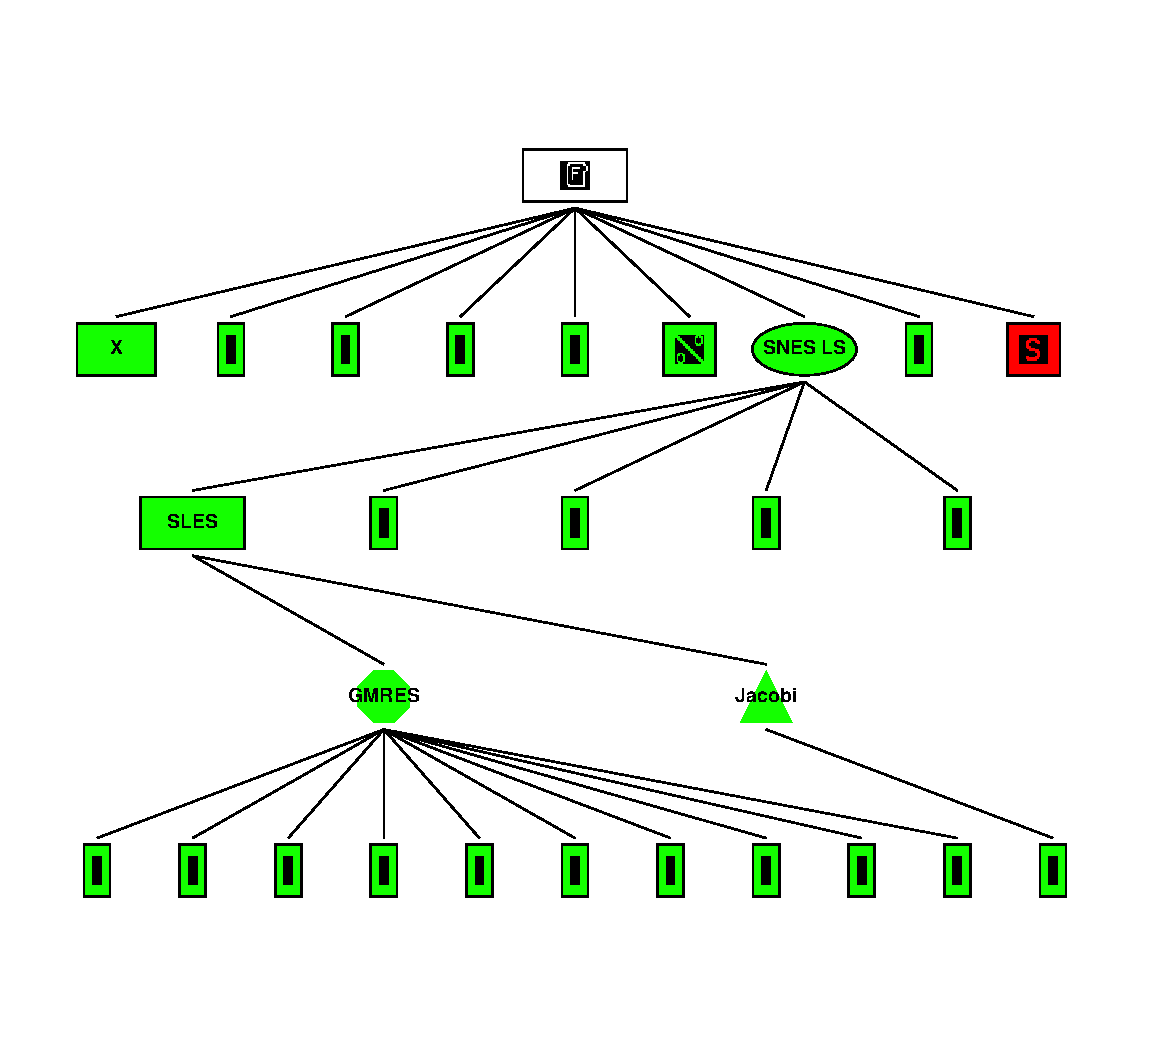
\psfig{file=treep.ps,height=5.0in,width=5.0in}
\caption{A Sample PETScView Object Tree}
\label{example_tree}
\end{figure}

\subsection{Running PETScView}

Due to fundamental limitations of Tcl/Tk, PETScView can only be run with 
relatively small log files (at most a couple thousand events). If the user
generates a very large log file, Tcl/Tk will hang and often swamp 
the machine. 

To begin PETScView, the user should type {\tt petscview} from the UNIX shell prompt.
To load a PETSc log file, one runs PETScView, giving the log 
file name as a command line argument:
\begin{verbatim}
   petscview Log.0
\end{verbatim}
This command invokes PETScView and automatically loads and
interprets the profiling data contained in the file {\tt Log.0}.
PETScView can also be run without a log file given as a command
line argument.  In this case, the user must load the log file from
within PETScView.  To do this, the user selects the ``Open File''
command from the file menu.  PETScView will automatically
present the user with another window from which the file can be
selected.

PETScView supports several additional command line arguments, as
listed in Table \ref{PETScView_command_line_options}.  Note that the
command line options override the default values within the user's
{\tt .petscviewrc} file, which is discussed further in
the following section. \findex{.petscviewrc}

\begin{table}
\begin{center}
\begin{tabular}{ll}
{\bf Argument}                  & {\bf Purpose} \\
\hline
{\tt -def\_file filename}       & The location of the definitions file \\
{\tt -time}                    & Show the time \\
{\tt -notime}                  & Do not show the time \\
{\tt -stepsize N}              & Set the stepsize to N \\
{\tt -delay N}                 & Set the delay to N milliseconds \\
{\tt -printer\_dest DESTINATION}& Set the destination (File or Printer) \\
{\tt -print\_command COMMAND}   & Set the postscript print command \\
{\tt -printer PRINTER}         & Specify the printer \\
{\tt -print\_orientation 1 or 0} $\:\:\:$ & 1 = landscape , 0 = portrait \\
{\tt -print\_color}             & Specify color mode (color, gray, mono) \\
\hline
\end{tabular}
\end{center}
\caption{PETScView Command Line Options}
\label{PETScView_command_line_options}
\end{table}

\subsection{Loading a Configuration File}

PETSc configuration files contain information that
determines the graphical representation of PETSc objects within PETScView.
Whenever PETScView is invoked, a configuration file
is automatically read.  The location of this file is specified in
{\tt .petscviewrc}, which is stored in the user's home directory.  By
default, {\tt .petscviewrc} points to the configuration file,
({\tt \$PETSC\_DIR/bin/petscview.cfg}); however, this can be
changed to point to a configuration file created by the application
programmer.  Section \ref{sec:petscview_advanced} gives
more information about changing the {\tt .petscviewrc} file.

Even though PETScView loads a definitions file whenever it is
initially run, a file of new definitions can be loaded from within
PETScView at any time.  This command is found in the file menu.
Loading a new definitions file will automatically update all PETSc
objects.

\subsection{Printing a PETScView Object Tree}

The ``print'' command of the file menu displays a dialog box from
which the user can change the printing options.  The default values
are loaded from {\tt .petscviewrc} when PETScView is first run.  When
the proper options are set for printing, one clicks on the ``print''
button or presses ``return''.  If the user is printing to a file,
another dialog box will appear from which the user may specify the
output filename.

{\em Note}:  Currently, PETScView  prints trees of size less
than 1024x768 (measured in pixels).  If the scrollbars are needed to
view any parts of a tree, it is very unlikely that the whole tree will
be printed.  This situation presents no problem, however, when the tree is
printed to a file.

\subsection{Exiting PETScView}

To exit PETScView, one selects the ``Exit'' option of the file
menu.  When this action is confirmed, PETScView will terminate
and return the user to the calling shell.

\subsection{The PETScView Simulation}

\subsubsection{Navigation}

Once a file has been loaded by PETScView, the user can navigate
through the simulation by using PETScView's play bar.  The play
bar is located at the bottom of the window and contains buttons whose
appearances and functioning resemble the buttons on a tape player.
From left to right, these buttons have the following functions:
\begin{itemize}
\item Rewind - Rewinds the simulation to the zeroth step.
\item Step Backward - Steps backward through the simulation.
\item Play Backward - Plays the simulation in reverse with an appropriate delay between steps.  
\item Stop - Brings the simulation to a halt.
\item Play Forward - Plays forward through the simulation with an appropriate delay between steps.
\item Step Forward - Steps forward through the simulation
\item Finish - Immediately jumps to the last step of the simulation.
\end{itemize}

In addition to the play bar buttons, the scale directly below these
buttons enables the user to navigate to an arbitrary position in the
simulation.  To use the scale, one clicks the left mouse button at
the desired position on the scale.  (The scale ranges from the zeroth
step to the last step of the simulation.)  The scale is scaled and
labeled appropriately.

All of the above functions can also be accessed through the ``player''
menu.  Selecting the player menu lists the commands in addition to
their accelerator keys.  The player menu also contains two additional
commands that allow the user to jump to an arbitrary step in the
simulation or to an arbitrary time during the simulation.  When one of
these commands is invoked, the user is prompted for the proper target
jump value.

\subsubsection{The View Menu}

The View menu contains several additional commands that can be useful
in the profiling of a PETSc program.  These commands enable the user
to view the raw profiling data as well as various statistics about
program performance.

\subsubsection{Changing Viewer Options}

The ``options'' menu allows the user to change certain options that
are set by default whenever PETScView is initially invoked.
(The default values are defined in {\tt .petscviewrc}.) These options
include the step size when stepping through the simulation, the delay
between events when playing through the simulation, and the colors
chosen to denote the internal states of the PETSc objects.

The simulation's step size can be changed at any time during the
simulation by selecting the ``Step size'' command of the ``Options''
menu.  Whenever the user clicks on the this selection, a dialog box
appears prompting the user for the desired step size.  Valid step
sizes range from $1$ to the total number of events in the simulation.

To change the delay, one selects the ``delay'' command of the options
menu.  A cascading menu presents the user with a few built-in delays,
which include none, real-time, and second delay.  (The real-time
delay option causes delays between events in the simulation to be
proportionate to the delays in the actual execution of the PETSc
program.)  To specify a user-defined delay, the user clicks on
the ``after delay'' selection.  Then the user will be
presented with a dialog box in which the user can specify the desired
delay in milliseconds.  Only values ranging from $1$ to $2000$ are
valid.

The final selection on the ``Options'' menu presents the user with a
cascading menu with entries that allow the user to change PETScView's
object color-coding scheme.  Selecting any one of the
entries presents the user with another window from which the color may
be chosen.  (The colors are taken from {\tt /usr/lib/X11/rgb.txt}.)

\subsection{Advanced Features}
\label{sec:petscview_advanced}

PETScView allows the user to define/redefine the graphical
representation of PETSc objects.  To do so, the user creates a
configuration file, a Tcl script file, which includes specific
definitions for group shapes, group labels, object icons, object
labels, and action strings.  Whenever PETScView is invoked, a
configuration file is read from the location specified in the {\tt
.petscviewrc} file.  By default, it is set to point to the
configuration file included with the PETSc package ({\tt
\$PETSC\_DIR/bin/petscview.cfg}).  Allowing the application programmer
to create a customized configuration file enables PETScView to
interpret the profiling data even when new PETSc objects have been
created.

\subsubsection{Group Definitions}

\begin{table}
\begin{center}
\begin{tabular}{||l||l||} \hline
{\bf Group}                              & {\bf Object\_cookie} \\
\hline
Viewers                            &  0 \\
Index Sets                         &  1 \\
Vectors                            &  2 \\
Vector Scattering                  &  3 \\
Matrices                           &  4 \\
Draw (simple graphics)             &  5 \\
Line Graphs                        &  6 \\
Krylov Subspace Solvers            &  7 \\
Preconditioners                    &  8 \\
Simplified Linear Equations Solvers     &  9 \\
Grids                              & 10 \\
Stencils                           & 11 \\
Simplified Nonlinear Solvers       & 12 \\
Distributed Arrays                 & 13 \\
Matrix Scattering                  & 14 \\
\hline
\end{tabular}
\end{center}
\caption{PETSc Object Group Definitions}
\label{PETSc_object_definitions}
\end{table}

Each PETSc object group is identified by its integer-valued object
cookie.  Table \ref{PETSc_object_definitions} lists the
currently available object groups and their associated object cookies.
For each group of objects, the PETScView requires the following
definitions:
\begin{verbatim}
   set GroupShape(OBJECT_COOKIE) SHAPE 
   set GroupDesc(OBJECT_COOKIE) "GROUP DESCRIPTION"
\end{verbatim}
where {\tt OBJECT\_COOKIE} is the integer used to identify the group
of objects and {\tt SHAPE} is one of the predefined shapes used by
PETScView.  These shapes include
\begin{verbatim}
   Square                Wide_Rectangle       Down_Triangle
   Thin_RectangleV       Tall_Oval            Octagon
   Thin_RectangleH       Wide_Oval            Circle
   Rectangle             Up_Triangle
\end{verbatim}

{\tt GROUP DESCRIPTION} is a line of text enclosed by quotes to describe the object group.  For example, vectors have the following group descriptions:
\begin{verbatim}
   set GroupShape(2) Thin_RectangeV 
   set GroupDesc(2)  Vectors
\end{verbatim}

\subsubsection{Object Definitions}

Within each group, the object is identified with the use of a second integer ({\tt OBJECT\_TYPE}).  This specifies the type of object within the object group.  PETScView requires both a name and an icon to be defined for every object.  These definitions have the following syntax:
\begin{verbatim}
   set Icon(OBJECT_COOKIE,OBJECT_TYPE) "-text TEXT" or 
   set Icon(OBJECT_COOKIE,OBJECT_TYPE) "-bitmap @BITMAP_LOC"
   set Name(OBJECT_COOKIE,OBJECT_TYPE) "OBJECT DESCRIPTION"
\end{verbatim}
where {\tt TEXT} is a short description of the object (used if a bitmap is inappropriate) and {\tt BITMAP\_LOC} is the location of the bitmap graphic.  The {\tt OBJECT DESCRIPTION} is a line of text used to describe the object.  As an example, we give the following definitions:
\begin{verbatim}
   set Icon(2,0) "-bitmap @$env(PETSC_DIR)/bitmaps/vector.bit" 
   set Name(2,0) "Sequential Vector" 
   set Icon(2,1) "-bitmap @$env(PETSC_DIR)/bitmaps/vectorp.bit" 
   set Name(2,1) "Parallel Vector"
\end{verbatim}
Notice the syntax that Tcl requires for the location of the bitmap.
The bitmap location must be preceded by a $@$ in order for PETScView
the work properly.  {\tt \$env(\$PETSC\_DIR)} is used to access the
value of the environmental variable {\tt PETSC\_DIR}.  To use the
value of any other environmental variables in specifying a file
location, one must use in the expression the following syntax:
\begin{verbatim}
   $env(ENVIRONMENTAL_VARIABLE)
\end{verbatim}

To create one's own bitmap picture to represent an
object, the user creates the bitmap using a program such as {\tt bitmap.}
Once this is done, PETScView must know the location of the
bitmap.  The user must specify the precise location in
the file system where the bitmap graphic can be found.  For example,
suppose that one creates a new bitmap to symbolize a parallel vector.
Since the bitmap is located in the user's home directory, the
following definition will {\em not} create an error:
\begin{verbatim}
   set Icon(2,1) "-bitmap $env(HOME)/vectorp.bit"
\end{verbatim}

More examples on defining additional PETSc objects and informat
about how PETSc defines the object types, are given in 
{\tt \$PETSC\_DIR/bin/petscview.cfg}.

\subsubsection{Action Strings}

When certain actions occur during the execution of a PETSc program,
these actions are also recorded in the profiling data.  Once again,
PETSc uses an integer to specify the type of action that is being
performed.  PETScView interprets the actions using the
definitions contained in {\tt action()} string definitions.  These
definitions are also located in the configuration file.  An action
definition has the following syntax:
\begin{verbatim}
   set Action(ACTION_ID) "ACTION"
\end{verbatim}
where {\tt ACTION\_ID} is an integer that encodes the action and {\tt
ACTION} is a descriptive string.  Currently, PETScView uses the action
definitions as defined in {\tt petscview.cfg}.

\section{Using PETScOpts}
\label{sec:petscopts}

PETScOpts is a PETSc utility program that enables the application
programmer to modify his or her personal {\tt .petscrc} file.  As
described in Section \ref{sec:options}, the {\tt .petscrc} file
contains a list of options that will be passed to a PETSc program
whenever it is executed.  This file has the following format:
\begin{verbatim}
   -optionname possible_value
   -anotheroptionname possible_value
\end{verbatim}
Even though this file can be manually modified by the application
programmer with any text editor, PETScOpts greatly simplifies this
task.

\subsection{Running PETScOpts}

The command {\tt petscopts} will invoke PETScOpts from the UNIX
shell prompt.  Any entries contained in the {\tt .petscrc} file of the
user's home directory will automatically be interpreted by PETScOpts.
Once inside PETScOpts, a number of entry boxes, check
buttons, radio buttons, and other widgets allow the application
programmer to specify the options that should be saved in the {\tt
.petscrc} file for future use.

PETScOpts can also write the PETSc command line options to a file
other than the default {\tt .petscrc} file. To do so, run PETScOpts
with the file name as a command line argument:
\begin{verbatim}
   petscopts file_name
\end{verbatim}
From within PETScOpts, a different file can be loaded at any time
by selecting the ``Open file'' option of the file menu.

\subsection{Getting Help}

Even though many of PETSc's command line options are self-explanatory,
a single descriptive line of text is displayed at the bottom of the
window whenever the pointer is positioned over any check button, radio
button, or entry that specifies an option.

\subsection{Exiting PETScOpts}

The user can exit PETScOpts at any time by selecting the exit
button from the file menu.  If a {\tt .petscrc} file was loaded when
PETScOpts was initiated, the user is asked whether the current or
original settings (or neither) should be saved in {\tt .petscrc}.

%------------------------------------------------------------------

\chapter{Design and Implementations of the  Abstract Classes}
\label{chapter:design}

PETSc 2.0 is designed using strong data encapsulation.  Hence,
any collection of data (for instance, a sparse matrix) is stored in 
a way that is completely private from the application code. The application 
code can manipulate the data only through a well-defined interface, as it 
does {\em not} know how the data is stored internally. 

PETSc is designed around several components (e.g. {\tt Vec} (vectors),
{\tt Mat} (matrices, both dense and sparse)). Each component has
\begin{itemize}
\item Its own include file {\tt \$(PETSC\_DIR)/include/<component>.h} 
\item Its own directory, {\tt \$(PETSC\_DIR)/src/<component>}
\item An abstract data structure defined in  the file
      {\tt \$(PETSC\_DIR)/src/<component>/<component>impl.h}.
      This data structure is shared by all the different implementations of the 
      component. For example, for matrices it is shared by dense,
      sparse, parallel, and sequential formats.
\item An abstract interface that defines the application callable 
      functions for the component. These are defined in the directory
      {\tt \$(PETSC\_DIR)/src/<component>/interface}.
\item One or more actual implementations of the components (for example,
      sparse uniprocessor and parallel matrices implemented with the AIJ storage format).
      These are each in a subdirectory of 
      \break {\tt \$(PETSC\_DIR)/src/<component>/impls}. Except in rare circumstances data 
      structures defined here should not be referenced from outside this 
      directory.
\end{itemize}

Each type of object, for instance a vector, is defined in its own
include file, by {\tt typedef \_p\_Object* Object;}, (for example, 
{\tt typedef \_p\_Vec* Vec;}).  This organization
allows the compiler to perform type checking while at the same time
completely removing the details of the implementation of {\tt
\_p\_Object} from the application code. The exact details of {\tt
\_p\_Object} may be changed at link time. This capability is extremely important
because it allows the library internals to be changed
without altering or recompiling the application code.

Polymorphism is supported through the directory {\tt \$(PETSC\_DIR)/src/<component>/interface},
which contains the code that implements the abstract interface to the
operations on the object.  Essentially, these routines do some error
checking of arguments and logging of profiling information 
and then call the function appropriate for the
particular implementation of the object. The name of the abstract
function is {\tt ObjectOperation}, for instance, {\tt MatMult} or {\tt PCCreate}, while
the name of a particular implementation is 
\break{\tt ObjectOperation\_Implementation}, for instance, 
{\tt MatMult\_SeqAIJ} or {\tt PCCreate\_ILU}. These naming
conventions are used to simplify code maintenance.

Each object structure (named {\tt \_p\_Object}) consists of three parts:
a common PETSc header (defined in {\tt include/phead.h},
a pointer to a list of operations for the
object, and any additional information that is appropriate for the
particular abstract object.  The PETSc header includes an integer
cookie, an integer type, an MPI communicator, a function pointer that
indicates a destroy routine, and a function pointer that indicates a
viewer routine. The header can also contain additional records.
Several routines are provided for manipulating data within the header,
including
\begin{verbatim}
   int PetscObjectGetComm(PetscObject object,MPI_Comm *comm) 
\end{verbatim}
which returns in {\tt comm} \findex{PetscObjectGetComm()}
\sindex{communicator} the MPI communicator associated with the
specified object.

After the header, each PETSc object contains a pointer to a list of
operations for the object.  For example, the vector operations include
norms, assembly routines, scatters, gathers, etc.  Finally,
information that is appropriate for the particular abstract object is
included. Generally, this information includes a pointer to data used
by a particular implementation.  For example, the {\tt \_p\_Vec}
structure is given by
\begin{verbatim}
   struct _p_Vec {
      PETSCHEADER
      struct _VeOps ops;
      void          *data;
   };
\end{verbatim}

\section{Names}
Consistency of names for variables, functions, etc. is extremely 
important in making the package both usable and maintainable.
We use several conventions:
\begin{itemize}
\item All function names and enum types consist of words, each of 
      which is capitalized, for example {\tt SLESSolve()} and 
      {\tt MatGetReordering()}.
\item All enum elements and macro variables are capitalized. When
      they consist of several
      complete words, there is an underscore between each word.
\item Functions that are private to PETSc (not callable by the 
      application code) either
      \begin{itemize}
        \item have an appended {\tt \_Private} (for example, 
           {\tt StashValues\_Private}) or
        \item have an appended {\tt \_ObjectSubtype} (for example,
           {\tt MatMult\_SeqAIJ}).
      \end{itemize}

      In addition, functions that are not intended for use outside
      of a particular file are declared static.
\item Function names in structures are the same as the base application
      function name without the object prefix, and all are in small letters. 
      For example, {\tt MatMultTrans()} has a structure name of 
      {\tt multtrans()}.
\item Each application usable function begins with the name of the object, 
      for example, {\tt ISInvertPermutation} or {\tt MatMult}. 
\end{itemize}

\section{Coding Conventions and Style Guide}

Within the PETSc source code, we adhere to the following guidelines
so that the code is uniform and easily maintainable:

\begin{itemize}
\item All PETSc function bodies are indented two characters.
\item Each additional level of loops, if statements, etc. is indented
      two more characters.
\item Wrapping lines should be avoided whenever possible.
\item Source code lines should not be more than 120 characters wide.
\item The macros {\tt SETERRQ()} and {\tt CHKERRQ()} should be on the 
      same line as the routine to be checked unless this violates the 
      120 character width rule. Try to make error messages short, but 
      informative.
\item The local variable declarations should be aligned. For example,
      use the style
\begin{verbatim}
   int    i,j;
   Scalar a;
\end{verbatim}
instead of
\begin{verbatim}
   int i,j;
   Scalar a;
\end{verbatim}
\item All local variables of a particular type (e.g., {\tt int}) should be 
      listed on the same line if possible; otherwise, they should be listed
      on adjacent lines.
\item Equal signs should be aligned in regions where possible.
\item For routines of more than a few lines, there should be a blank line
      between the local variable declarations and the body of the function.
\item Indentation for {\tt if} statements should be done either as
\begin{verbatim}
   if (  ) {
     ....
   }
   else {
     ....
   }
\end{verbatim}
or as
\begin{verbatim}
   if (  ) {
     ....
   } else {
     ....
   }
\end{verbatim}
\item {\em No} tabs are allowed in {\em any} of the source code.
\end{itemize}

\section{Option Names}

Since consistency simplifies usage and code maintenance, the names of
PETSc routines, flags, options, etc. have been selected with great care.
The default option names are of the form {\tt -package\_subpackage\_name}.  
For example, the option name for the basic convergence tolerance for 
the KSP package is {\tt -ksp\_atol}. In addition, operations in different 
packages of a similar nature have a similar name.  For example, the option
name for the basic convergence tolerance for the SNES package is 
{\tt -snes\_atol}.

%- - - - - - - - - - - - - - - - - - - - - - - - - - - - - - - - - - -
\section{Implementation of Profiling}
\label{sec:profimpl}

This section provides details about the implementation of event
logging and profiling within PETSc.   Chapter~\ref{ch:profiling}
gives information about using the profiling in application codes. 

The interface for profiling in PETSc is contained in the file 
{\tt \$(PETSC\_DIR)/include/petsclog.h}. It includes \findex{PLogObjectCreate()}
\begin{verbatim}
   PLogObjectCreate(PetscObject h);
\end{verbatim}
which logs the creation of any PETSc object. This should be included in 
any PETSc source code that uses {\tt PetscHeaderCreate()}. 

Just before an object is destroyed, it is logged
with \findex{PLogObjectDestroy()} 
\begin{verbatim}
   PLogObjectDestroy(PetscObject h);
\end{verbatim}

If an object has a clearly defined parent object (for instance, when 
a work vector is generated for use in a Krylov solver), this information
is logged with the command, \findex{PLogObjectParent()}
\begin{verbatim}
   PLogObjectParent(PetscObject parent,PetscObject child);
\end{verbatim}
It is also useful to log information about the state of an object, as can
be done with the command \findex{PLogObjectState()}
\begin{verbatim}
   #if defined(PETSC_LOG)
   PLogObjectState(PetscObject h,char *format,...);
   #endif
\end{verbatim}
For example, for sparse matrices we usually log the matrix 
dimensions and number of nonzeros.

As discussed in the preceding section, events are logged using the 
pair \findex{PLogEventBegin()}
\begin{verbatim}
   PLogEventBegin(int event,PetscObject o1,PetscObject o2,PetscObject o3,PetscObject o4);
   PLogEventEnd(int event,PetscObject o1,PetscObject o2,PetscObject o3,PetscObject o4);
\end{verbatim}
This logging is usually done in the abstract
interface file for the operations, for example, {\tt src/mat/src/matrix.c}.

Several routines that will be used rarely by the 
application programmer \findex{PLogPrintSummary()}
are \findex{PLogBegin()} \findex{PLogDump()} \findex{PLogAllBegin()} 
\begin{verbatim}
   PLogBegin();
   PLogAllBegin();
   PLogDump(char *filename);
   PLogPrintSummary(FILE *fd);
\end{verbatim}
These routines are normally called by the {\tt PetscInitialize()}
and {\tt PetscFinalize()} routines when the option {\tt -log}, 
{\tt -log\_summary}, or 
{\tt -log\_all} is given.

\section{The Various Matrix Classes}
\label{sec:matclasses}

PETSc provides a variety of matrix implementations, since no single
matrix format is appropriate for all problems. The following sections
briefly describe the ever-expanding assortment of matrix types within PETSc.

\subsection{Sequential AIJ Sparse Matrices}

The default matrix representation within PETSc is the general sparse
AIJ format (also called the Yale sparse matrix format or compressed
sparse row format, CSR). Section~\ref{sec:matsparse} describes this
matrix type.

\subsection{Parallel AIJ Sparse Matrices}

%
%  Temp remove
%
%The implementation of the parallel AIJ matrix data structure is 
%described in detail within \cite{petsc-mpi-paper}.

\subsection{Sequential Block AIJ Sparse Matrices}

The sequential and parallel block AIJ formats, which are extensions of
the AIJ formats described above, are intended especially for use with
multicomponent PDEs.  The block variants store matrix elements by
fixed-sized dense {\tt nb} $\times$ {\tt nb} blocks, where currently
{\tt nb} ranges from two through five.  These formats are fully
compatible with standard Fortran77 storage.  That is, the stored row
and column indices can begin at either one (as in Fortran) or zero.

The routine for creating a sequential block AIJ matrix with {\tt m} 
rows, {\tt n} columns, and a block size of {\tt nb} is
\begin{verbatim}
   ierr = MatCreateSeqBAIJ(MPI_Comm comm,int nb,int m,int n,int nz,int *nnz, Mat *A)
\end{verbatim}
\findex{MatCreateSeqBAIJ} 
The arguments {\tt nz} and {\tt nnz} can be used to preallocate matrix
memory by indicating the number of {\em block} nonzeros per row.  For good
performance during matrix assembly, preallocation is crucial; however, the
user can set {\tt nz=0} and {\tt nzz=PETSC\_NULL} for PETSc to dynamically
allocate matrix memory as needed.  Section~\ref{sec:matsparse}
discusses preallocation for the AIJ format; extension to the block AIJ
format is straightforward.

Note that the routine {\tt MatSetValuesBlocked()}
\findex{MatSetValuesBlocked()} can be used for more efficient matrix assembly
when using the block AIJ format.

\subsection{Parallel Block AIJ Sparse Matrices}

Parallel block AIJ matrices with block size {\t nb} can be created with
the command \findex{MatCreateMPIBAIJ()}
\begin{verbatim}
   ierr = MatCreateMPIBAIJ(MPI_Comm comm,int nb,int m,int n,int M,int N,int d_nz,
                          int *d_nnz, int o_nz,int *o_nnz,Mat *A);
\end{verbatim}
{\tt A} is the newly created matrix, while the arguments {\tt m}, {\tt n}, 
{\tt M}, and {\tt N}, indicate the number of local rows and columns and
the number of global rows and columns, respectively. Either the local or
global parameters can be replaced with {\tt PETSC\_DECIDE}, so that 
PETSc will determine \findex{PETSC_DECIDE} them.
The matrix is stored with a fixed number of rows on 
each processor, given by {\tt m}, or determined by PETSc if {\tt m} is
{\tt PETSC\_DECIDE}.

If one does not use {\tt PETSC\_DECIDE} for
{\tt m} and {\tt n} then he must ensure that they are chosen to be
compatible with the vectors. To do this, one first considers the product 
$y = A x$. The {\tt m} that one uses in {\tt MatCreateMPIBAIJ()}
must match the local size used in the {\tt VecCreateMPI()} for {\tt y}.
The {\tt n} used must match that used as the local size in 
{\tt VecCreateMPI()} for {\tt x}. 

The user must set {\tt d\_nz=0}, {\tt o\_nz=0}, {\tt d\_nnz=PETSC\_NULL}, and 
{\tt o\_nnz=PETSC\_NULL} for PETSc to control dynamic allocation of matrix
memory space.  Analogous to {\tt nz} and {\tt nnz} for the routine 
{\tt MatCreateSeqBAIJ()}, these arguments optionally specify 
block nonzero information for the diagonal ({\tt d\_nz} and {\tt d\_nnz}) and 
off-diagonal ({\tt o\_nz} and {\tt o\_nnz}) parts of the matrix. 
For a square global matrix, we define each processor's diagonal portion 
to be its local rows and the corresponding columns (a square submatrix);  
each processor's off-diagonal portion encompasses the remainder of the
local matrix (a rectangular submatrix).  
Section~\ref{sec:matsparse} gives an example of preallocation for
the parallel AIJ matrix format; extension to the block parallel AIJ case
is straightforward.

\subsection{Sequential Dense Matrices}

PETSc provides both sequential and parallel dense matrix formats,
where each processor stores its entries in a column-major array in the
usual Fortran77 style.  Section~\ref{sec:matdense} provides details
on creating these matrices.

\subsection{Parallel Dense Matrices}

The parallel dense matrices are partitioned by rows across the
processors, so that each local rectangular submatrix is stored in the
dense format described above.

\subsection{Parallel Cyclic Block Dense Matrices}
Not yet implemented.

\subsection{Parallel BlockSolve Sparse Matrices}

PETSc provides a parallel, sparse, row-based matrix format that is
intended for use in conjunction with the ILU and ICC preconditioners
in BlockSolve95.  Section~\ref{sec:ilu_icc} gives details on this
matrix type.

\subsection{Block Diagonal Sparse Matrices}
\label{sec:bdiag}

Storage \sindex{block diagonal matrix storage} by block diagonals is
available in both uniprocessor and parallel versions, although currently
only a subset of matrix operations is supported.  Each element of
a block diagonal is defined to be a square dense block of size {\tt
nb} $\times$ {\tt nb}, where conventional diagonal storage results for
{\tt nb}=1.  Such storage is particularly useful for multicomponent PDEs
discretized on regular grids.

The routine for creating a uniprocessor block diagonal matrix with {\tt m} 
rows, {\tt n} columns, and a block size of {\tt nb} is
\begin{verbatim}
   ierr = MatCreateSeqBDiag(PETSC_COMM_SELF,int m,int n,int nd,int nb,int *diag,
                                   Scalar **diagv,Mat *A);
\end{verbatim}
The \findex{MatCreateSeqBDiag} argument {\tt nd} is the number of 
block diagonals, and {\tt diag} is
an array of block diagonal numbers.  For the matrix element $A_{ij}$,
where $i$ and $j$ respectively denote the row and column number of the 
element, the block diagonal number is computed using integer division by
\[ {\tt diag} = i/nb - j/nb. \]
If matrix storage space is allocated by the user, the argument {\tt diagv} 
is a pointer to the actual diagonals (in the same order as the {\tt diag} 
array).  For PETSc to control memory allocation, the user should merely
set {\tt diagv=PETSC\_NULL}.

A simple example of this storage format is illustrated below for block
size {\tt nb}=1. 
Here {\tt nd} = 4 and {\tt diag} = [2, 1, 0, -3]. The
diagonals need not be listed in any particular order, so that
{\tt diag} = [-3, 0, 1, 2] or {\tt diag} = [0, 2, -3, 1] would also
be valid values for the {\tt diag} array. 

\begin{center}
\begin{tabular}{| c c c c c c |}
\hline
a00  &0    &0    &a03  &0    &0\\
a10  &a11  &0    &0    &a14  &0\\
a20  &a21  &a22  &0    &0    &a25\\
0    &a31  &a32  &a33  &0    &0\\
0    &0    &a42  &a43  &a44  &0\\
0    &0    &0    &a53  &a54  &a55\\
\hline
\end{tabular}
\end{center}

\subsection{Parallel Block Diagonal Sparse Matrices}

The parallel block diagonal matrices are partitioned by rows across
the processors, so that each local rectangular submatrix is stored by
block diagonals as described above.  The routine for creating a
parallel block diagonal matrix with {\tt m} local rows, {\tt M} global
rows, {\tt n} global columns, and a block size of {\tt nb} is
\begin{verbatim}
   ierr = MatCreateMPIBDiag(PETSC_COMM_SELF,int m,int M,int N,int nd,int nb,int *diag,
                            Scalar **diagv,Mat *A);
\end{verbatim}
Either the {\tt m} or {\tt M} can be set to {\tt PETSC\_DECIDE} for PETSc
to determine the corresponding quantity.

\section{Other Libraries and Packages}

It is not the intention of PETSc to provide all of the software pieces 
to solve a user's application problem. The intention is that other 
libraries can provide the pieces that are not in PETSc.  Unfortunately, 
not many robust, general-purpose, easy-to-use software packages 
are available, and some of those that do exist have a very low-level 
user interface. 

\sindex{petsc-maint}  \sindex{SPARSPAK}
To simplify the use of certain packages, we have integrated
into PETSc an interface to those packages. At the moment, these include
parts of LAPACK, BLAS, BlockSolve95, and the reordering routines in 
SPARSPAK.  We invite users to let us know (by writing to petsc-maint@mcs.anl.gov)
whether they need particular libraries that 
are related to PETSc for an application; we may try to provide 
easy-to-use PETSc interfaces for them.

To allow the portable use of BLAS and LAPACK from C, we constructed a
new include file, 
\break{\tt \$(PETSC\_DIR)/include/pinclude/plapack.h}, that uses defines to make
a uniform naming scheme for BLAS (all routines begin with BL) and
LAPACK (all routines begin with LA). This file incorporates function
prototypes for the BLAS and LAPACK routines used. In addition, the
include file deals with different Fortran77 compilers' treatment of
function names (for instance, Sun compilers put an underscore at the
end of all functions created in Fortran77).  The include file also
deals with the fact that on Crays, C double precision is the same as
Fortran77 single precision.  Lastly, it also calls the appropriate
complex LAPACK and BLAS routines when needed.

